%\documentclass[a4paper,11pt]{article}
\documentclass[a4paper,11pt]{scrartcl}

\usepackage[utf8]{inputenc}
\usepackage[italian]{babel}

\usepackage{graphicx} %for includng images
\graphicspath{{img/}}

\usepackage{siunitx} % package for deciBel and other units
\usepackage{amsmath} % package for ``cases'' and other matemagical stuff
\usepackage[american]{circuitikz} % circuit drawer
\ctikzset{/tikz/circuitikz/bipoles/length=1cm} %dimensione componenti
\usepackage{subcaption}  %per immagini multiple
%\usepackage{xcolor} % Colori!
\usepackage{colortbl} %colori nelle tabelle!!
\usepackage{multirow} %righe doppie nelle tabelle
\usepackage{makecell} %multirow box
\usepackage{hyperref}
\usepackage{cancel} %utile a cancellare termini nelle equazioni
\hypersetup{ % vedi https://it.overleaf.com/learn/latex/hyperlinks
    colorlinks=true,
    linkcolor=blue,
    filecolor=magenta,      
    urlcolor=blue
}
\usepackage{esint} %utile a plottare integrali doppi chiusi
\usepackage{tikz-3dplot} %per fare plot in 3 assi
\tdplotsetmaincoords{70}{110} %rotazione globale per tutte le rappresentazioni 3D

\usepackage{pgfplots} % plot 2D
\pgfplotsset{compat=1.17}

\usepackage{amssymb} % simboli come R^3

\usepackage{float} %gestire le posizioni dei 'float' es tabella lez 16

\usepackage{listings} %inserire codice MATLAB colorato
\usepackage{xcolor}
\usepackage[framed]{matlab-prettifier}

\title{Appunti di Principi di Ingegneria Elettrica II}
\author{Daniele Olivieri}
\date{\today}

\pdfinfo{%
  /Title    ()
  /Author   ()
  /Creator  ()
  /Producer ()
  /Subject  ()
  /Keywords ()
}
%\includeonly{22_dai_campi_ai_modelli,23_conduzione_FEM_resistenza}
\begin{document}
\maketitle
Ti piacciono i miei appunti? Saranno sempre liberi e gratuiti ma puoi sostenermi con una donazione cliccando \href{https://www.paypal.com/donate?hosted_button_id=7KELP768NJSYW}{QUI}

Puoi accedere ai codici sorgente seguendo questo \href{https://github.com/FlashNoob98/appunti_principi_II_unina}{link} invece.
\setcounter{tocdepth}{2}
\tableofcontents
\setlength\arrayrulewidth{1.2pt} %larghezza righe tabelle
\section{Introduzione ai circuiti dinamici}
Tutti i circuiti che contengono componenti come
resistori, induttori e condensatori, generatori indipendenti di tensione e corrente ai quali si associa 
una tensione impressa o una corrente impressa vengono detti circuiti lineari tempo invarianti (LTI).

Se vi sono anche bipoli tempo-varianti come interruttori che si chiudono o si aprono, il circuito
si definisce lineare tempo variante (LTV).

Preso un generico circuito, si vuole determinare una tensione o un'intensità di corrente di un generico
bipolo.

\textbf{Strumenti a disposizione:}

\begin{itemize}
\item Equazioni di interconnessione:
\begin{equation} \label{eq:leggi_kirchooff}
\begin{cases}
        \text{LKC} & \forall \text{ nodo } \sum_{k} (\pm) i_k(t) = 0\ \forall\ t \\
        \text{LKT} & \forall \text{ maglia } \sum_{h} (\pm) v_n(t) = 0\ \forall\ t
\end{cases}
\end{equation}

\item Relazioni caratteristiche dei bipoli coerenti con la scelta dei versi delle grandezze (convenzione del generatore o dell'utilizzatore).
\begin{equation}
\begin{cases}
v_R  = R\cdot i \\
v_L  = L\frac{di_L}{dt} \\
i_C  = C\frac{dv_C}{dt} \\
v_e  = e(t)\\
i_j  = j(t) \\
\end{cases}
\end{equation}
\begin{equation*}
\begin{cases}
\text{interruttori in chiusura a t=0: }  {t<0,\ i = 0\ \forall\ v;\ t > 0,\ v = 0\ \forall\ i} \\
\text{interruttori in apertura a t=0: }  {t<0,\ v = 0\ \forall\ i;\ t > 0,\ i = 0\ \forall\ v} 
\end{cases}
\end{equation*}
\end{itemize}

Le equazioni di interconnessione non sono tutte indipendenti ma è sempre possibile
costruire un set di equazioni indipendenti scegliendo \textit{n-1} nodi o \textit{n-l-1} maglie fondamentali,
dove n ed l sono rispettivamente il numero di nodi e lati del grafo connesso.

NOTA: per ogni induttore la potenza assorbita:
$$ P^a(t) = v_l\cdot i_l = L \frac{di_L}{dt}\cdot i_l = \frac{d}{dt} \left[\frac{1}{2}Li_L^2\right] = \frac{dW_m}{dt} $$ 
L' energia immagazzinata nel campo magnetico dell'induttore invece:
$$\Delta W^a(t_1,t_2) = \int_{t_1}^{t_2} P^a(\tau)d\tau = W_m (t_2) - W_m(t_1) $$
Se in un certo istante di tempo l'induttore presenta una certa quantità di energia in Joule [\si{\joule}] quella sarà la massima energia estraibile.

Per ogni condensatore invece potenza ed energia sono così definite:
$$P^a(t) = \frac{d}{dt} W_e;\ W_e(t) = \frac{1}{2} CV_c^2$$
L'energia sarà immagazzinata mediante il campo elettrico.

Si ha quindi un sistema di equazioni circuitali in cui si ha una parte algebrica con le caratteristiche adinamiche, ossia con caratteristiche
non differenziali e non integrali, più una parte differenziale data dai bipoli dinamici come condensatori e induttori.
In letteratura un sistema simile si indica con DAE (Differential Algebric Equation), differente
dalla ODE (Ordinary Differential Equation).

Le tecniche utilizzate in teoria dei circuiti mirano a trasformare una DAE in una ODE, ossia 
formulare le equazioni circuitali come equazioni differenziali ordinarie, per operare questa trasformazione si fa 
riferimento alla dinamica delle sole {variabili di stato}: $i_l(t),\ v_c(t)$

La loro conoscenza permette di esprimere tutte le altre variabili attraverso relazioni algebriche, vengono definite
variabili \textit{slaved}, perché subordinate alle prime.

Per eseguire ciò si richiama una procedura generale per l'analisi di circuiti lineari tempo varianti (LTV).
Questa procedura si basa su un'analisi a intervallo: si partiziona l'asse dei tempi in intervalli in ciascuno dei 
quali esiste un circuito tempo invariante (LTI) equivalente a quello di partenza.

\begin{figure}[H] %tre stati diversi dello stesso circuito
\centering
 \begin{subfigure}{.3\textwidth}
  \centering
  \caption{configurazione generica}
  \begin{circuitikz}
   \draw (0,0) to [R] (1,0);
   \draw (0,0.6) to [L] (1,0.6);
   \draw (0,1.2) to [C] (1,1.2);
   \draw (0,1.8) to [V] (1,1.8);
   \draw (0,2.4) to [I] (1,2.4);
   \draw (0,3) to [closing switch] (1,3);
   \draw (0,3.6) to [opening switch] (1,3.6);
   \draw (-0.3,-0.3) rectangle (1.3,3.9);
  \end{circuitikz}
 \end{subfigure}
 \begin{subfigure}{.3\textwidth}
  \centering
  \caption{$t<0$}
  \begin{circuitikz}
   \draw (0,0) to [R] (1,0);
   \draw (0,0.6) to [L] (1,0.6);
   \draw (0,1.2) to [C] (1,1.2);
   \draw (0,1.8) to [V] (1,1.8);
   \draw (0,2.4) to [I] (1,2.4);
   \draw (0,3) to [open,o-o] (1,3);
   \draw (0,3.6) to [short] (1,3.6);
   \draw (-0.3,-0.3) rectangle (1.3,3.9);
  \end{circuitikz}
 \end{subfigure}
 \begin{subfigure}{.3\textwidth}
  \centering
  \caption{$t>0$}
  \begin{circuitikz}
   \draw (0,0) to [R] (1,0);
   \draw (0,0.6) to [L] (1,0.6);
   \draw (0,1.2) to [C] (1,1.2);
   \draw (0,1.8) to [V] (1,1.8);
   \draw (0,2.4) to [I] (1,2.4);
   \draw (0,3) to [short] (1,3);
   \draw (0,3.6) to [open,o-o] (1,3.6);
   \draw (-0.3,-0.3) rectangle (1.3,3.9);   
  \end{circuitikz}
 \end{subfigure}
\end{figure}

Supponendo che i generatori indipendenti abbiano grandezze \textbf{limitate}, ossia le tensioni impresse $e(t)$ e le correnti impresse $j(t)$,
in questa ipotesi si sa che le variabili di stato sono funzioni \textbf{continue} ossia:
\begin{equation*}
\begin{split}
i_L (0^+) & = i_L(0^-) \\
v_C (0^+) & = v_C(0^-)
\end{split}
\end{equation*}

La soluzione si determina trovando la dinamica delle variabili di stato in ciascun circuito ausiliario, "incollando" le soluzioni utilizzando la proprietà di continuità delle variabili di stato.

Il problema di risolvere circuiti lineari tempo varianti si scompone nel risolvere tanti circuiti lineari tempo invarianti. Una categoria semplice di circuiti tempo invarianti sono i
circuiti lineari del primo ordine (circuiti RC o RL) con un solo elemento dinamico.
\begin{figure}[H] %circuiti RC ed RL equivalenti
\centering
 \begin{subfigure}{.3\textwidth}
  \centering
  \begin{circuitikz}
   \draw (0,0) rectangle (1.6,1.7);
   \draw (0.3,0.3) to [I] (1.3,0.3);
   \draw (0.3,0.9) to [V] (1.3,0.9);
   \draw (0.3,1.5) to [R] (1.3,1.5);
   \draw (1.6,1.5) to [short,i=$i_C$] (2,1.5)
   to [C,v^=$v_C $] (2,0.4) to [short] (1.6,0.4);
  \end{circuitikz}
  \caption{Circuito RC}
 \end{subfigure} 
  \begin{subfigure}{.3\textwidth}
  \centering
  \begin{circuitikz}
   \draw (0,0) rectangle (1.6,1.7);
   \draw (0.3,0.3) to [I] (1.3,0.3);
   \draw (0.3,0.9) to [V] (1.3,0.9);
   \draw (0.3,1.5) to [R] (1.3,1.5);
   \draw (1.6,1.5) to [short,i=$i_L $] (2,1.5)
   to [L,v^=$v_L $] (2,0.4) to [short] (1.6,0.4);
  \end{circuitikz}
  \caption{circuito RL}
 \end{subfigure}
\end{figure}

Un bipolo adinamico lineare e un bipolo dinamico fanno subito pensare all'utilizzo dei teoremi di Thévenin e Norton, permettendo la riduzione del circuito 
adinamico ad un semplice generatore con un resistore equivalente.

Applicando ad esempio la LKT $e_0(t) = R_{th}\cdot C \frac{dV_C}{dt} + V_C$ si ha l'equazione di stato
del circuito e supponendo di conoscere $V_C(t=0) = V_0 $ allora la soluzione dell'equazione è:
$$V_C(t) = [V_0-V_{C_p}(0)] e^{-\frac{t}{\tau}} + V_{C_p}(t)$$ dove $\tau = R_{th}\cdot C$ e $V_{C_p}(t)$
è la soluzione a regime. 
 
Dopo un intervallo pari a $4\sim 5\ \tau$ si assume il processo di carica o scarica terminato.

Per il circuito RL 
$$I_L(t) = [I_0-I_{L_p}(0)]e^{-\frac{t}{\tau}} + I_{L_p}(t)$$ 
con $\tau = \frac{L}{R_{th}},\ I_0 = I_L (t=0)$

Osservazione: la soluzione generale del circuito RC, ossia la dinamica di $V_c(t)$ può essere espressa 
come la somma di due termini $V_{C_{tr}}(t)$ e $V_{C_p}(t)$, il primo transitorio, che tende a svanire se 
si attende un tempo sufficiente lungo, porta con se la \textit{memoria} dello stato iniziale, memoria che 
viene
persa quando $t>4\sim5\ \tau$, ammesso che $\tau$ sia positiva; esistono infatti alcune combinazioni di 
elementi circuitali che si comportano come un resistore negativo.

Il secondo termine è quello di regime permanente, che ovviamente non ha memoria dello stato iniziale ma 
dipende solo dalla nuova configurazione
del circuito (termine forzato).

La decomposizione in regime transitorio e permanente è una decomposizione generale che vale per qualsiasi circuito, a patto di complicare opportunamente la matematica.

Si parla quindi di evoluzione libera ed evoluzione forzata 
$$\begin{cases}
e_0(t) = R_{th}C\frac{dV_c}{dt} + V_C \\
V_c(0) = V_0
\end{cases}$$
si scompone in:

Evoluzione libera
$$\begin{cases}
0 &= R_{th}C\frac{dV_c}{dt} + V_C \\ 
V_c(0) &= V_0
\end{cases}$$

Evoluzione forzata
$$\begin{cases}
e_0(t) &= R_{th}C\frac{dV_c}{dt} + V_C \\
V_c(0) &= 0
\end{cases}$$

Trattazione analoga (duale) per il circuito RL

\newpage
\subsection{Circuiti lineari tempo invarianti del II ordine}
Divisi in (RC, RL, RLC), la procedura generale di risoluzione richiede tre step:
\begin{enumerate}
 \item Determinazione delle equazioni di stato
 \item Determinazione delle condizioni iniziali
 \item Soluzione del problema di Cauchy
\end{enumerate}

Esempio:
\begin{figure}[H]
\centering
\begin{circuitikz}
 \draw (0,2) to [V,l_=$E$] (0,0);
 \draw (0,2) to [closing switch=${t=0}$](1,2) 
             to [R,l=$R_1$] (2.5,2)
             to [R,l=$R_2$] (4,2)
             to [L,i=$i_L$,l=$L$] (4,0)
             to [short] (0,0);
 \draw (2.5,2)node[circ,color=red]{} to [C,v=$v_C$,l=$C$] (2.5,0);
\end{circuitikz}
\caption{Esempio di un circuito RLC del secondo ordine}
\end{figure}

La dinamica dello stato per $t<0$ è di facile risoluzione, $i_L(t) = 0$, $v_C(t) = 0$
per $t > 0$ invece si analizza il circuito:

Equazioni di interconnessione: 
LKC nel nodo evidenziato in rosso (tra i due resistori)
\begin{equation*}
\begin{cases}
I_1 &= I_C+i_L \ \qquad \text{LKC}\\
E &= R_1\cdot I_1 + v_C\ \qquad \text{LKT} \\
v_C &= R_2 \cdot i_L + V_L\ \qquad \text{LKT} \\
V_L &= L\frac{di_L}{dt} \\
I_C &= C\frac{dv_C}{dt}
\end{cases}
\end{equation*}
Si ricava $I_1$ dalla seconda e si sostituisce nella prima,
ora si ricavano le variabili di stato ottenendo
$$
\begin{cases}
i_C = \frac{E}{R_2} - \frac{v_C}{R_1} - i_L \\
v_L = v_C - R_2 i_L
\end{cases}
$$
Sostituendo le equazioni caratteristiche dei bipoli dinamici:

$$
\begin{cases}
C\frac{dv_C}{dt} = \frac{E}{R_2} - \frac{v_C}{R_1} - i_L \\
L\frac{di_L}{dt} = v_C - R_2 i_L
\end{cases}
$$

Le condizioni iniziali sono 
$$\begin{cases}
v_C(0^+) = v_C(0^-) = 0\\
i_L(0^+) = i_L(0^-) = 0
\end{cases}
$$
Per risolvere queste equazioni conviene ridurle ad un'equazione del secondo ordine ad una sola incognita,
ad esempio si sostituisce nell'equazione che definisce $i_C$, $v_C$ ricavata dalla equazione di
$v_L$, in questo modo si ha un'unica equazione in cui compaiono le grandezze relative all'induttore.

Si ottiene 
\begin{equation}
LC \frac{d^2i_L}{dt^2} + CR_2\frac{di_L}{dt} = \frac{E}{R_1} - \frac{L}{R_1}\frac{di_L}{dt} - \frac{R_2}{R_1}i_L-i_L
\end{equation}
raccogliendo i termini
$$
\frac{d^2i_L}{dt^2} + \left(\frac{R_2}{L} + \frac{1}{R_1C}\right)\frac{di_L}{dt}+ \left(1 + \frac{R_2}{R_1}\right)\frac{1}{LC} i_L = \frac{E}{R_1}\frac{1}{LC}
$$
%ora raccogli i termini
Controlli da eseguire: controllo dimensionale e positività dei coefficienti altrimenti il circuito non sarebbe dissipativo.

L'integrale generale è scritto come somma dell'integrale dell'omogenea associata e dell'integrale particolare.
Si ottiene il polinomio caratteristico a partire dall'omogenea associata, ossia annullando il forzamento:
\begin{equation}
\lambda^2 + \left(\frac{R_2}{L} + \frac{1}{R_1 C}\right)\lambda + \left(1+\frac{R_2}{R_1}\right)\frac{1}{LC} = 0
\end{equation}
La soluzione del polinomio può essere di tre tipi:

\begin{itemize}
\item Caso 1, radici reali e distinte, solitamente negative in sistemi dissipativi, modi naturali aperiodici 
smorzati
$$
i_{L_0} = K_1 e^{\lambda_1 t} + K_2 e^{\lambda_2 t}
$$
\begin{figure}[H]
\centering
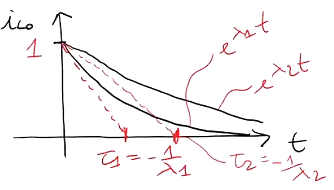
\includegraphics[width=0.4\linewidth]{evoluzione_libera_reali_distinte}
\end{figure}


\item Caso 2, radici reali e coincidenti, caso piuttosto patologico
la radice viene determinata con $-\sigma$ si avrà un modo esponenziale decrescente $e^{-\sigma t} $ con
$\tau = \frac{1}{\sigma}$ e un modo pari a  $t\cdot e^{-\sigma t}$
$$
i_{L_0} = K_1 e^{-\sigma t} + K_2 t\cdot e^{-\sigma t}
$$
\begin{figure}[H]
\centering
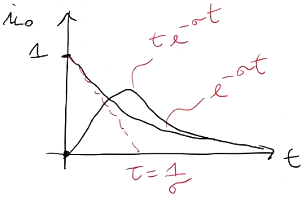
\includegraphics[width = 0.4\linewidth]{evoluzione_libera_reali_coincidenti}
\end{figure}
Vengono detti modi aperiodici smorzati con smorzamento critico.


\item Caso 3, modi periodici smorzati, soluzioni complesse coniugate
$\lambda_{1,2} = -\sigma \pm j\omega_d$, la distanza tra due picchi è pari a $\frac{2\pi}{\omega_d}$
$$i_{L_0}(t) = e^{-\sigma t} [K_1 \cos (\omega_d t) + K_2 \sin(\omega_d t)]$$
\begin{figure}[H]
\centering
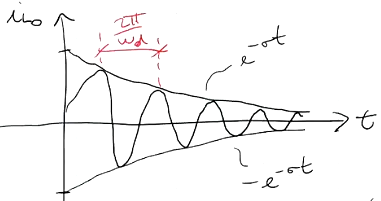
\includegraphics[width=0.4\linewidth]{evoluzione_libera_complesse_coniugate}
\end{figure}
\end{itemize}

Restano da determinare le costanti di integrazione imponendo le condizioni iniziali,
\begin{equation*}
\begin{cases}
i_L(0^+) = i_L(0^-) = \SI{0}{\ampere}\\
\frac{di_L}{dt}(0^+) = \frac{1}{L}[v_C(0^+) - R_2i_L(0^+)] = 0
\end{cases}
\end{equation*}

Supponendo dunque di avere soluzioni $\lambda_1,\ \lambda_2$ reali e distinte e ricordando di aggiungere
il termine a regime $\frac{E}{R_1 + R_2}$ nella determinazione dei coefficienti
$$
\begin{aligned}
i_L(0^+) = 0 & \Rightarrow \\
\frac{di_L}{dt}(0^+) = 0 & \Rightarrow
\end{aligned}
\begin{cases}
K_1+K_2 + \frac{E}{R_1+R_2} = 0 \\
\lambda_1K_1 + \lambda_2K_2 = 0
\end{cases}
$$
La soluzione del sistema permette di ricavare i coefficienti $K_1$ e $K_2$

%Lezione 2 i minuti si riferiranno a quelli visibili su teams e non quelli del file registrato con OBS
\section{Determinazione equazioni di stato di un circuito qualsiasi}

Si riprende la classe di circuiti lineari tempo invarianti (LTI), supponiamo di conoscere
le variabili di stato $i_L(t) $ e $v_C(t) $ assumendole note, sostituiamo ogni \textit{condensatore}
con un generatore di tensione di valore pari alla $v_C(t)$ , ripetendo il procedimento
per ciascun \textit{induttore} che viene sostituito con un generatore di corrente con corrente impressa
pari a $i_L(t)$.

In queste condizioni, la soluzione del circuito resta formalmente invariata.
Il nuovo circuito sarà di tipo adinamico, non presenterà più alcun componente dinamico, il nuovo circuito
prende il nome di \textit{circuito resistivo associato al circuito di partenza}.

Il vantaggio di questa operazione è la possibilità di ricavare $v_L$ e $i_C$ utilizzando il principio
di \textit{sovrapposizione degli effetti} (PSE).

Si ricavano le equazioni di stato per il seguente circuito:
26:07

\begin{figure}[h]

\end{figure}

Si applica il PSE, per trovare $i_C$ e $v_L$:
$$
i_C = i_c' + i_C'' + i_C '''
$$
$$
v_L = v_L' + v_L'' + v_L'''
$$

Disegna circuiti 28:48

Circuito 1)
$$
v_L' = 0;\ i_C' = \frac{E}{R_1} 
$$
Circuito 2)
$$
i_C'' = -\frac{v_C}{R_1};\ v_L'' = v_C
$$
Circuito 3)
$$
i_C''' = -i_L;\ v_L''' = -R_2\cdot i_L
$$

Sommando i tre contributi:
$$
i_C = \frac{E}{R_1} - \frac{v_C}{R_1} - i_L = C\frac{dv_C}{dt}
$$
$$
v_L = v_C - R_2\cdot i_L = L\frac{di_L}{dt}
$$
con le condizioni di continuità delle variabili di stato:
$$
i_L(0^+) = i_L(0^-)
$$
$$
v_C(0^+) = v_C(0^-)
$$

\section{Circuiti lineari con generazioni impulsivi}
Si analizza ora un circuito che presenta generatori di tipo impulsivo, ad esempio la risposta di 
una linea elettrica a seguito di una fulminazione.
Si definisce quindi l'impulso rettangolare di ammpiezza $\Delta$, la funzione viene chiamata 
$\Pi_\Delta(t)$,(funzione porta) è costante nell'intervallo $[-\frac{\Delta}{2},\frac{\Delta}{2}]$,
l'area del rettangoloide sotteso alla funzione è pari a
$$
\int_{-\Delta/2}^{\Delta/2}\Pi_\Delta(\tau)d\tau = 1\ \forall\ \Delta \in\ ]0,+\infty[
$$
Ha senso considerare la successione di funzioni ottenute per valori $\Delta$ decrescenti,
ma dimezzando la base, per mantenere l'area unitaria, va raddoppiata l'altezza.

Passando al limite per $\Delta \rightarrow 0^+$ la successione tende in maniera non ordinaria
ad un limite che non è una funzione ma può essere definita come funzione generalizzata,
ossia distribuzione, che prende il nome di \textbf{Delta di Dirac} ($\delta(t)$).

Proprietà della delta:
\begin{itemize}
\item È nulla $\forall t \neq 0$
\item Ha integrale unitario
\item Proprietà di campionamento $\int_{-\infty}^{+\infty}f(\tau)\delta(\tau-t_0)d\tau = f(t_0)$
\end{itemize}
Esempio della proprietà di campionamento: 49:03
$$
\int_{-\Delta/2}^{\Delta/2} f(\tau)\Pi_\delta(\tau-t_0)d\tau = \frac{1}{\Delta} \int_{-\Delta/2}^{\Delta/2}  f(\tau)d\tau = f(\vartheta^*)
$$


Analizziamo un'altra funzione $U_\Delta(t)$ definita come segue:
\begin{equation*}
\begin{cases}
0\ ,& t  < -\frac{\Delta}{2} \\
1\ ,& t  > \frac{\Delta}{2} \\
\frac{1}{2}+\frac{t}{\Delta}\ ,& -\frac{\Delta}{2} \leq t \leq \frac{\delta}{2}
\end{cases}
\end{equation*}
Rampa 55:03

Eseguendo la derivata temporale si otterrà la funzione $\Pi_\Delta(t)$, al limite di $\Delta \rightarrow 0$
si ottiene la funzione definita ``gradino'' o funzione di Heaviside $u(t)$.

Un ulteriore modo per definire la $\delta(t)$ è appunto quella di derivata della funzione gradino $u(t)$.
$$
\delta(t) = \frac{d}{dt}u(t) \Leftrightarrow \int_{-\infty}^t \delta(\tau)d\tau = u(t)
$$

\paragraph{Esempio con generatore impulsivo}
Si prenda un circuito RC serie 01:12:00 e una funzione $e(t)$ che vale $E_0$ per $0 < t < T$ e $0$ 
altrimenti.
Ricaviamo $v_C(t)$:

Si suppone che la condizione iniziale, ossia per $t < 0 $, la tensione sul condensatore sia nulla.

\begin{equation*}
\begin{cases}
e(t) &= RC\frac{dv_C}{dt} + v_C \\
v_C(0) &= 0
\end{cases}
\end{equation*}

$$
\begin{cases}
E_0 &= RC\frac{dv_C}{dt} + v_C \\
v_C^{(1)}(0) &= 0 \\
0 \leq t \leq T
\end{cases}
$$

$$
\begin{cases}
0 &= RC\frac{dv_C}{dt} + v_C \\
v_C^{(2)}(0) &= v_C^{(1)}(T) \\
t \geq T
\end{cases}
$$
Rivedi 1:19:00

Si ottiene una funzione esponenziale crescente fino a $T$ e poi decrescente fino a 0 all'infinito.
Diminuendo il valore di $T$ si vede che il ``picco'' della funzione sarà più basso, al limite 
di $T \rightarrow 0$ la soluzione si annulla.
Se imponiamo il prodotto $E_0\cdot T = 1$ ed eseguiamo il limite invece:
$$
\lim_{T\rightarrow0^+} v_C(t)
$$
Supponiamo di sviluppare la funzione esponenziale con la sua serie di Taylor:
$$
e^x = 1 + x + \frac{x^2}{2!} + \frac{x^3}{3!} + ... \Rightarrow 1-e^{-\frac{t}{\tau}} \simeq \frac{t}{\tau} 
$$

$$
\begin{cases}
0\ & t\leq 0 \\
\frac{1}{T}\frac{t}{\tau}\  & 0 \leq t\leq T \\
\frac{1}{T}\frac{T}{\tau} e^{-\frac{t-T}{\tau}}\ & t\geq T
\end{cases}
$$
Per $T\rightarrow 0^+$
$$
\begin{cases}
0\ & t\leq 0\\
\frac{1}{\tau}e^{\frac{-t}{\tau}}\ & t \geq 0
\end{cases}
$$

Il primo tratto dell'equazione si approssima quindi ad un tratto lineare fino a T, arrivando ad 
un'altezza di $\frac{1}{\tau}$ vedi figura 1:32:00

Se 
$$\Pi_\Delta(t) \stackrel{\Delta\rightarrow0^+}{\rightarrow} \delta(t) \Rightarrow v_C(t) \rightarrow h(t)$$
$h(t)$ è chiamata risposta all'impulso del circuito dinamico.

$$
\delta(t) = RC\frac{dv_C}{dt} + v_C \Leftarrow i_C = \frac{\delta(t)-v_C}{R}
$$
Se la tensione è impulsiva anche la corrente nel condensatore sarà di tipo impulsivo
$$
i_c = C\frac{dv_C}{dt} \Rightarrow \int_{0^-}^{0^+} i_C(\tau)d\tau = e[v_C(0^+)-v_C(0^-)]
$$
$$
v_C(0^+) - v_C(0^-) = \frac{1}{RC} \int_{0^-}^{0^+} \delta(\tau)d\tau - \frac{1}{RC} \int_{0^-}^{0^+} v_C(\tau)d\tau = \frac{1}{RC} = \frac{1}{\tau} \Rightarrow 
$$
$$
\Rightarrow v_C(0^+) = \frac{1}{RC} = \frac{1}{\tau}
$$
Rivedi discorso potenza 1:44:00

\paragraph{Risposta al gradino unitario di un circuito dinamico LTI}
Stesso circuito del precedente, ma stavolta si utilizza come forzamento il gradino unitario di
Heaviside, la soluzione è più semplice della precedente:

$$
v_C(t) = 1-e^{-\frac{t}{\tau}}u(t)
$$
la chiamiamo $g(t)$ e affermiamo che sia la risposta al gradino, richiamiamo la relazione
tra la funzione $\Pi_\Delta(t)$ e $U_\Delta(t)$ si ha che:
$$
\Pi_\Delta(t) = \frac{U_\Delta\left(t+\frac{\Delta}{2}\right)-U_\Delta\left(t-\frac{\Delta}{2}\right)}{\Delta} = e(t)
$$
per $\Delta \rightarrow 0^+$ ottengo $h(t) = v_C(t)$.

Essendo il circuito tempo invariante, si può trovare la risposta alla funzione $\Pi_\Delta(t)$
come combinazione lineare delle risposte delle due $U_\Delta$ opportunamente traslate, ossia
la risposta al gradino traslata.
$$
\text{Risp} \Pi_\Delta(t) = \frac{\text{Risp}\left\{U_\Delta\left(t+\frac{\Delta}{2}\right)\right\} - 
\text{Risp}\left\{U_\Delta\left(t-\frac{\Delta}{2}\right)\right\}}{\Delta} = 
\frac{g\left(t+\frac{\Delta}{2}\right) - g\left(t-\frac{\Delta}{2}\right)}{\Delta}
$$
Tutto si trasforma nella funzione rapporto incrementale della funzione $g(t)$ ossia
$$
\lim_{\Delta\rightarrow0^+}\text{Risp}\left\{\Pi_\Delta(t)\right\} = h(t) = \frac{dg}{dt}
$$

$$
h(t) = \frac{dg}{dt} = 0,\ t < 0;\ \frac{1}{\tau}e^{-\frac{t}{\tau}},\ t\geq0 
$$
La risposta all'impulso è quindi la derivata della risposta al gradino.

Si consideri un circuito RC serie
\begin{figure}[H]\centering
\begin{circuitikz}
\draw
(0,0) to [voltage source,invert,l=$u(t)$] (0,2)
      to [R=$R$] (2,2)
      to [C,l_=$C$,v^=$v_C$] (2,0) -- (0,0)
;
\end{circuitikz}
\end{figure}
si suppone che la tensione imposta al generatore sia un gradino unitario $u(t)$,
l'equazione di stato sarà:
$$
\begin{cases}
u(t) = RC \frac{dv_C}{dt} + v_C \\
v_C(0^+) = 0
\end{cases}
\Rightarrow v_C(t) = \left.
\begin{cases}
0 & t<0 \\
1-e^{-\frac{t}{\tau}} & t\geq 0
\end{cases}\right] = g(t)
$$

Si considera la funzione $U_\Delta$
$$U_\Delta(t) = 
\begin{cases}
0 & t< -\frac{\Delta}{2}\\
\frac{1}{2} + \frac{t}{\Delta} & -\frac{\Delta}{2} < t < \frac{\Delta}{2} \\
1 & t > \frac{\Delta}{2}
\end{cases}
$$
se si esegue la differenza di due funzioni $U_\Delta$ traslate di $\pm\frac{\Delta}{2}$ si ottiene 
una porta trapezoidale
$$
f(t) = \frac{U_\Delta\left(t+\frac{\Delta}{2}\right) - U_\Delta\left(t-\frac{\Delta}{2}\right)}{\Delta}
$$
tende ad una $\delta(t)$ delta di Dirac per $\Delta \rightarrow 0$.
Semplicemente si può invece definire la porta come differenza di due gradini traslati, in questo modo
si elimina il problema dei segmenti obliqui.

La linearità del sistema e la tempo-invarianza delle grandezze dei bipoli implica che la
risposta ad una combinazione lineare di funzioni traslate nel tempo si ottiene come combinazione lineare 
delle risposte dei singoli termini traslati.
$$
\text{Risp}\left\{\Pi_\Delta(t)\right\} = \frac{\text{Risp}\left\{u\left(t+\frac{\Delta}{2}\right) \right\} -\text{Risp}\left\{ u\left(t-\frac{\Delta}{2}\right) \right\}}{\Delta} = \frac{g\left(t+\frac{\Delta}{2}\right)-
g\left(t-\frac{\Delta}{2}\right)}{\Delta}
$$
Eseguendo il limite per $\Delta\to 0^+ $ si vede che quello appena presentato è un rapporto incrementale e
quindi
$$
\lim_{\Delta\to0^+} \Rightarrow \text{Risp} \left\{\delta(t)\right\} =h(t) = \frac{dg}{dt}
$$
Ricordando le funzioni $h(t)$ e $g(t)$ si vede la relazione
$$
h(t) = \begin{cases}
0 & t<0\\
\frac{1}{\tau}e^{-\frac{t}{\tau}} & t\geq 0
\end{cases}\qquad
g(t) = \begin{cases}
0 & t<0\\
1 - e^{-\frac{t}{\tau}} & t\geq 0
\end{cases} \Rightarrow
\frac{dg}{dt} = h(t)
$$
è possibile studiare la risposta all'impulso sfruttando quella al gradino, che è una funzione limitata e 
più semplice da analizzare.

\paragraph{Circuiti RC ed RL semplici con generatori impulsivi}
Si considerino 2 circuiti modello: il circuito RC parallelo e il circuito RL serie.

\begin{figure}[H]\centering
\begin{subfigure}{.4\textwidth}\centering
\begin{circuitikz}
\draw
(0,0) to [current source,l=$j(t)$] (0,2)
      to (1,2) to [R=$R$,i>^=$i_R$] (1,0) to (0,0);
\draw
(1,2) to (2.5,2)  to [C,l_=$C$,v^=$v_C(t)$,i>_=$i_C$] (2.5,0) -- (1,0)
;
\end{circuitikz}
\subcaption{RC parallelo}
\end{subfigure}
\begin{subfigure}{.4\textwidth}\centering
\begin{circuitikz}
\draw
(0,0) to [voltage source,invert,l=$e(t)$] (0,2)
      to [R,l_=$R$] (2.5,2) to [L,l_=$L$,i_>=$i_L(t)$,v^=$v_L$] (2.5,0) -- (0,0)
;
\end{circuitikz}
\subcaption{RL serie}
\end{subfigure}
\end{figure}

Siano i generatori impulsivi: $j(t) = Q\delta(t)$ ed $e(t) = \Phi\delta(t)$.
$$
j(t) = \frac{v_C}{R} + i_C = Q\delta(t) = \frac{v_C}{R} + C\frac{dv_C}{dt}
$$
Si integra la funzione nell'istante in cui è centrata la $\delta(t)$ ossia:
$$
\int_{0^-}^{0^+} Q\delta(\tau)d\tau  = \cancel{\int_{0^-}^{0^+}\frac{v_C}{R}d\tau} + C[v_C(0^+)-\cancel{v_C(0^-)}]
\Leftrightarrow Q = Cv_C(0^+) \ \ [Q] = \si{\coulomb} \text{ (Coulomb)}
$$
$$
\left[\int_{0^-}^{0^+} Q\delta(\tau)d\tau\right] = \text{ Coulomb}
$$
Tirando la costante $C$ fuori dall'integrale, che ha la dimensione di Coulomb, l'integrale rimanente
deve essere adimensionale.
Ciò significa che la $\delta(t)$ ha la dimensione di \si{\per\second} per essere coerente con l'integrale
e restituire una quantità finita.

\subparagraph{Caso duale con circuito RL:}

$$
e(t) = R\cdot i_L + v_L
$$
$$
\Phi\delta(t) = R\cdot i_L + L\frac{di_L}{dt}
$$
$$
\Phi\int_{0^-}^{0^+} \delta(\tau)d\tau = L i_L(0^+)\ , \ i_L(0^-) = 0
$$

Anche in questo caso per avere la dimensione del flusso in \si{\weber} per $\Phi$ allora la $\delta(t)$ 
avrà le dimensioni di \si{\per\second}.
\newpage
\subsection{Procedura generale per la risoluzione di circuiti con generatori impulsivi}
Si ha un circuito dinamico semplice al quale è collegato un generatore impulsivo,
si determina il circuito resistivo associato, ossia vengono sostituiti i condensatori con 
generatori di tensione e gli induttori con generatori di corrente.

Si ottiene un circuito parziale in cui si spengono i generatori interni (anche quelli equivalenti ai bipoli dinamici) e si lascia agire solo il generatore impulsivo.

Un ulteriore circuito è ottenuto facendo l'esatto contrario e spegnendo quindi il generatore impulsivo.

\begin{figure}[H]\centering
\begin{subfigure}{0.45\linewidth}\centering
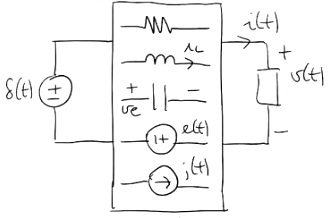
\includegraphics[width=\linewidth]{lezione_03_circuito_A}
\subcaption{Circuito iniziale}
\end{subfigure}
\begin{subfigure}{0.45\linewidth}\centering
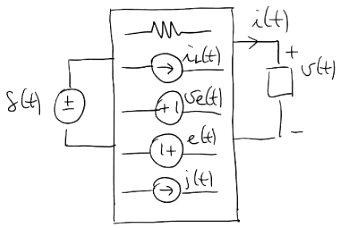
\includegraphics[width=\linewidth]{lezione_03_circuito_B}
\subcaption{Circuito resistivo associato}
\end{subfigure}
\begin{subfigure}{0.45\linewidth}\centering
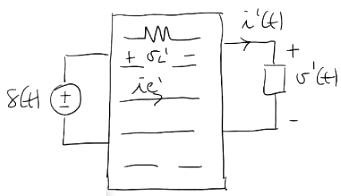
\includegraphics[width=\linewidth]{lezione_03_circuito_C-}
\subcaption{Circuito C'}
\end{subfigure}
\begin{subfigure}{0.4\linewidth}\centering
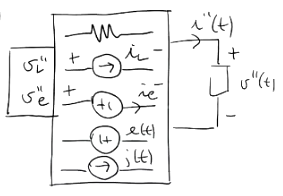
\includegraphics[width=\linewidth]{lezione_03_circuito_C--}
\subcaption{Circuito C"}
\end{subfigure}
\end{figure}
37:19
Si applica il PSE (Principio di Sovrapposizione degli effetti)
$$
\begin{cases}
v_L = v_L' + v_L''\\
i_C = i_C' + i_C''
\end{cases}
$$

Dal circuito C' si ricavano $v_L'$ e $i_C'$ causate dai generatori impulsivi 41:41

Viceversa dal circuito C'' si valutano le variabili di stato utilizzando come condizioni iniziali
le variabili ottenute in C'.

$$
v_C(0^+) = \frac{1}{C} \int_{0^-}^{0^+} i_C'(\tau)d\tau \ , \ v_C(0^-) = 0
$$
$$
i_L(0^+) = \frac{1}{L} \int_{0^-}^{0^+} i_L'(\tau)d\tau \ , \ i_L(0^-) = 0
$$
L'integrale delle variabili di stato del circuito C'' è pari a 0 dato che la funzione integranda è limitata
e l'intervallo è infinitesimo.

Infine si risolve il circuito C'' usando le variabili di stato appena calcolate in C'.

Esercizio 

Conclusione dell'esercizio: le variabili di stato possono essere discontinue ma limitate, le altre
variabili possono invece essere anche impulsive.

\paragraph{Risposta forzata di un circuito LTI}
Si suppone di avere un solo generatore esterno, se ne vogliono determinare le variabili ai capi
di un solo bipolo, si parla di filtro o sistema SISO \textit{(Single Input Single Output)},
sia $x(t)$ l'ingresso e $y(t)$ l'uscita, si deve supporre che il circuito sia a stato 0, ossia
le sue variabili di stato sono tutte nulle (circuito precedentemente spento).

Si parla di approssimazione \textit{PieceWise-Constant} ossia costante a tratti dell'ingresso
$x(t)$.
Si partiziona l'asse dei tempi in tanti intervalli di ampiezza $\Delta t$ centrati negli istanti
di tempo $t_k = k\Delta t\ ,\ k\ \in\ Z$.

Costruiamo un'approssimazione $x_\Delta(t)$ costante di valore $x(t_k)$ in $\left[t_k-\frac{\Delta t}{2}\ ,\ 
t_k+\frac{\Delta t}{2}\right]$.
La funzione $x(t)$ può quindi essere rappresentata come somma di impulsi rettangolari successivi,
sfruttando la funzione $\Pi_{\Delta}(t)$, sarà quindi:
$$
x_{\Delta}(t) = \sum_{k = -\infty}^{+\infty} x(t_k) \Pi_\Delta(t-t_k)\Delta t
$$
Eseguendo il limite per $\Delta t \rightarrow 0^+$ in ipotesi di sufficiente regolarità:
$$
\lim_{\Delta t \to 0^+} x_\Delta(t) = x(t) = \int_{-\infty}^{+\infty} x(\tau) \delta (t-\tau)
d\tau
$$
Questa conclusione richiama la proprietà di campionamento della $\delta(t)$.

Se vogliamo calcolare la risposta di $x(t)$ allora:
$$
\text{Risp}\left\{x(t)\right\} = y(t) = \text{Risp} \left\{\int_{-\infty}^{+\infty} x(\tau)\delta(t-\tau)
d\tau\right\}
$$
per linearità e tempo-invarianza si ottiene
$$
y(t) = \int_{-\infty}^{+\infty} x(\tau)h(t-\tau) d\tau
$$
chiamato integrale di convoluzione, $h(t)$ è la risposta impulsiva per la variabile di uscita.

Si parla di prodotto di convoluzione tra due funzioni $f,g \ \in\ R$
$$
f * g(t) = \int_{-\infty}^{+\infty} f(\tau)g(t-\tau)d\tau
$$
Si può calcolare la risposta impulsiva... rivedi 1:57:00


Data la risposta all'ingresso impulsivo, si può calcolare la risposta a qualsiasi ingresso, mediante
l'uso dell'integrale di convoluzione.
Osservando attentamente l'integrale si vede che la risposta impulsiva gode della proprietà per la quale
$$
h(t) = 0 \ t<0,\ h(t) \neq 0 \forall t\ \geq 0 \Rightarrow t - \tau \geq 0 \Rightarrow \tau \leq t
$$

Se l'ingresso $x(t) = 0,\ t< t_0$ allora possiamo affermare che la $y(t)$ avrà come estremi di integrazione
$t_0^-$ e $t$, con il - si sottintende la possibilità che siano presenti $\delta(t_0)$ in quell'istante 
di tempo.

\paragraph{Esempi dell'utilizzo dell'integrale di convoluzione}
Circuito RC parallelo con forzamento esponenziale, forzato da un generatore di corrente.
$$
j(t) = I e ^{\frac{t}{\tau}} u(t)
$$
Per studiare la risposta del circuito bisogna per prima cosa determinare la $V_{cf}(t)$, mediante
lo studio della risposta impulsiva.
Per determinare la risposta impulsiva si forza il circuito con una $\delta(t)$, utilizzando i metodi 
precedenti.

$i_c = \delta(t)$
$$
v_c(0^+) = \frac{1}{C}\int_{0^-}^{0^+} i_c(\tau)d\tau + V_c(0^-) = \frac{1}{C}
$$
Per determinare la risposta impulsiva si determina l'evoluzione libera spegnendo il generatore,
ci sarà un parallelo RC con la seguente equazione di stato:
$$
\begin{cases}
RC\frac{dV_c}{dt} + v_C = 0 \\
V_c(0^+) = \frac{1}{C}
\end{cases}
$$
Quindi 
$$
V_{c_{lib}} = h(t) = \frac{1}{C} e^{-\frac{t}{RC}},\ t\geq 0
$$
$$
h(t) = \frac{1}{C}e^{-\frac{t}{RC}}\cdot u(t) \forall t
$$

Utilizzando l'integrale di convoluzione per calcolare la risposta forzata:

$$
V_{cf}(t) = \int_{0^-}^{t}Ie^{\frac{\tau}{T}} \cdot \frac{1}{C} e^{-\frac{t-\tau}{RC}} d\tau = 
\frac{I}{C} \int_{0^-}^{t} e^{\frac{\tau}{t}}\cdot e^{-\frac{t}{RC}}\cdot e^{\frac{\tau}{RC}} d\tau
$$

$$
= \frac{I}{C} e^{-\frac{t}{RC}}\cdot \frac{e^{t\left(\frac{1}{T}+\frac{1}{RC}\right)}-1}{\frac{1}{RC}+\frac{1}{T}}
$$

Circuito RC serie con forzamento in tensione a rampa lineare $e(t)$
$$
e(t) = \begin{cases}
0\ t<0 \\
\frac{t}{T},\ 0\leq t\leq T\\
0\ t>0
\end{cases}
$$
Possiamo rappresentare questa funzione mediante l'uso di due funzioni $u(t)$

$$
e(t) = \frac{t}{T}\left[u(t) - u(t-T)\right]
$$
Determiniamo quindi la risposta $h(t)$ mediante la risposta al gradino $g(t)$
Le equazione di stato è:
$$
\begin{cases}
1 = RC\frac{dV_c}{dt} + V_c \\
V_c(0) = 0 
\end{cases}
\Rightarrow V_c(t) = 1 - e^{-\frac{t}{RC}},\ t\geq 0$$
Quindi 
$$
g(t) = (1 - e^{-\frac{t}{RC}})u(t) \forall t
$$
ma
$$
h(t) = \frac{dg}{dt} = \frac{1}{RC}e^{-\frac{t}{RC}},\ t\geq 0
$$
Determiniamo ora la risposta forzata $v_{cf}(t)$:
$$
V_{cf}(t) = \int_{0^-}^{t} e(\tau) h(t-\tau)d\tau = \int_{0^-}^{t}\frac{\tau}{T}\left[u(\tau) - u(t-\tau)\right]
\cdot \frac{1}{RC} e ^{-\frac{t-\tau}{RC}}\cdot u(t-\tau)d\tau
$$
Svolgiamo ora l'integrale osservando che $e(\tau) \neq 0 $ solo se $t \in [0,T]$, separiamo quindi
il calcolo dell'integrale in due eventualità:
$$
t\leq T:\ \int_{0^-}^{t}\frac{\tau}{T}\frac{1}{RC}e^{-\frac{t-\tau}{RC}}d\tau = \frac{1}{TRC}e^{-\frac{t}{RC}}\int_{0^-}^{t}\tau e^{\frac{\tau}{RC}}d\tau 
$$
utilizzando l'integrazione per parti:
$$
\left(f\cdot g\right)' = f'g + g'f
$$
$$
f = \tau\ g' = e^{\frac{\tau}{RC}}
$$
$$
\frac{1}{TRC}e^{-\frac{t}{}RC}\int_{0^-}^{t}\frac{d}{dt}\left[\tau e^{\frac{\tau}{RC}}\cdot RC \right] -
RC e^{\frac{\tau}{RC}} d\tau =
$$
$$
\frac{1}{TRC} e^{-\frac{t}{RC}} \left\{ \left[t e^{\frac{t}{RC}}\cdot RC \right] - \left[(RC)^2 e^{\frac{\tau}{RC}} \right]_{0^-}^{t}  \right\} =
$$
$$
\frac{t}{T} - \frac{RC}{T}\left(1-e^{-\frac{t}{RC}}\right)
$$

Secondo caso:
$$
t > T:\ \int_{0^-}^{T} \frac{\tau}{T}\frac{1}{RC} e^{-\frac{t-\tau}{RC}}d\tau =  e^{-\frac{t-T}{RC}}-\frac{RC}{T}\left(e^{-\frac{t-T}{RC}} -e^{-\frac{t}{RC}} \right)
$$

\section{La trasformata di Laplace}
Il metodo dei fasori si basa sul concetto che conoscendo l'andamento di regime con grandezze isofrequenziali, si può risolvere il sistema traspotando le grandezze sinusoidali nel dominio simbolico
dei fasori, si rapprentano cioè le grandezze descrittive dei bipoli medianti numeri complessi.

Mediante la L-Trasformata si possono usare ancora una volta equazioni nel dominio complesso ma per 
studiare reti nel regime transitorio.

\paragraph{Analisi delle reti dinamiche LTI con Laplace}
Consideriamo un blocco contenenti tutte le equazioni circuitali nel dominio del tempo,
otteniamo tutte le equazioni di stato di induttori e condensatori.
Questo risultato si ottiene mediante i metodi di risoluzione delle ODE, per arrivare alla conoscenza
della dinamica delle \textit{variabili di stato}, se sono poi interessato ad altre variabili, attravarso
operazioni \textit{algebriche lineari} si conosce la dinamica di utte le variabili del circuito.

In alternativa, sfruttando la trasformata di Laplace, le equazioni ODE vengono trasformate nel dominio
di Laplace, saranno equazioni algebriche lineari anzichè differenziali, risolvendo quindi solo un sistema
di equazioni lineari si conosce direttamente la trasformata delle variabili di stato, effettuando quindi
il procedimento inverso di antitrasformazione si ricavano le variabili di stato nel dominio del tempo,
l'antitrasformazione può essere invece posticipata ed eseguita dopo aver ricavato le generiche variabili
del circuito, ancora una volta con operazioni algebriche.

La soluzione di un sistema di equazioni differenziali è notevolmente più complesso che risolvere un 
sistema lineare, ecco il vantaggio dell'utilizzo della trasformata di Laplace.

Definizione della trasformata di Laplace di una funzione $f(t)\ \in\ [0,+\infty[\to R$:
$$
L[f(t)] = F(s) = \int_{0^-}^{+\infty} f(t) e^{-st}dt \ F:s \in\ C \to C
$$
ammesso che l'integrale improprio converga, per assicurarci che ciò accade si pone la condizione sufficiente, verificata nella stragrande delle situazioni:
$$
\text{Se} \left|f(t) \right| \leq Me^{\alpha t} ,\ M,\alpha \in R \text{ costanti}
$$
allora l'integrale converge, dim.:
$$
\int_{0^-}^{+\infty} f(t) e^{-st}dt \leq \int_{0^-}^{+\infty} \left|f(t)\right| e^{-st}dt \leq
\int_{0^-}^{+\infty} Me^{\alpha t} e^{-st}dt = M\int_{0^-}^{+\infty} e^{(\alpha-s)t}dt
$$
condizione verificata per ogni $\Re \left\{ s\right\} > \alpha$.

Definizione dell'antitrasformata:
$$
L^{-1}\left[F(S) \right] = f(t) = \frac{1}{2\pi i} \lim_{T\to+\infty} \int_{\gamma-iT}^{\gamma+iT}
e^{st}F(s)ds
$$
con $\Re\left\{s\right\} = \gamma$ tale che tutte le singolarità di $F(s)$ si trovino a sinistra di $\gamma$.

\subsection{Proprietà della L-trasformata} Ricordando quelle utilizzate nel metodo dei fasori:
\begin{itemize}
\item Unicità: $\forall f(t) \in [0,+\infty[\ \exists!\ F(s) = L[F(s)]$

considerate $F(s)$ e $G(s)$, se $F(s) = G(s) \Rightarrow f(t) = g(t)$ quasi ovunque, ossia:
$$\int_{0^-}^{+\infty}|f(t) - g(t)|dt = 0$$

\item Linearità: date $f_1(t)$ ed $f_2(t) :\ [0,+\infty[ \rightarrow R,\ k_1,k_2 \in R$ allora
$$L[k_1f_1(t) + k_2f_2(t)] = k_1F_1(s) + k_2F_2(s) $$
si dimostra con la proprietà di linearità dell'integrale

\item Traslazione nel dominio di Laplace: sia data $f(t) \in [0^-,+\infty[,\ L[f(t)] = F(s)$ e
consideriamo $F(s-\lambda),\ \lambda\ \in\ C$ 
$$F(s-\lambda) = \int_{0^-}^{+\infty}f(t) e^{-(s-\lambda)t}dt = \int_{0^-}^{+\infty} (f(t)e^{\lambda t})e^{-st} dt \Rightarrow F(s-\lambda) = L[f(t) e^{\lambda t}]$$ con $\Re\{s\} > \lambda$ 

\item Derivazione: $f'(t)  = \frac{d}{dt}f(t),\ L[f(t)] = F(s)$ allora 
$$L\left[\frac{d}{dt}f(t)\right] = \int_{0^-}^{+\infty}f'e^{-st}dt \stackrel{\text{x parti}}{=} 
\left[fe^{-st}\right]_0^{+\infty} - \int_{0^-}^{+\infty}(-s)e^{-st}\cdot f dt =$$
$$= \left(\lim_{t\to\infty}\left[fe^{-st}\right]-f(0^-)\right) + sF(s) = sF(s) - f(0^-)$$
$$
L\left[\frac{d}{dt}f(t)\right] = sF(s) - f(0^-)
$$
\item Prodotto di convoluzione nel dominio di Laplace, facendo leva sul teorema di Borel:
$$
L\left[f*g(t)\right] =\int_{0^-}^{+\infty}\left(\int_{0^-}^{t}f(\tau)g(t-\tau)d\tau\right) e^{-st}dt = F(s)\cdot G(s)
$$
per dimostrare questo teorema si scambiano le variabili di integrazione $t$ e $\tau$ sfruttando i teoremi
di \href{https://it.wikipedia.org/wiki/Teorema_di_Fubini}{Fubini} e Tonelli
\end{itemize}
\newpage
Trasformate notevoli di frequente utilizzo nei circuiti:
\begin{itemize}
\item Esponenziale: $f(t) = e^{\lambda t},\ \lambda\ \in R $ 
$$
L\left[e^{\lambda t}\right] = \int_{0^-}^{+\infty} e^{-(s-\lambda) t} dt = \left[\frac{1}{\lambda -s}e^{(\lambda -s)t}\right]_{0^-}^{+\infty} = \frac{1}{\lambda -s} \left[\lim_{t\to\infty}e^{(\lambda-s)t}-1\right] =
\frac{1}{s-\lambda}
$$
\item Funzione gradino $u(t)$:
$$
L[u(t)] = \int_{0^-}^{+\infty}e^{0t}e^{-st}dt = \frac{1}{s}
$$
\item Delta di Dirac $\delta(t)$:
$$
L[\delta(t)] = \int_{0^-}^{+\infty}\delta(t) e^{-st}dt = e^{-s\cdot 0} = 1
$$
\item Funzioni sinusoidali, $\cos(\omega t)=\frac{e^{j\omega t}+e^{-j\omega t}}{2},\ \sin(\omega t) = \frac{e^{j\omega t}-e^{-j\omega t}}{2j}$
$$
L[\cos(\omega t)] = \frac{1}{2} L[e^{j\omega t}] + \frac{1}{2} L[e^{-j\omega t}] = \frac{s}{s^2+\omega^2},\ \Re\{s\} > 0
$$
$$
L[\sin(\omega t)] = \frac{1}{2j}\left(\frac{1}{s-j\omega}-\frac{1}{s+j\omega}\right) = \frac{\omega}{s^2+\omega^2},\ \Re\{ s\} > 0
$$
\end{itemize}


Funzioni generiche: $t\cdot f(t)$ con $f(t)$ le funzioni precedentemente analizzate.
\begin{itemize}
\item Esponenziale:
$$
L[te^{\lambda t}] = \int_{0^-}^{+\infty} t e^{\lambda t}e^{-s t} dt = \int_{0^-}^{+\infty}t e^{(\lambda -s)t}
dt = 
$$
$$
= \left[\frac{e^{(\lambda -s )t }}{\lambda-s}\cdot t\right]_{0^-}^{+\infty} - \int_{0^-}^{+\infty}1\cdot\frac{1}{\lambda -s}e^{(\lambda-s)t}dt = 
$$
$$
= 0 + \frac{1}{s-\lambda}\cdot\frac{1}{s-\lambda} = \frac{1}{s-\lambda} ,\ \Re\{s\} > \lambda
$$

\item Coseno:
$$
L[t\cos(\omega t)] = L\left[t \frac{e^{j\omega t}+e^{-j\omega t}}{2}\right] = \frac{1}{2}\frac{1}{(s-j\omega)^2} + \frac{1}{2}\frac{1}{(s+j\omega)^2} = 
$$
$$
= \frac{1}{2}\frac{1}{s^2-\omega^2-2j\omega s} + \frac{1}{2}\frac{1}{s^2-\omega^2+2j\omega s} =
\frac{1}{2}\frac{s^2-\omega^2+2j\omega s +s^2 -\omega^2 -2j\omega s}{(s^2-\omega^2)^2+4\omega^4s^2} =
$$
$$
= \frac{s^2-\omega^2}{(s^2+\omega^2)^2}
$$

\item Seno:
$$%%Rivedi il rigo qui sotto
L[t\sin(\omega t)] = \frac{1}{2j} \left[\frac{1}{(s-j\omega)^2}-\frac{1}{(s+j\omega)^2}\right] =
\frac{1}{2j}\left[\frac{s^2-\omega^2+2j\omega s-s^2+\omega^2+2j\omega s}{(s^2-\omega^2)^2+4\omega^2s^2}\right] = 
$$
$$
= \frac{2\omega s}{(s^2+\omega^2)^2}
$$
\item Funzioni che descrivono moti periodici smorzati, sfruttando la proprietà di traslazione
$f(t) = e^{-\sigma t}\cos(\omega t),\  e^{-\sigma t}\sin(\omega t)$:
$$
L[e^{-\sigma t}\cos(\omega t)] = L[\cos(\omega t)](s+\sigma) = \frac{s+\sigma}{(s+\sigma)^2+\omega^2}\ \Re\{s\} > -\sigma
$$
$$
L[e^{-\sigma t}\sin(\omega t)] = L[\sin(\omega t)](s+\sigma) = \frac{\omega}{(s+\sigma)^2+\omega^2}\ \Re\{s\} > -\sigma
$$
\end{itemize}
\newpage
\paragraph{Circuito RL serie con L-trasformata}
Sia dato il circuito RL serie, se ne voglia determinare la risposta impulsiva $h(t) = i_L(t)$ dato l'ingresso
$e(t) = \delta(t)$

\begin{figure}[H]
\centering
\begin{circuitikz}
\draw (0,0) to [voltage source,invert,l=$e(t)$] (0,2)  
            to  [R,l=$R$] (2,2) to [L,i>_=$i_L$,l_=$L$,v^=$v_L$] (2,0) to (0,0);
\end{circuitikz}
\end{figure}

$$
\begin{cases}
\delta(t) = R\cdot i_L + L\frac{di_L}{dt} \\
i_L(0^-) = 0
\end{cases}
$$
Si applica la trasformata di Laplace ad entrambi i membri della prima equazione, sfruttando anche
la proprietà di derivazione:
$$
1 = RI_L(s) + L(sI_L(s) - i_L(0^-))
$$
$$
L[i_L(t)] = I_L(s) = \frac{1}{R+sL} = \frac{1}{L}\frac{1}{\frac{R}{L}+s}
$$
L'antitrasformata sarà invece pari a:
$$
L^{-1}[I_L(s)] = \frac{1}{L} L^{-1}\left[\frac{1}{S+\frac{R}{L}}\right] = \frac{1}{L}e^{-\frac{t}{\tau}},\ 
\tau = \frac{L}{R}
$$

Si vede ora la risposta al gradino, $e(t) = u(t)$:
$$
u(t) = R\cdot i_L+ L\frac{di_L}{dt} \rightarrow \frac{1}{s} = RI_L + sLI_L 
$$
$$
I_L = \frac{1}{s(R+sL)} = \frac{A}{s} + \frac{B}{R+sL} = \frac{AR+sLA+sB}{s(R+sL)}
$$
Si ricavano i valori di $A$ e $B$ sfruttando il principio di identità dei polinomi:
$$\begin{cases}
LA+B = 0\\
AR = 1
\end{cases}$$

$$
A = \frac{1}{R},\ B = -\frac{L}{R}
$$
In conclusione:
$$
I_L(s) = \frac{1}{R}\left[\frac{1}{s}-\frac{L}{R+SL}\right] = \frac{1}{R}\left[\frac{1}{s}-
\frac{L}{L\left(\frac{R}{L}+s\right)}\right]
$$
Antitrasformando si ottiene:
$$
i_L(t) = \frac{u(t)}{R} - \frac{1}{R}e^{-\frac{R}{L}t}u(t) = \frac{u(t)}{R}\left(1-e^{-\frac{R}{L}}t\right)
$$

\subsection{Equazioni circuitali nel dominio della L-trasformata}
Si considera ancora la classe dei circuiti dinamici lineari tempo-invarianti (LTI),
nel dominio del tempo sono necessarie le LKT e le LKC, le caratteristiche dei bipoli e dei generatori.
Questo sistema è un DAE (Differential Algebric Equation), va trasformato in un ODE nelle variabili di stato per poter essere risolto.

Se si trasformano tutte le equazioni che provengono dalle leggi di Kirchhoff si ottengono ancora le stesse equazioni
ma nel dominio di Laplace:
$$
\sum_{k} (\pm)I_k(s) = 0
$$
$$
\sum_k (\pm)V_k(s) = 0
$$
Ancora le equazioni dei bipoli:
$$\begin{aligned}
V_R(s) &= RI_R(s)\\
V_L(s) &= sLI_L(s) - Li_L(0^-)\\
I_C(s) &= sCV_C(s) - Cv_C(0^-)\\
V_E(s) &= E(s)\\
I_J(s)&= J(s)
\end{aligned}$$

Per trattare i circuiti in evoluzione forzata ($i_L(0^-)=0,\ v_C(0^-)=0$) si può associare un'impedenza equivalente
ai bipoli, ad esempio l'impedenza operatoriale dell'induttore diventa
$$\begin{aligned}
Z_L(s) = sL,&\ V_L(s) = Z_LI_L(s)\\
Y_C(s) = sC,&\ I_C= Y_C V_C 
\end{aligned}$$
Questo risultato permette di utilizzare tutti i metodi precedentemente visti per la risoluzione
di un circuito, si esegue un'antitrasformazione alla fine per ritornare nel dominio del tempo.
Si è però posta l'ipotesi di trovarsi in evoluzione forzata, ossia supponendo uno stato iniziale 
nullo, cosa accade se ciò non è vero?

Stato non zero iniziale:
$$\begin{aligned}
V_L(s) &= sLI_L - L i_L(0^-)\\
V_L(s) &= Z_LI_L+E_0
\end{aligned}$$
Si modella il bipolo dinamico con un generatore di tensione in serie, impulsivo.
Si può fare un ragionamento simile con il condensatore al quale si affianca un generatore di corrente
in parallelo $J_{cc}$
$$\begin{aligned}
I_C(s) &= sCV_C(s) - Cv_C(0^-)\\
J_{cc} &= Cv_C(0^-)
\end{aligned}$$

\subsection{Funzione di trasferimento e legame con la risposta impulsiva}
Sia preso un generico circuito LTI, viene forzato con un generatore di tensione, se ne analizzano
le grandezze su un singolo bipolo interno al circuito, considerato quindi come un SISO $h(t)$,
l'uscita del sistema può essere calcolata mediante l'integrale di convoluzione della risposta impulsiva.
$$
y(t) = \int_{0^-}^{t} x(\tau)h(t-\tau)d\tau
$$
Si trasporta il fenomeno nel dominio di Laplace e si considera lo stesso circuito sostituito dai bipoli
operatoriali, si può ancora considerare il sistema come un SISO con ingresso pari a $X(s)$ e uscita
pari a $Y(s)$.
Questo circuito è a-dinamico lineare con un solo generatore, quindi tutte le grandezze sono proporzionali
al singolo forzamento, si può quindi affermare che $Y(s) = H(s)X(s)$ con $H(s)$ un coefficiente di 
proporzionalità.

$H(s)$ viene ricavato, mediante il teorema di Borel:
$$
L[f*g(t)] = F(s)\cdot G(s)
$$
$$
y(t) = \int_{0^-}^{t} x(\tau)h(t-\tau) d\tau \Rightarrow H(s) = L[h(t)]
$$
$H(s)$ si chiama quindi \textit{funzione di trasferimento} del circuito ed è definita come il rapporto
tra la trasformata dell'uscita e quella dell'ingresso e coincide con la trasformata della risposta
impulsiva del circuito:
$$
H(s) \stackrel{\text{def}}{=} \frac{Y(s)}{X(s)} = L[h(t)]
$$

\paragraph{Esempio} Circuito LC forzato in risonanza:

Si ha un generatore ideale di tensione, un induttore ideale e un condensatore ideale senza perdite,
questo circuito rappresenta il limite ideale 
La risonanza è associata ad una specifica pulsazione pari a:
$$
\omega_r = \frac{1}{\sqrt{LC}}
$$
e il forzamento è pari ad un segnale con pulsazione pari alla pulsazione di risonanza
$$
e(t) = E_m \sin(\omega_r t)
$$
Il circuito non può essere analizzato con il metodo dei fasori dato che non è dissipativo e l'energia 
immagazzinata nei bipoli dinamici non tende a 0 in evoluzione libera per $t\to \infty$.

Si utilizza quindi l'analisi nel dominio di Laplace:
$$
I(s) = \frac{E(s)}{sL+ \frac{1}{SC}}
$$
ma
$$
E(s) = \frac{\omega_r}{s^2+\omega_r^2} = \frac{\omega_r}{s^2+\frac{1}{LC}} = L[e(t)]
$$
$$
I(s) = \frac{E_m\omega_r s C}{(s^2+\frac{1}{LC})(s^2+\frac{1}{LC})} = \frac{E_m\omega_r\frac{sC}{LC}}{(s^2+\frac{1}{LC})^2} = \frac{E_m\omega_r}{L} \frac{s}{(s^2+\frac{1}{LC})^2}
$$
Riprendendo la trasformata del seno:
$$
L[t\sin(\omega_r t)] = \frac{2\omega s}{(s^2+\omega^2)^2}
$$
riprendendo il calcolo di $I(s)$:
$$
= \frac{E_m\omega_r}{2L\omega_r}\cdot \frac{2\omega_r s}{(s^2+\omega_r^2)^2} = \frac{E_m}{2L}\frac{2\omega_r s}{(s^2+\frac{1}{LC})^2}
$$
Antitrasformando:
$$
i(t) = L^{-1}[I(s)] = \frac{E_m}{2L} t \sin(\omega_r t)
$$

\newpage
\paragraph{Calcolo della funzione di trasferimento per un circuito del secondo ordine}

$$R_1 = \SI{5}{\ohm}\ R_2=R_3 = \SI{10} {\ohm}\ C=\SI{0.5}{\farad}\ L=\SI{1}{\henry}$$
\begin{figure}[H]\centering
\begin{circuitikz}
\draw (0,2) to [open,v=$e(t)$] (0,0); 
\draw (0,2) to [R,l_=$R_1$] (2,2)
            to [L,l_=$L$] (4,2)
            to [R,l_=$R_2$] (4,0) to (0,0);
\draw (4,2) to (7,2)
            to [R,l_=$R_3$,v^=$v(t)$] (7,0) to (4,0);
\draw (5.5,2) to [C,l_=$C$] (5.5,0);
\end{circuitikz}
\end{figure}
Si è interessati all'uscita $v(t)$ dato l'ingresso $e(t)$, ci si trasferisce ancora una volta dal 
dominio del tempo a quello di Laplace.
Si assegnano i parametri del circuito:
$R_1 = \SI{5}{\ohm}\ R_2=R_3=\SI{10}{\ohm}\ C =\SI{0.5}{\farad}\ L=\SI{1}{\henry} $
Sostituiti i bipoli con impedenze, si trovano la $Z_{eq}$ pari a $5 + s$ in serie con $\frac{1}{0.2+0.5s}$
La tensione in uscita sarà la partizione della tensione in ingresso tra queste due impedenze:
$$
V(s) = E(s)\frac{Z_{eq}^{(2)}}{Z_{eq}^{(2)}+Z_{eq}^{(1)}} = \frac{1}{(0.2+0.5 s)(\frac{1}{0.2+0.5 s}+5+s)} = \frac{1}{2+2.75+0.5s^2}
$$
Si trovano gli zeri del polinomio, saranno due radici reali e distinte,
la $H(s)$ sarà quindi:
$$
H(s) = \frac{k_1}{s+0.886} + \frac{k_2}{s+4.514} = \frac{k_1 5 +4.514 k_1 + k_2 s + 0.886 k_2 }{s^2+5.45+4} =
$$
$$
= \frac{2}{(s^2+5s+4)},\ 
\begin{cases}k_1+k_2 = 0\\
4.514k_1 + 0.886k_2 = 2
\end{cases}
$$
$$
k_1 = \frac{2}{4.514-0.886} = 0.551 = -k_2
$$
In conclusione 
$$
H(s) = \frac{0.551}{s+0.886} - \frac{0.551}{s+4.514}
$$
antitrasformando:
$$
L^{-1}[H(s)] = 0.551\left(e^{-0.886 t}-e^{-4.514 t}\right) = h(t)
$$


\subsection{Calcolo di antitrasformate di funzioni razionali}
Si supponga che nei circuiti siano presenti soltanto alcune tipologie di generatori, come ad esempio
generatori stazionari, sinusoidali... In queste ipotesi le trasformate di Laplace sono funzioni 
razionali, del tipo:
$$
F(s) = \frac{N(s)}{D(s)}\ N(s),D(s) \text{ polinomi con grado } n\leq d
$$

In generale la $F(s)$ è esprimibile come:
$$
F(s) = K + \frac{N^*(s)}{D(s)}\ K \text{ costante, } n^* < d
$$
la sua antitrasformata sarà:
$$
L^{-1}[F(s)] = k\delta(t) + L^{-1}\left[\frac{N^*(s)}{D(s)}\right] 
$$
per determinare la soluzione vanno ricercate le radici del denominatore, chiamate \textit{poli}
della funzione, mentre le radici del numeratore vengono chiamati \textit{zeri}.

La funzione può avere \textbf{poli semplici} di molteplicità 1:
$$
F^*(s) = \frac{k_1}{s-p_1} + \frac{k_2}{s-p_2} + ... + \frac{k_n}{s-p_n} = \sum_{i=1}^{N}\frac{k_i}{s-p_i}
$$
$k_i$ viene chiamato residuo i-esimo della $F^*(s)$ e si calcola con:
\begin{equation}
\lim_{s\to p_i} \left[(s-p_1)F^*(s)\right]
\label{eq:formula_poli_semplici}
\end{equation}

Esempio:
$$
F^*(s) = \frac{1}{0.5s^2+2.7s+2} = \frac{2}{s^2+5.4s+4} = \frac{k_1}{s+0.886} + \frac{k_2}{s+4.514}
$$
Applicando la \ref{eq:formula_poli_semplici}:
$$
k_1 = \frac{2}{-0.886+4.514} = 0.551
$$
Una volta trovati tutti i poli semplici, l'antitrasformata della funzione, diviene una somma di
antitrasformate dei singoli rapporti:
$$
L^{-1}[F^*(s)] = L^{-1}\left[\sum_{i=1}^{N}\frac{k_i}{s-p_i}\right] = \sum_{i=1}^{N} k_ie^{p_i t}
$$
\textbf{Poli multipli}, ossia con molteplicità maggiore di 1, si supponga ad esempio che $p_1$ sia un polo multiplo:
$$
F^*(s) = \frac{k_{11}}{(s-p_1)^2} + \frac{k_{12}}{s-p_1} + \sum_{i=3}^{N} \frac{k_i}{s-p_i}
$$
$$
k_{11} = \lim_{s\to p_1} \left[(s-p_1)^2F^*(s)\right]
$$
per determinare il secondo residuo del polo invece si deve eseguire il limite della derivata:
$$
k_{12} = \lim_{s\to p_1} \frac{d}{ds} \left[(s-p_1)^2 F^*(s)\right]
$$
Esempio:
$$
F^*(s) = \frac{2s+5}{(s+2)^2} = \frac{k_{11}}{(s+2)^2} + \frac{k_{12}}{s+2}
$$
$$
k_{11} = \lim_{s\to-2} \frac{(2s+5)\cancel{(s+2)^2}}{\cancel{(s+2)^2}} = 1
$$
$$
k_{12} = \lim_{s \to -2} \frac{d}{ds} [2s+5] = 2
$$
$$
F^*(s) = \frac{1}{(s+2)^2}+\frac{2}{s+2},\ L^{-1}[F^*(s)] = te^{-2t}+2e^{-2t}
$$

\textbf{Poli complessi e coniugati:}
Si trovano le radici del denominatore della seguente funzione:
$$
F^*(s) = \frac{2s-1}{s^2+4s+5} = \frac{k_1}{s+2+j} + \frac{k_2}{s+2-j}
$$
$$
k_1 = \frac{2(-2-j)-1}{\cancel{-2}-j\cancel{+2}-j} = \frac{-4-2j-1}{-2j} = \frac{5+2j}{2j} = 1 - \frac{5}{2}j
$$
$$
k_2 = \bar{k_1} = 1+\frac{5}{2}j
$$
$$
F^*(s) = \frac{1-\frac{5}{2}j}{s+2+j} + \frac{1+\frac{5}{2}j}{s+2-j}
$$
\\
$$
L^{-1}[F^*(s)] = \left(1-\frac{5}{2}j\right)e^{-(2+j)t} + \left(1+\frac{5}{2}j\right)e^{-(2-j)t} =
$$
$$
= \left(1-\frac{5}{2}j\right)e^{-2t}e^{-jt} + \left(1+\frac{5}{2}j\right)e^{-2t}e^{jt} =
$$
$$
= e^{-2t}\left[\frac{\left(e^{-jt}+e^{jt}\right)}{2}\cdot 2 - \frac{5}{2}je^{-jt}+\frac{5}{2}je^{jt}\right] =
$$
$$
= e^{-2t}\left[\frac{\left(e^{-jt}+e^{jt}\right)}{2}\cdot 2 + \frac{5}{2j}e^{-jt}-\frac{5}{2j}e^{jt}\right] =
$$
$$
= e^{-2t}\left[2\cos(t)-5\sin(t)\right]
$$
\newpage
\textbf{Esercizio 1 :}

Determinare la risposta all'impulso e al gradino
\begin{figure}[h]
\centering
\begin{circuitikz}
\draw (0,0) to [I,l=$j(t)$] (0,2)
            to (2,2) to [R,l_=$R$,i_=$i_R$] (2,0)
            to (0,0);
\draw (2,2) to (4,2) to [L,l_=$L$,i_=$i_L$] (4,0) to (2,0);
\draw (4,2) to (6,2) to [C,l_=$C$,v^=$v(t)$,i_=$i_C$] (6,0) to (4,0);
\end{circuitikz}
\caption{Circuito RLC parallelo}
\end{figure}
$$
R = \SI{10}{\kilo\ohm}\ L = \SI{100}{\milli\henry}\ C = \SI{10}{\micro\farad}
$$
$$
j(t) = u(t)
$$
$$
j(t) = \frac{v}{r} + i_L + i_C,\ v = L\frac{di_L}{dt},\ i_c = C\frac{dv_c}{dt}
$$
$$\begin{cases}
C\frac{dv_c}{dt} = i_c = u(t) -\frac{v}{r} - i_L\\
L\frac{di_L}{dt} = v(t)
\end{cases}
$$
Si risolve l'integrale generale esprimendo la $i_L$ in funzione della $v(t)$:
$$
L\frac{d}{dt}\left[u(t) -\frac{v}{r} - C \frac{dv}{dt}\right] = v(t)
$$
Dato che si esegue l'analisi per $t > 0$ la derivata di $u(t)$ è nulla.
$$
\begin{cases}
\frac{d^2v}{dt^2} + \frac{1}{RC}\frac{dv}{dt} + \frac{v}{LC} = 0\\
v(0^+)=0\\
\frac{dv}{dt}(0^+) = \frac{1}{C}\left[j(0^+) - \frac{v}{r}(0^+) - i_L(0^+)\right] = \frac{1}{C}
\end{cases}
$$
Si determinano ora le frequenze naturali del sistema:

$$
\lambda^2 + \frac{1}{RC}\lambda + \frac{1}{LC} = 0
$$
$$
\lambda_{1,2} = -\frac{1}{2RC} \pm \sqrt{\left(\frac{1}{2RC}\right)^2-\frac{1}{LC}}
$$
$$
\lambda^2 + \frac{1}{10^4\cdot10^{-5}}\lambda + \frac{1}{0.1\cdot10^{-5}} = 0
$$
$$
\lambda_{1,2} = -5 \pm j 1000
$$
Quindi si hanno modi naturali periodici smorzati ossia:
$$
v(t) = e^{-5t}(k_1\cos(1000t)+k_2\sin(1000t))
$$
Si impongono ora le condizioni iniziali:
$$
v(0^+) = 0 \Rightarrow k_1 = 0
$$
$$
\frac{dv}{dt}(0^+) = \frac{1}{C} \Rightarrow \left[-5e^{-5t}k_2\sin(1000t) + k_2e^{-5t}\cos(1000t)\cdot1000\right]_{t=0} = \frac{1}{C}
$$
$$
k_2\cdot1000 = \frac{1}{10^{-5}} \Rightarrow k_2 = 100
$$
$$
v(t) = 100e^{-5t}\sin(1000t)\cdot u(t) = g(t)
$$
Risposta all'impulso:
$$
h(t) = \frac{dg}{dt} = -500e^{-5t}\sin(1000t) + 100e^{-5t}\cdot1000\cdot\cos(1000t) = 
$$
$$
500e^{-5t}\left[200\cos(1000t)-\sin(1000t)\right]\cdot u(t)
$$
Verifica della $h(t)$, utilizzando la procedura per analizzare la risposta all'impulso, sostituendo
i bipoli dinamici, il condensatore diventerà un corto circuito e l'induttore un circuito aperto:
\begin{figure}[h]
\centering
\begin{circuitikz}
\draw (0,0) to [I,l=$\delta(t)$] (0,2)
            to (2,2) to [R,l_=$R$,i_=$i_R$] (2,0)
            to (0,0);
\draw (2,2) to (4,2) to [open,v_=$v_L$] (4,0) to (2,0);
\draw (4,2) to (6,2) to [short,i_=$i_C$] (6,0) to (4,0);
\end{circuitikz}
\caption{Circuito RLC con bipoli sostituiti}
\end{figure}

$i_C$ sarà chiaramente pari a $\delta(t)$ e $v_L = 0$.
Si determina la discontinuità di $v_C$:
$$
v_c(0^+) = \frac{1}{C}\int_{0^-}^{0^+}\delta(\tau)d\tau = \frac{1}{C}
$$
$$
i_L(0^+) = \frac{1}{L}\int_{0^-}^{0^+} v_L(\tau)d\tau = 0
$$
$$
\begin{cases}
v(0^+) = \frac{1}{C}\\
\frac{dv}{dt}(0^+) = \frac{1}{C}\left(-\frac{1}{RC}\right) = -\frac{1}{RC^2}
\end{cases}
$$
Le frequenze naturali sono le stesse, quindi l'equazione sarà dello stesso tipo: moto periodico smorzato
$$
v(0^+) = \frac{1}{C} = k_1 = 10^5
$$
$$
\frac{dv}{dt}(0^+) = 1000k_2 - \frac{5}{C} = -\frac{1}{RC^2} \Rightarrow 1000k_2 = \frac{5}{C} - \frac{1}{RC^2} = 5\cdot10^5 - \frac{10^{10}}{10^4} = 5\cdot10^5-10^6 = -5\cdot10^5
$$
$$
k_2 = -500
$$
In conclusione:
$$
h(t) = e^{-5t}\left[10^5\cos(1000t)-500\sin(1000t)\right] = 500e^{-5t}\left[200\cos(1000t)-\sin(1000t)\right]\cdot u(t)
$$

\textbf{Esercizio 2 :}
\begin{figure}[H]
\centering
\begin{circuitikz}
\draw (0,0) to [R,l=$R_1$] (0,2);
\draw (0,0) to (2,0) to [V,l=$e(t)$] (2,2) to (0,2);
\draw (2,2) to [C,l=$C$]  (4.5,2) to [L,l=$L$]  (4.5,0) to [R,l=$R_2$,v=$v(t)$]  (2,0);
\draw (4,2) to (6,2) to [R,l=$R_1$] (6,0) to (4,0);
\end{circuitikz}
\end{figure}

Si determini la risposta impulsiva nel dominio del tempo con la trasformata di Laplace
$$
R_1 = \SI{1}{\ohm},\ R_2 = \SI{3}{\ohm},\ L = \SI{3}{\henry},\ C = \SI{1}{\farad}
$$
Si determinano le condizioni iniziali dovute al generatore impulsivo $e(t) = \delta(t)$

%circuito ausiliario
\begin{figure}[h]
\centering
\begin{circuitikz}
\draw (0,0) to [R,l=$R_1$] (0,2);
\draw (0,0) to (2,0) to [V,l=$\delta(t)$] (2,2) to (0,2);
\draw (2,2) to [short,i=$i_C$]  (4.5,2) to [open,v=$v_L$]  (4.5,0) to [R,l=$R_2$,v=$v(t)$]  (2,0);
\draw (4,2) to (6,2) to [R,l=$R_1$] (6,0) to (4,0);
\end{circuitikz}
\caption{Circuito ausiliario}
\end{figure}
Si calcolano quindi le variabili di stato $v_L$ e $i_C$:
$$
v_L = -\frac{R_1}{R_1+R_2}\delta(t) = -\frac{1}{4}\delta(t)
$$
$$
i_C = -\frac{\delta(t)}{R_1+R_2} = -\frac{1}{4}\delta(t)
$$
$$
i_L(0^+) = \frac{1}{L} \int_{0^-}^{0^+} -\frac{\delta}{4}d\tau = \SI{-1/12}{\ampere} 
$$
$$
v_C(0^+) = \frac{1}{C} \int_{0^-}^{0^+}-\frac{\delta}{4}d\tau = -\frac{1}{4} = \SI{-0.25}{\volt}
$$
quindi
$$
v(t) = -\frac{R_2}{R_1+R_2}\delta(t) = -\frac{3}{4}\delta(t) = -0.75\cdot\delta(t)
$$

Si ricavano ora le equazioni di stato sfruttando le condizioni iniziali appena ricavate:

\begin{figure}[h]
\centering
\begin{circuitikz}
\draw (0,0) to [R,l=$R_1$] (0,2);
\draw (0,0) to (2,0) to [short] (2,2) to (0,2);
\draw (2,2) to [V,v=$v_C$,i^>=$i_C$]  (4.5,2) to [I,v>=$v_L$,l=$i_L$]  (4.5,0) to [R,l_=$R_2$,v^=$v(t)$]  (2,0);
\draw (4,2) to (6,2) to [R,l=$R_1$] (6,0) to (4,0);
\end{circuitikz}
\caption{Circuito resistivo associato}
\end{figure}
Applicando il principio di sovrapposizione degli effetti:
$$
\begin{cases}
i_c = -\frac{1}{R_1+R_2}v_C +\frac{R_1}{R_1+R_2}i_L = C\frac{dv_C}{dt}\\
v_L = -\frac{R_1}{R_1+R_2}v_C - \frac{R_1R_2}{R_1+R_2}i_L = L\frac{di_L}{dt}
\end{cases}
$$
Variabile di uscita:
$$
v(t) = R_2i_c = -\frac{R_2}{R_1+R_2}v_c + \frac{R_1R_2}{R_1+R_2}i_L = -\frac{3}{4}v_c +\frac{3}{4}i_L
$$

Riscrivendo ora la ODE in forma matriciale:
$$
\begin{pmatrix}
 C & 0 \\
 0 & L
\end{pmatrix}
\frac{d}{dt}
\begin{bmatrix}
v_c \\
i_L
\end{bmatrix}
=
\begin{bmatrix}
-\frac{1}{R_1+R_2} & \frac{R_1}{R_1+R_2}\\
-\frac{R_1}{R_1+R_2} & -\frac{R_1R_2}{R_1+R_2}
\end{bmatrix}\cdot
\begin{bmatrix}
v_c \\
i_L
\end{bmatrix}
$$
La forma matriciale generica è:
$$
D\frac{d\underline{x}}{dt} = A\underline{x}
$$
In questo caso la matrice A è l'opposta della matrice di rappresentazione ibrida del doppio bipolo visto 
dalle porte alle quali sono collegati i generatori $v_C$ e $i_L$.
$$
\underline{x}(t) = \underline{v}e^{\lambda t} \Rightarrow \lambda D \underline{v} e ^{\lambda t} = A\cdot \underline{v}e^{\lambda t} \Rightarrow A\cdot \underline{v} = \lambda D\cdot\underline{v}
$$
Quello appena citato è un problema agli autovalori generalizzato per le matrici $A$ e $D$.
$$
D^{-1}A\cdot\underline{v} = \lambda\underline{v} \Rightarrow D^{-1}A = 
\begin{bmatrix}
-\frac{1}{(R_1+R_2)C} & \frac{R_1}{(R_1+R_2)C} \\
-\frac{R_1}{L(R_1+R_2)} & -\frac{R_1R_2}{(R_1+R_2)L}
\end{bmatrix}
=
\begin{bmatrix}
-\frac{1}{4} & \frac{1}{4} \\
-\frac{1}{12} & -\frac{1}{4}
\end{bmatrix}
$$
Si calcolano quindi gli autovalori della matrice risolvendo il seguente problema:
$$
\text{det}\left(A-\lambda I\right) = 
\begin{vmatrix}
a_{11}-\lambda & a_{12}\\
a_{21} & a_{22}-\lambda
\end{vmatrix}
= (a_{11}-\lambda)(a_{22}-\lambda) -a_{12}a_{21} =
$$
$$
= a_{11}a_{22} - a_{11}\lambda - a_{22}\lambda + \lambda^2 - a_{12}a_{21} = \lambda^2 - tr(A) + det(A) =0
$$

$$
\lambda_{1,2} = -\frac{1}{4} \pm \sqrt{\frac{1}{16}+\left(\frac{1}{16}+\frac{1}{48}\right)} = -\frac{1}{4}\pm \frac{\sqrt{3}}{12} = - 0.25 \pm 0.1433j
$$
Si ha ancora una volta una soluzione sinusoidale smorzata
$$
v_c(t) = e^{-\sigma t}\left(k_1\cos(\omega t) + k_2\sin(\omega t)\right),\ \sigma = 0.25,\ \omega = 0.1443
$$
Si ricava direttamente anche la derivata in forma esplicita, necessaria al calcolo di $i_C$:
$$
\frac{dv_c}{dt}(t) = -\sigma e^{-\sigma t}\left(k_1\cos(\omega t)+k_2\sin(\omega t)\right) + e^{-\sigma t}(-k_1\omega \sin(\omega t) + k_2 \omega \cos(\omega t)) =
$$
$$
=e^{-\sigma t} \left[(k_2\omega -\sigma k_1)\cos(\omega t) - (\sigma k_2 + k_1\omega ) \sin(\omega t) \right]
$$
\begin{equation}
\frac{dv_c}{dt}(0^+)= -\sigma k_1 + \omega k_2
\label{eq:dvc_esercizio2}
\end{equation}

Imponendo le condizioni iniziali:
$$
v_c(0^+) = \SI{-0.25}{\volt} \Rightarrow k_1 = -0.25
$$
$$
\frac{dv_c}{dt}(0^+) = -\frac{1}{4}v_c(0^+) + \frac{1}{4}i_L(0^+) = \frac{1}{16} + \frac{1}{4}\left(\frac{1}{12}\right) = \frac{1}{24} = 0.0417
$$
usando la \ref{eq:dvc_esercizio2}
$$
-0.25 k_1 + 0.1443k_2 = 0.0417
$$
$$
k_2 = -\frac{\sqrt{3}}{12} = -0.1443
$$
In definitiva:
$$
v_c(t) = e^{-0.25 t}\left[-0.25\cos(0.1443 t) - \frac{\sqrt{3}}{12}\sin(0.1443 t)\right]
$$
Applicando l'equazione determinata dal circuito resistivo associato:
$$
v(t) = R_2 i_c - \frac{R_2}{R_1+R_2}\delta(t) = R_2C\frac{dv_c}{dt} - \frac{R_2}{R_1+R_2}\delta(t) =
3\frac{dv_c}{dt} - \frac{3}{4}\delta(t)=
$$
$$
= \frac{1}{8}e^{-\frac{1}{4}t}\left[\cos\left(\frac{\sqrt{3}}{12}t\right) + \sqrt{3}\sin\left(\frac{\sqrt{3}}{12}t\right)\right] - \frac{3}{4}\delta(t)
$$
$$
v(t) = 0.125 e^{-0.25 t}\left[\cos(0.1443 t) + 1.732\sin(0.1443 t)\right] - 0.75\cdot\delta(t)
$$
La variabile in uscita non essendo una variabile di stato può contenere, come in questo caso un valore 
impulsivo.
\newpage
\textbf{Soluzione con la L-trasformata}

Utilizzando le impedenze operatoriali
\begin{figure}[H]
\centering
\begin{circuitikz}
\draw (0,0) to [generic=$Z_{R1}$] (0,2) to (2,2) to [V,invert,l_=$V_s$] (2,0) to (0,0);
\draw (2,2) to [generic=$Z_C$] (4,2) to [generic=$Z_L$] (4,0) to [generic,l_=$Z_{R2}$,v^=$V$] (2,0);
\draw (4,2) to (6,2) to [generic=$Z_{R1}$] (6,0) to (4,0);
\end{circuitikz}
\end{figure}
$$
V = -V_s\frac{Z_{R2}}{Z_{R2}+Z_C+\frac{Z_L\cdot Z_{R1}}{Z_L+Z_{R1}}} = -V_s\frac{R_2}{R_2 + \frac{1}{sC} + 
\frac{sLR_1}{R_1+sL}} =
$$
$$
= -\frac{3}{3+\frac{1}{s} + \frac{3 s}{3s + 1}} = \frac{-3 s (3s + 1)}{3s(3s+1) + 3s+1 + 3s^2} = 
$$
$$
= \frac{- 3s(3s+1)}{12s^2+6s+1} = H(s)
$$
Antitrasformando $H(s)$:
$$
L^{-1}\left[\frac{-3s(3s+1)}{12s^2+6s +1}\right] = -3 \frac{d}{dt}L^{-1} \left[\frac{3s+1}{12s^2+6s+1}\right] = -\frac{1}{4} \frac{d}{dt} L^{-1} \left[\frac{3s+1}{s^2+0.5s + \frac{1}{12}}\right] =
$$
$$
= -\frac{1}{4} \frac{d}{dt} L^{-1}[F(s)]
$$
Decomponendo in fratti semplici:
$$
F(s) = \frac{k_1}{s+0.25+0.1443j} + \frac{k_2}{s+0.25-0.1443j}
$$
Si calcolano i residui eseguendo opportunamente i limiti con $p_1 = -0.25-0.1443j$ e $p_2$ il suo 
coniugato:
$$
k_1 = \frac{3p_1+1}{p_1-p_2} = \frac{3}{2}-\frac{\sqrt{3}}{2}j
$$  
$$
k_2 = \bar{k_1} = \frac{3}{2} +\frac{\sqrt{3}}{2}j
$$
Sostituendo:
$$
F(s) = \frac{\frac{3+\sqrt{3}j}{2}}{s + 0.25 + 0.1443j} + \frac{\frac{3-\sqrt{3}j}{2}}{s+0.25-0.1443j}
$$

La trasformata inversa viene eseguita con le funzioni esponenziali:
$$
L^{-1}[F(s)] = \frac{3+\sqrt{3}j}{2}e^{-0.25 t}e^{-j0.1443 t} + \frac{3-\sqrt{3}j}{2}e^{-0.25 t}e^{j0.1443 t}
$$
Raggruppando i termini:
$$
L^{-1}[F(s)] = e^{-0.125 t}\left[3\cos(0.1443 t) + \sqrt{3}\sin(0.1443 t)\right]\cdot u(t)
$$
$$
h(t) = -\frac{1}{4} \frac{d}{dt}L^{-1}[F(s)] = 0.125 e ^{-0.25 t}[\cos(0.1443 t) + \sqrt{3}\sin(0.1443 t)] - 0.75\cdot\delta(t)
$$
con $\delta(t) = \frac{d}{dt}u(t)$.


\section{Introduzione ai campi stazionari e instazionari}
\subsection{Richiami di analisi vettoriale}
\paragraph{Sistemi di riferimento e coordinate}
Per descrivere una proprietà nello spazio, si utilizza di solito un riferimento composto da 
una terna ortogonale di assi indicati con $L_1$ $L_2$ e $L_3$ con origine comune in $O$.
Si descrive un punto nello spazio $P$ con un raggio vettore che parte dall'origine e 
raggiunge il punto $P$.

\begin{figure}[h] %esempio punto P nello spazio
\centering
\begin{tikzpicture}[scale=3,tdplot_main_coords]
\draw [thick,->] (0,0,0) -- (1,0,0) node[anchor= north east]{$l_1$};
\draw [thick,->] (0,0,0) -- (0,1,0) node[anchor= north west]{$l_2$};
\draw [thick,->] (0,0,0) -- (0,0,1) node[anchor= south]{$l_3$};
\tdplotsetcoord{P}{0.8}{50}{45};
\coordinate (O) at (0,0,0);
\draw [-stealth,color=red] (O) -- (P) node[anchor = west]{$P$};

\draw [dashed,color=red] (O) -- (Px);
\draw [dashed,color=red] (O) -- (Py);
\draw [dashed,color=red] (O) -- (Pz);
\draw [dashed,color=red] (Px) node[anchor = south east]{$x$} -- (Pxy);
\draw [dashed,color=red] (Py) node[anchor = south west]{$y$} -- (Pxy);
%\draw [dashed,color=red] (Px) -- (Pxz);
%\draw [dashed,color=red] (Pz) -- (Pxz);
%\draw [dashed,color=red] (Py) -- (Pyz);
\draw [dashed,color=red] (O) -- (Pxy);
%\draw [dashed,color=red] (Pz) -- (Pyz);
\draw [dashed,color=red] (Pxy) -- (P);
%\draw [dashed,color=red] (Pxz) -- (P);
%\draw [dashed,color=red] (Pyz) -- (P);
\draw [dashed,color=red] (Pz) node[anchor = east]{$z$} -- (P);
\end{tikzpicture}
\end{figure}

Questo vettore può essere determinato con una terna di scalari $(u_1,u_2,u_3)$ che sono le 
coordinate del punto $P$.

La scelta più consona è quella di introdurre un sistema di coordinate cartesiane tali che 
$$
P \rightarrow (x,y,z)\ \ \vec{OP} = x\vec{e_x} + y\vec{e_y} + z\vec{e_z}
$$
con $\vec{e_x},\ \vec{e_y},\ \vec{e_z}$ i versori degli assi coordinati $l_1,\ l_2,\ l_3$.

In alternativa si possono utilizzare le coordinate \textbf{cilindriche}:

\begin{figure}[h] %esempio punto P coordinate cilindriche
\centering
\begin{tikzpicture}[scale=3,tdplot_main_coords]
\draw [thick,->] (0,0,0) -- (1,0,0) node[anchor= north east]{$l_1$};
\draw [thick,->] (0,0,0) -- (0,1,0) node[anchor= north west]{$l_2$};
\draw [thick,->] (0,0,0) -- (0,0,1) node[anchor= south]{$l_3$};
\tdplotsetcoord{P}{0.8}{50}{45};
\coordinate (O) at (0,0,0);
\draw [-stealth,color=red] (O) -- (P) node[anchor = west]{$P$};

\draw [color=red] (O) -- (Pxy) node[anchor = north]{$r$};
\tdplotdrawarc[color=blue,->]{(O)}{0.2}{0}{45}{anchor=north}{$\varphi$};
%\draw [dashed,color=red] (O) -- (Px);
%\draw [dashed,color=red] (O) -- (Py);
%\draw [dashed,color=red] (O) -- (Pz);
%\draw [dashed,color=red] (Px) node[anchor = south east]{$x$} -- (Pxy);
%\draw [dashed,color=red] (Py) node[anchor = south west]{$y$} -- (Pxy);
%\draw [dashed,color=red] (Px) -- (Pxz);
%\draw [dashed,color=red] (Pz) -- (Pxz);
%\draw [dashed,color=red] (Py) -- (Pyz);
%\draw [dashed,color=red] (Pz) -- (Pyz);
\draw [dashed,color=red] (Pxy) -- (P);
%\draw [dashed,color=red] (Pxz) -- (P);
%\draw [dashed,color=red] (Pyz) -- (P);
\draw [dashed,color=red] (Pz) node[anchor = east]{$z$} -- (P);
\end{tikzpicture}
\end{figure}

Il punto $P$ è ancora rappresentato da 3 scalari $(r,\varphi, z)$ e dato dalla combinazione di queste 
coordinate.
$$
\vec{OP} = r\vec{e_r} + \varphi\vec{e_{\varphi}} + z\vec{e_z}
$$

$$
\begin{cases}
r = \sqrt{x^2+y^2}\\
\sin\varphi = \frac{y}{\sqrt{x^2+y^2}},\ \cos\varphi = \frac{x}{\sqrt{x^2+y^2}}\\
z = z
\end{cases}
$$
Queste variabili possono essere ottenute in MATLAB con i seguenti comandi:
\verb|cart2pol| e $\varphi= $ \verb|atan2(y,x)| o viceversa \verb|pol2cart|.
$$
\begin{cases}
x = r\cos\varphi \\
y = r\sin\varphi \\
z = z
\end{cases}
$$

Un altro sistema di riferimento comunemente utilizzato è quello delle coordinate \textbf{sferiche}.

\begin{figure}[h] %esempio punto P coordinate sferiche
\centering
\begin{tikzpicture}[scale=3,tdplot_main_coords]
\draw [thick,->] (0,0,0) -- (1,0,0) node[anchor= north east]{$l_1$};
\draw [thick,->] (0,0,0) -- (0,1,0) node[anchor= north west]{$l_2$};
\draw [thick,->] (0,0,0) -- (0,0,1) node[anchor= south]{$l_3$};
\tdplotsetcoord{P}{0.8}{50}{45}; %coordinate punto P
\tdplotsetthetaplanecoords{45}; %coordinata phi per determinare il piano di theta
\tdplotdrawarc[tdplot_rotated_coords,color=blue,->]{(0,0,0)}{0.5}{0}{50}{anchor=south}{$\theta$};
\coordinate (O) at (0,0,0);
\draw [-stealth,color=red] (O) -- (P) node[anchor = west]{$P$};
\draw (0,0.18,0.13) node[color=red]{$r$};
\draw [dashed,color=red] (O) -- (Pxy);
\tdplotdrawarc[color=blue,->]{(O)}{0.2}{0}{45}{anchor=north}{$\varphi$};
%\draw [dashed,color=red] (O) -- (Px);
%\draw [dashed,color=red] (O) -- (Py);
%\draw [dashed,color=red] (O) -- (Pz);
%\draw [dashed,color=red] (Px) node[anchor = south east]{$x$} -- (Pxy);
%\draw [dashed,color=red] (Py) node[anchor = south west]{$y$} -- (Pxy);
%\draw [dashed,color=red] (Px) -- (Pxz);
%\draw [dashed,color=red] (Pz) -- (Pxz);
%\draw [dashed,color=red] (Py) -- (Pyz);
%\draw [dashed,color=red] (Pz) -- (Pyz);
\draw [dashed,color=red] (Pxy) -- (P);
%\draw [dashed,color=red] (Pxz) -- (P);
%\draw [dashed,color=red] (Pyz) -- (P);
%\draw [dashed,color=red] (Pz) node[anchor = east]{$z$} -- (P);
\end{tikzpicture}
\end{figure}

$$
P\rightarrow (r,\theta,\varphi)\ \ \vec{OP} = r\vec{e_r} + \theta\vec{e_\theta} + \varphi \vec{e_\varphi}
$$
con $(\vec{e_r},\vec{e_\theta},\vec{e_\varphi})$ terna levogira

$$
\begin{cases}
x = r\sin\theta\cos\varphi\\
y = r\sin\theta\sin\varphi\\
z = r\cos\theta
\end{cases}
$$
anche in questo caso è possibile utilizzare la funzione MATLAB \verb|sph2cart|.

Formule inverse:
$$
\begin{cases}
r &= \sqrt{x^2+y^2+z^2} \\
\cos\theta &= \frac{z}{\sqrt{x^2+y^2+z^2}}\\
\sin\theta &= \frac{\sqrt{x^2+y^2}}{\sqrt{x^2+y^2+z^2}} \\
\cos\varphi  &= \frac{x}{\sqrt{x^2+y^2}},\ \sin\varphi = \frac{y}{\sqrt{x^2+y^2}}
\end{cases}
$$

\subsection{Spostamenti elementari}
Supponiamo uno spostamento lungo la direzione $l_1$ associamo un coefficiente ``metrico'' pari 
alla distanza percorsa nel sistema di coordinate.

\begin{align*}
dl_1 &= h_1 du_1 \\
dl_2 &= h_2 du_2 \\
dl_3 &= h_3 du_3
\end{align*}

Questi fattori ``aggiustano'' le dimensioni delle relazioni in metri dovute a variazioni di 
coordinate differenti ad esempio in radianti.

Per le coordinate cartesiane i coefficienti metrici sono tutti uguali tra loro e pari ad 1.
$$
h_1 = h_2 = h_3 = 1 \Rightarrow
\begin{cases}
dl_1 = dx \\
dl_2 = dy \\
dl_3 = dz
\end{cases}
$$
Si suppone di costruire un volumetto elementare attorno il punto $P$, se ne può calcolare
l'area delle facce e il suo volume.
Si indica con $dS_1$ la superficie perpendicolare all'asse $l_1$, essa sarà pari a 
$dS_1 = dl_2\cdot dl_3 = dy\cdot dz$, si riportano per completezza le tre superfici:
\begin{align*}
dS_1 &= dl_2\cdot dl_3 = dy\cdot dz \\
dS_2 &= dl_3\cdot dl_1 = dz\cdot dx \\
dS_3 &= dl_1\cdot dl_2 = dx\cdot dy
\end{align*}
Il volume elementare invece si ricava con:
$$
dV = dl_1\cdot dl_2 \cdot dl_3 = dx\cdot dy\cdot dz
$$

Ripetiamo l'analisi per le \textbf{coordinate cilindriche:}
$ (u_1,u_2,u_3) = (r,\varphi,z)$

Supponiamo uno spostamento associato alla variazione della coordinata $r$, il raggio vettore
viene incrementato di una quantità $dr = dl_1 \Rightarrow h_1 =1$.

Effettuando una variazione $d\varphi$ invece il raggio vettore percorrerà un arco pari 
a $rd\varphi = dl_2 \Rightarrow h_2 = r$ per una variazione di arco ci sarà uno 
spostamento proporzionale alla distanza dall'origine $r$.
\begin{align*}
dr = dl_1 &\Rightarrow h_1 = 1\\
r d\varphi = dl_2 &\Rightarrow h_2 = r \\
dz = dl_3 &\Rightarrow h_3 = 1
\end{align*}
Superfici elementari:
\begin{align*}
dS_1 &= r\cdot d\varphi\cdot dz\\
dS_2 &= dz\cdot dr\\
dS_3 &= r\cdot dr\cdot d\varphi
\end{align*}
Volume infinitesimo:
$$
dV = r\cdot dr\cdot d\varphi\cdot dz
$$

In \textbf{coordinate sferiche} si ha $(u_1,u_2,u_3)=(r,\theta,\varphi)$

Ad una variazione $dr$ si ha uno spostamento lungo il raggio vettore $\vec{OP}$ quindi anche in questo
caso il fattore metrico sarà pari ad 1.

Ad una variazione della variabile $\theta$ detta anche co-latitudine, corrisponde una rotazione
pari a $dl_2 = r\cdot d\theta \Rightarrow h_2 = r$.

Ad una variazione di $\phi$ si ha un arco $dl_3 = r\cdot\sin\theta\cdot d \varphi \Rightarrow h_3 = r\cdot\sin\theta$
\begin{align*}
dl_1 &= dr & h_1 &=1 \\
dl_2 &= r\cdot d\theta & h_2 &=r \\
dl_3 &= r\cdot\sin\theta\cdot d\varphi & h_3 &= r\cdot \sin\theta 
\end{align*}

Superfici infinitesime:
\begin{align*}
dS_1 &= r^2\cdot\sin\theta\cdot d\theta\cdot d\varphi \\
dS_2 &= r\cdot \sin\theta \\
dS_3 &= r\cdot d \theta\cdot dr
\end{align*}
Volume infinitesimo:
$$
dV = r^2\cdot \sin\theta\cdot dr\cdot d\theta\cdot d\varphi
$$

\subsection{Richiami sui campi}
\paragraph{Definizione}
Si intende con campo \textbf{scalare} una funzione $f:\Omega \in R^3 \to R$ con $\Omega$ 
sufficientemente regolare.

Un campo \textbf{vettoriale} invece è una funzione $\vec{v} : \Omega \in R^3 \to R^3$
che può essere espressa mediante 3 campi scalari $v_1(P),v_2(P),v_3(P)$ che sono le componenti
di $\vec{v}(P)$ nel sistema di coordinate scelto.

In coordinate \textit{cartesiane}:
$$
\vec{v}(x,y,z) = v_x(x,y,z)\vec{e_x} + v_y(x,y,z)\vec{e_y} + v_z(x,y,z)\vec{e_z}
$$

In coordinate \textit{sferiche}:
$$
\vec{v}(r,\theta,\varphi) = v_r(r,\theta,\varphi)\vec{e_r} + 
v_\theta(r,\theta,\varphi)\vec{e_\theta} + v_\varphi(r,\theta,\varphi)\vec{e_\varphi}
$$

Richiamiamo per i campi scalari la superficie (curva) di livello per il caso bidimensionale 
(tridimensionale):
$$
f(P) \in C^1(\Omega)
$$
una superficie di livello è definita da:
$$
f(x,y,z) = f_0
$$
In ogni punto $P$ passa una ed una sola superficie di livello.

Nel caso bidimensionale $f(x,y) = f_0$.


Definiamo la \textbf{linea di forza} di un campo vettoriale.
Sia $\vec{v(P)} : \Omega \to R^3$ e sia la linea $\gamma$ tangente in ogni punto a $\vec{v(P)}$,
è per definizione una linea vettoriale di $\vec{v}$.
L'orientamento dei versori tangenti della linea $\gamma$ descrivono direzione e verso di $\vec{v}$ 
(non il modulo).

Tracciamento delle linee vettoriali di un campo $\vec{v}(P)$ assegnato:

Riferendosi alle componenti del campo vettoriale secondo gli assi cartesiani appena definiti
si vede che lo spostamento differenziale $dx$ e $dy$ associato al campo vettoriale soddisfa la 
relazione:
$$
\frac{v_y(P_0)}{v_x(P_0)} = \frac{dy}{dx}(P_0)
$$
Estendendo questo concetto per tutti i punti della linea che si vuole tracciare
possiamo risolvere un problema ai valori iniziali per l'equazione differenziale ordinaria nella
forma:
$$
\begin{cases}
\frac{dy}{dx} = \frac{v_y(x,y,z)}{v_x(x,y,z)} \\
\frac{dz}{dx} = \frac{v_z(x,y,z)}{v_x(x,y,z)}\\
y(x_0) = y_0 \\
z(x_0) = z_0
\end{cases}
$$
Questa equazione ci restituisce la linea di campo a partire dal punto $P_0$ in forma parametrica
rispetto ad $x$.

Si definisce una \textbf{superficie vettoriale} di $\vec{v}(P)$
$$
S\in \Omega: \hat{n}(P)\cdot\vec{v}(P) = 0\ \forall\ P \in S
$$
Sia data una superficie aperta in cui è contenuto un campo vettoriale $\vec{v}$,
i versori normali $\hat{n}$ saranno ortogonali in ogni punto della superficie $S$ e quindi al 
campo $\vec{v}$.

Il \textbf{tubo di flusso} di un campo $\vec{v}$: 
sia $\Gamma$ una linea chiusa che non sia una linea di forza
sulla quale vengono definiti dei punti, si suppone che ci siano delle linee vettoriali che attraversano
questi punti. Si definisce questo ``tubo'' in modo tale che le linee vettoriali siano tangenti sulla sua faccia laterale.
\newpage
\subsection{Circuitazioni e flussi di campi vettoriali}

\textbf{Circuitazione} (o circolazione) di $\vec{v}$ sulla linea chiusa $\Gamma$, supponiamo un punto $Q$ sulla 
linea e il versore tangente $\hat{t}(Q)$ e una linea vettoriale $\vec{v}(Q)$ con un certo angolo
$\alpha$ rispetto a $\hat{t}(Q)$ allora:

$$
\oint_{\Gamma}  \vec{v}\cdot\hat{t}dl = 
\oint_{\Gamma}  \left|\vec{v}(Q)\right|\cdot\cos\alpha\ dl
$$
con $\hat{t}dl$ elemento di linea orientata.

\textbf{Flusso} di $\vec{v}$ uscente da una superficie chiusa $\Sigma$

$$
\oiint_{\Sigma}\vec{v}\cdot\hat{n}\ dS = \oiint_{\Sigma} \left|\vec{v}(Q)\right|\cos\alpha\ dS
$$

\paragraph{Operatori differenziali}

\textbf{Gradiente} siano date due superfici di livello $f(P) = f_0 = S_0$ e
$f(P) = f_0 + \Delta f = S_1$, consideriamo la distanza $d(P,P_0)$ con 
$P\in S_1$ lungo la retta normale alla superficie $S_0$ passante per il punto 
$P_0$ ed individuo un punto $P$ su $S_1$, si considera ora il rapporto $\frac{f(P)\cdot f(P_0)}{d(p,p_0)}$ è un rapporto incrementale che con il limite:
$$
\lim_{P\to P_0} \left[\frac{f(P)\cdot f(P_0)}{d(p,p_0)}\right] \stackrel{\text{\text{def}}}{=} \left.\frac{\partial f}{\partial n}\right|_{P_0} 
$$
 definisce la derivata parziale lungo la direzione normale passante per il punto $P_0$.

Si definisce il \textbf{gradiente} di $f$ (indicato con $\nabla f$) il vettore con modulo pari a 
$\left.\frac{\partial f}{\partial n}\right|_{P_0}$, verso pari a quello della
normale $n$ nella direzione delle $f$ crescenti.
È quindi possibile definire una generica variazione di $f$ con:
$$
df = \nabla f(P_0)\cdot d\vec{r}
$$
con $\vec{dr}$ uno generico spostamento $\vec{r_q} - \vec{r_{p_0}},\ q\in\Omega$.

\paragraph{Gradiente nei sistemi di coordinate curvilinee}
Si consideri uno spostamento elementare lungo ciascuna delle direzioni coordinate
$dl_1,\ dl_2,\ dl_3$ allora la variazione
$$
df = \nabla f (P_0) \cdot dl_i\vec{e_i} = \nabla f(P_0) \cdot h_i du_i\vec{e_i} 
$$
ma ricordando che il prodotto tra il gradiente e il versore della coordinata i-esima è pari
alla derivata direzionale lungo quella coordinata
$$
\frac{1}{h_i} \frac{\partial f}{\partial u_i} = \left[\nabla f (P_0)\right]\cdot \vec{e_i}
$$
Ad esempio nelle coordinate cartesiane:
$$
\nabla f(P) = \frac{\partial f}{\partial x}\vec{e_x} + \frac{\partial f}{\partial y}\vec{e_y} + 
\frac{\partial f}{\partial z}\vec{e_z}
$$

Oppure nelle coordinate cilindriche:
$$
\nabla f(P) = \frac{\partial f}{\partial r}\vec{e_r} + \frac{1}{r}\frac{\partial f}{\partial \varphi}\vec{e_\varphi} + \frac{\partial f}{\partial z}\vec{e_z}
$$

Coordinate sferiche:
$$
\nabla f(P) = \frac{\partial f}{\partial r}\vec{e_r} + \frac{1}{r}\frac{\partial f}{\partial \theta}\vec{e_\theta} + \frac{1}{r\sin\theta} \frac{\partial f}{\partial \varphi}\vec{e_\varphi}
$$


Aggiungiamo inoltre l'operatore \textbf{divergenza} di un campo vettoriale $\nabla\cdot\vec{v}$.

Sia $\Sigma$ una superficie chiusa che delimita una regione di spazio $\Omega_\Sigma$ contenente 
il punto $P\in\Omega$, sia $\hat{n}$ il versore normale alla
superficie, ne definiamo il flusso uscente alla superficie $\Phi_\Sigma$
$$
\oiint_\Sigma \vec{v}\cdot \hat{n}dS = \Phi_\Sigma
$$
Effettuando il limite sul volume 
$$
\lim_{\text{Vol}(\Omega_\Sigma)\to 0} \frac{\oiint_\Sigma \vec{v}\cdot \hat{n}dS}{\text{Vol}(\Omega_\Sigma)}
\stackrel{\text{def}}{=} \nabla\cdot \vec{v}(P)
$$
con la condizione che il volume infinitesimo contenga ancora il punto $P$ ed il limite esista e 
sia finito.

In coordinate cartesiane la divergenza di $\vec{v}(P)$
$$
\nabla\cdot\vec{v}(P) = \frac{\partial v_x}{\partial x} + \frac{\partial v_y}{\partial y} + \frac{\partial v_z}{\partial z}  
$$


\paragraph{Teorema della divergenza}
Il flusso uscente dalla superficie $\Sigma$ è pari all'integrale esteso al volume 
$\Omega_\Sigma$ della divergenza.
$$
\oiint_\Sigma \vec{v}\cdot \hat{n} dS = \iiint_{\Omega_\Sigma} \nabla\cdot \vec{v} d V
$$

\paragraph{Campi solenoidali e indivergenti}

Un campo $\vec{V}(P)$ si dice \textbf{solenoidale} nel dominio $\Omega$ se $\forall$ superficie chiusa $\Sigma$
$$
\oiint_\Sigma \vec{v}\cdot \hat{n} dS = 0\ \ \forall\ \Sigma \in \Omega
$$

Per campi solenoidali, il flusso attraverso una superficie aperta dipende solo dall'orlo
della superficie (flusso concatenato ad una linea).
$$
\iint_{S_\Gamma'} \vec{v}\cdot\hat{n}dS = \iint_{S_\Gamma''} \vec{v}\cdot\hat{n}dS 
$$
con $\Gamma$ l'orlo delle due superfici $S_\Gamma'$ e $S_\Gamma''$.

Campo \textbf{indivergente}: $\vec{v}(P)$ indivergente in $\Omega$ se $div \vec{v}(P) = 0 \ \forall P \in \Omega$

I campi indivergenti soddisfano il principio di deformazione della superficie:

Supponiamo di avere un dominio $\Omega$ contenente due superfici, $\Sigma_1$ contenente $\Sigma_2$
allora:
$$
\iint_{\Sigma_1} \vec{v}\cdot\hat{n}dS = \iint_{\Sigma_2}\vec{v}\cdot\hat{n}dS 
$$
le due superfici sono deformabili con continuità una nell'altra senza mai uscire da $\Omega$.

Determino la regione di spazio compresa tra le due superfici $\Omega_{\Sigma_1\Sigma_2}$,
effettuando l'integrale della divergenza esso sarà pari a 0 (perchè nulla la divergenza) ma per 
il teorema della divergenza esso sarà pari all'integrale sulle 2 superfici:
$$
\iiint_{\Omega_{\Sigma_1\Sigma_2}} \nabla\cdot\vec{v}dV = 0 = \oiint_{\Sigma_1}\vec{v}\cdot\hat{n}dS - \oiint_{\Sigma_2}\vec{v}\cdot\hat{n}dS
$$

Quando la \textbf{solenoidalità} è equivalente alla divergenza?

Se $\vec{v}(P)$ è solenoidale in $\Omega$ allora il flusso è pari a zero in ogni sigma,$\oiint_\Sigma \vec{v}\cdot\hat{n}dS = 0 \ \forall \Sigma $ allora
anche il flusso sulle superfici utilizzate per calcolare il limite che conduce alla divergenza del campo vettoriale ricadono in questa circostanza, quindi $\nabla\cdot\vec{v}$ per $p\to 0$ è pari a 0 in ogni punto
del dominio $\Omega$, quindi la solenoidalità implica l'indivergenza.
L'indivergenza diventa una condizione necessaria per la solenoidalità.

Per dimostrare il viceversa è necessario richiedere un'ipotesi sul dominio,ossia che esso sia
a connessione superficiale semplice (semplicemente connesso?)
ogni superficie appartenente ad omega può essere ridotta ad un punto con continuità senza uscire da omega,
allora questa condizione è sufficiente per dire che $\vec{v}(P)$ è solenoidale in omega.

Un esempio di campo non solenoidale è quello con un dominio multi-connesso, ossia un dominio
al quale viene sottratta un'intera regione di spazio al suo interno.
Se anche la divergenza del campo in un punto di questo dominio è pari a 0, il campo non è 
solenoidale perchè l'integrale del flusso non è pari a 0.

Nella regione non inclusa nel dominio potrebbero essere infatti presenti delle cariche
elettriche, e la divergenza non sarebbe nulla.

\section{Campi conservativi e rotazionali}
\paragraph{Rotore} di un campo vettoriale $\vec{v}(P)$:

Consideriamo una linea chiusa $\Gamma$ all'interno del dominio $\Omega$ ed una superficie
$S_\Gamma$ (di orlo $\Gamma$).

Supponiamo che questa superficie passi su un punto $P$ e consideriamo il versore normale alla 
superficie orientato con la regola della mano destra rispetto al versore tangente della linea $\Gamma$.
Consideriamo inoltre:
$$
\lim_{\text{Area}(S_\Gamma)\to 0}\left(\frac{\oint_{\Gamma} \vec{v}\cdot\hat{t}dl}{\text{Area}(S_\Gamma)}\right) \stackrel{\text{def}}{=} \left(\nabla\times\vec{v}(P)\right)\cdot\hat{n}
$$
Nel caso in cui questo limite esista e sia finito e indipendente dalla forma di $\Gamma$, per definizione
diciamo che questa è la componente normale di un campo vettoriale chiamato \textit{rotore} di $\vec{v}$,
$(\nabla \times \vec{v})\cdot \hat{n}$.

In coordinate cartesiane si ricava il rotore con:

$$
\nabla \times \vec{v} =
\begin{vmatrix}
\vec{e_x} & \vec{e_y} & \vec{e_z} \\
\frac{\partial}{\partial x} & \frac{\partial}{\partial y} & \frac{\partial}{\partial z} \\
v_x & v_y & v_z
\end{vmatrix}
$$

$$
\nabla\times{\vec{v}}(P) = \left(\frac{\partial v_z}{\partial y} - \frac{\partial v_y}{\partial z}\right)\vec{e_x} -
\left(\frac{\partial v_z}{\partial x} - \frac{\partial v_x}{\partial z}\right)\vec{e_y} +
\left(\frac{\partial v_y}{\partial x} - \frac{\partial v_x}{\partial y}\right)\vec{e_z}
$$

\paragraph{Teorema di Stokes}
Dato un campo $\vec{v} \in \Omega$ sufficientemente regolare, $\Gamma$ chiusa in $\Omega$.

Se calcolo la circuitazione alla linea gamma
$$
\oint_\Gamma \vec{v}\cdot\hat{t} dl = \iint_{S_\Gamma} \nabla\times \vec{v} \cdot \hat{n} dS
$$

Si possono dunque introdurre i campi conservativi e irrotazionali:
$\vec{v}(P) \in \Omega$ si dice conservativo (per la circuitazione) quando
$$
\oint_\Gamma \vec{v}\cdot\hat{t} dl = 0\ \ \forall\ \Gamma \in \Omega
$$

Questa condizione equivale a dire che presi due punti nello spazio $A$ e $B$ e prese due linee aperte che connettono questi due punti, allora
$$
\int_{A\gamma'B} \vec{v}\cdot\hat{t}dl = \int_{A\gamma''B} \vec{v}\cdot\hat{t}dl\ \ \forall A,B\in\Omega,\ \forall \gamma',\gamma'' \in \Omega
$$

Un campo conservativo può essere espresso come gradiente di una funzione potenziale:
$$
\vec{v}(P) = -\nabla\varphi(P)
$$
con $\varphi(P)$ funzione potenziale, questo equivale a dire che:
$$
\int_{A\gamma B} \vec{v}\cdot \hat{t} dl = \int_{A\gamma B} -\nabla\varphi\cdot\hat{t} dl =
-\int_{A}^B d\varphi = \varphi(A) - \varphi(B)
$$
Il gradiente di una funzione per uno spostamento infinitesimo equivale al differenziale della funzione.

\paragraph{Campi irrotazionali}
$\vec{v}(P) \in C^1$ irrotazionale se 
$$
\nabla\times \vec{v}(P) = 0\  \forall P \in \Omega
$$
I campi irrotazionali soddisfano dunque il principio di deformazione del contorno, in analogia
ai campi solenoidali che soddisfano il principio di deformazione della superficie.
Preso un dominio $\Omega$ e due linee in esso contenute $\gamma_1$ e $\gamma_2$,
se ipotizzo che 
$$
\vec{v}(P) : \nabla\times\vec{v}(P) =0\ \forall P \in \Omega
$$
ipotizzata una superficie $S\gamma_1\gamma_2$ compresa tra le due curve allora utilizzando
il teorema di Stokes
$$
\iint_{S\gamma_1\gamma_2} \nabla\times\vec{v}\cdot\hat{n}dS = 0 = \oint_{\gamma_1} \vec{v}\cdot\hat{t} dl - \oint_{\gamma_2} \vec{v}\cdot\hat{t}dl = 0\ \forall\gamma_1,\gamma_2\in \Omega
$$

Il segno ``$-$'' all'interno dell'equazione è dovuto al diverso riferimento della superficie rispetto alla
curva $\gamma_2$.

Quando conservatività e irrotazionalità sono equivalenti?
Se $\vec{v}(P)$ è conservativo in $\Omega $ tutti gli integrali lungo linee chiuse sono nulli, 
allora $\nabla\times\vec{v}=0$

Il viceversa:
$$
\begin{cases}
\vec{v}(P) \text{ irrotazionale in }\Omega \\
\Omega \text{ a connessione lineare semplice}
\end{cases}
\Rightarrow \vec{v}(P) \text{ è conservativo in }\Omega
$$

\paragraph{Teorema di decomposizione di Helmhotz} (in tutto lo spazio)

Preso un campo $\vec{v}(P),\ P \in R^3$ normale all'infinito ossia che il modulo del campo tenda
a 0 quando la distanza tende all'infinito, in tale ipotesi può essere decomposto nella somma
di un campo solenoidale e un campo conservativo (entrambi normali all'infinito).

$$
\vec{v}(P) = \vec{v}_\text{sol} + \vec{v}_\text{cons},\ 
\oint_{\Gamma}\vec{v}_\text{cons}\cdot\hat{t} dl = 0\ \forall\ \Gamma,\ \oiint_{\Sigma}
\vec{v}_\text{sol}\cdot\hat{n}dS = 0\ \forall\ \Sigma 
$$
\textit{Se sono note tutte le circuitazioni su linee chiuse dello spazio e tutti i flussi uscenti da
superfici chiuse per un campo $\vec{v}(P)$ normale all'infinito, allora $\vec{v}(P)$ è univocamente
determinato}

\textbf{Operatore NABLA} ($\nabla$)
$$
\nabla = \frac{\partial}{\partial x}\vec{e_x} + \frac{\partial}{\partial y}\vec{e_y} + \frac{\partial}{\partial z}\vec{e_z}
$$
Si esprime il gradiente di un campo scalare $f(P)$ con: $\nabla f$ come se facessi il prodotto
termine a termine dei componenti dell'operatore $\nabla$
$$
\text{grad} f(P) = \nabla f = \frac{\partial f}{\partial x}\vec{e_x}
$$

\textbf{Divergenza}
$$
\text{div}\vec{v}(P) = \nabla\cdot\vec{v} = \frac{\partial v_x}{\partial x} + 
$$

\textbf{Rotore}
$$
\text{rot}\vec{v}(P) = \nabla \times \vec{v}
$$

\textbf{Identità vettoriali:}
\begin{align*}
\nabla\cdot(f\vec{v}) &= f\nabla\cdot\vec{v} + \vec{v}\cdot \nabla f \\
\nabla(f g) &= f\nabla g + g\nabla f \\
\nabla \times (f\vec{v}) &= f\nabla\times\vec{v} + \nabla f \vec{v} \\
\nabla\cdot (\vec{v}\times\vec{w}) &= \vec{w}\cdot\nabla\times\vec{v} - \vec{v}\cdot\nabla\times\vec{w}
= \vec{w}\cdot(\nabla\times\vec{v}) + \vec{v}\cdot (\vec{w}\times\nabla)
\end{align*}

Operatori differenziali del secondo ordine:
$ \vec{v}(P) \in C^2(\Omega) $ e considero combinazioni possibili di grad,div e rot per ottenere
operatori del secondo ordine:
\begin{align*}
\nabla f &\text{ scalare in un vettore}\\
\nabla\cdot\vec{v} &\text{ vettore in uno scalare}\\
\nabla\times\vec{v} &\text{ vettore in un vettore}
\end{align*}
quindi:
\begin{align*}
\nabla\times\nabla f = 0 &\text{ perchè $\nabla f$ è conservativo $\Rightarrow$ irrotazionale}\\
\nabla\cdot\nabla\times\vec{v} = 0 &\text{ dimostra in coordinate cartesiane}\\
\nabla\cdot \nabla f = \nabla^2 f &\text{ laplaciano}
\end{align*}
\textbf{Operatore laplaciano}
$$
\nabla^2 f = \frac{\partial^2f}{\partial x^2} + \frac{\partial^2f}{\partial y^2} + \frac{\partial^2f}{\partial z^2}
$$
Laplaciano vettore:
$$
\nabla\nabla\cdot\vec{v} - \nabla\times\nabla\times\vec{v} = \vec{\nabla}^2\vec{v}
$$

$$
\vec{\nabla}^2\vec{v} = \vec{\nabla}^2v_x\vec{e_x} + ...
$$

\section{Richiami di Elettromagnetismo}
L'elettromagnetismo è una delle 4 interazioni fondamentali che governano l'universo, le altre
sono le interazioni forti, riguardanti i quark, le interazioni deboli riguardano gli elettroni e i 
neutrini, le interazioni elettromagnetiche (che riguardano le cariche) e le interazioni gravitazionali
che coinvolgono le masse.

\subsection{La carica elettrica}
Possono essere di due specie, positive e negative e sono associate a interazioni di tipo repulsivo tra
cariche della stessa specie e attrattive tra cariche di segno opposto.
Si parla in questo caso di cariche ferme, altirmenti sarebbero soggette ad altre tipologie di forze.
L'Unità di misura è il Coulomb [\si{\coulomb}].
La carica è invariante per una particella in quiete o in moto.

La carica è quantizzata, ossia considerando una vportzione di materia in una certa regione 
dello spazio vuoto, la carica contenuta $\Delta Q = N^+q_p + N^-q_e\ \ N^+,N^- \in N$
e i valori di $q_p$ e $q_e$ 

Il principio di conservazione della carica per un sistema chiuso elettricamente afferma che in un tale 
sistema la quantità di carica netta $Q(t) = Q^+ + Q^- = Q_0\ \forall\ t$

\paragraph{Forza agente su una carica in moto}

Sia dato un sistema di riferimento nello spazio, in un certo punto P dello spazio ci sia una carica $q$
che sta percorrendo una traiettoria con un certo vettore di velocità $\vec{v}(P,t)$, questa
carica è sottoposta ad una forza elettromagnetica chiamata \textbf{forza di Lorentz}
$$
\vec{F}(p,t) = q\left[\vec{E}(P,t)+\vec{v}(P,t)\times\vec{B}(P,t)\right]
$$
dove $\vec{B}$ è il campo di induzione magentica anche detto densità di flusso magnetico.

Ricordando la dinamica newtoniana: $\vec{F} = m\vec{a}$, integrando l'equazione del moto si può
ricavare la legge orario di ciascuna carica, mediante la legge di Lorentz ammesso che si conoscano 
il campo elettrico e il campo di induzione magnetica.
Viene riconosciuto come modello di Maxwell-Lorentz.

Un blocco restituisce i campi elettromagnetici ($\vec{E},\vec{B}$) con i quali, si ricavano in un altro
``blocco'' le equazioni del moto sfruttando la forza di Lorentz.
In uscita al secondo blocco mediante la legge oraria, si può calcolare la distribuzione di cariche e 
corrente $\left(\rho,\vec{J}\right)$, ossia le sorgenti dei due campi, con queste si rientra nel primo blocco.

\paragraph{Definizioni operative}
Campo elettrico:
si esegue una misura in condizioni statiche, ossia la carica ha velocità nulla, con un ipotetico 
dinamometro si può misurare la forza F e facendo il rapporto con la carica $q$:
$$
\left.\frac{\vec{F}}{q}\right|_{\vec{v}=0} \stackrel{\text{def}}{=} \vec{E}(P,t)
$$
Si effettuano poi due misure dinamiche a velocità non nulla
$$
\vec{v}\times\vec{B} = \vec{F} - q\vec{E}
$$
Attraverso queste due misure si possono ricavare le componenti di $\vec{E}(P,t)$ e $\vec{B}(P,t)$.


Le unità di misura:
$[F] = \si{\newton}\ \  [E] = \si{\volt\per\meter} \ \ [B] = \si{\tesla}$

Si introduce una descrizione della materia nella teoria del continuo, facendo riferimento alle 
distribuzioni di cariche:
Presa una regione $\Omega$ contenente un punto $P$ attorno al quale consideriamo un volumetto elementare 
$\Delta\Omega$, all'interno del volumetto sono contenute diverse cariche che si muovono a diverse 
velocità. Nell'ipotesi del continuo si deve supporre che $\Delta \Omega$ deve essere sufficientemente ...
Ma deve essere anche sufficientemente grande in modo da contenere un numero di particelle che definiscano
grandezze che variano con continuità.

Si definisce quindi la funzione 
$$
\rho(P,t) \stackrel{\text{def}}{=} \frac{N^+q_p+N^-q_e}{\text{Vol}(\Delta\Omega)}
$$
densità volumetrica di carica, campo scalare $[\rho] = \si{\coulomb\per\meter}$.
Si possono inoltre definire densità di carica parziali $\rho^+$ e $\rho^-$ associate alla densità
di cariche di quello specifico segno, ovviamente $\rho = \rho^+ + \rho^-$.

\textbf{Densità di corrente elettrica}
Si definiscono con $v^+$ e $v^-$ le velocità medie (di \textit{drift}) dei portatori di carica positivi e negativi.

$$
\vec{J}(P,t) \stackrel{\text{def}}{=} \frac{N^+q_p\vec{v}^+ + }{\text{Vol}(\Delta \Omega)} = ...
$$

$$
[J] = \frac{A}{m^2}
$$
Nell'unità di tempo ci sarà un flusso di cariche attraverso il volumetto di controllo, mediante la sua 
frontiera.

\textbf{Intensità di corrente} attraverso una superficie aperta $S$ orientata con normale $\hat{n}$.

Sia $P$ un punto sulla superficie circondato da un volumetto di controllo, nello stesso punto
è definito il campo \textit{densità di corrente $J$}.

La quantità di carica netta che attraversa la superficie S nell'intervallo di tempo $[t,t+\delta t]$
$$
\delta Q_S = \vec{J}\cdot \hat{n}\ dS\ dt
$$
01:35:00



\textbf{Principio di conservazione della carica per sistemi aperti}
Sia $\Sigma$ una superficie chiusa che racchiude una superficie
$\Omega_\Sigma:\ \partial\Omega_\Sigma=\Sigma$
$$
i_{\Sigma(t)} = - \frac{dQ_{\Omega_\Sigma}}{dt}
$$

\paragraph{Materiali isolanti e conduttori}
Sia una regione $\Omega$ contenente il punto P con il suo volumetto elementare associato, allora
$\Omega$ è isolante se $\vec{J}(P,t) = 0\ \forall\ t \forall\ p \in \Omega$.

Conduttore ohmico se rispetta la legge di Ohm in forma locale, ossia:
$\vec{J} = \gamma\vec{E}$ dove $\gamma$ è la conducibilità elettrica [\si{\siemens\per\meter}]
o viceversa
$$
\vec{E} = \eta \vec{J}
$$
Con $\eta$ la resistività $[\eta] = \si{\ohm\cdot\meter}$, ad esempio per il rame è pari a 
\SI{e-7}{\siemens\per\meter}

resistività = $\eta$
\subsection{Conduzione nei metalli}
I portatori di carica sono elettroni ``liberi'' ossia in grado di percorrere distanze
macroscopiche sotto l'azione di una forza sotto l'azione di un campo elettrico.
In un metallo a riposo c'è un moto dei portatori di carica ma la velocità media di deriva (drift)
$$
\vec{v}\ ^- = 0
$$
cioò non implica che le particelle siano ferme.

Nel caso in cui la velocità media sia diversa da 0 si ha una velocità delle particelle più bassa(?).

Considerando un conduttore cilindrico di sezione di area $S=\SI{1}{\milli\meter^2}$, considerando un'
intensità di corrente pari ad \SI{1}{\ampere}, quindi
$$
J = \frac{i}{S} = 10^6\si{\ampere\per\meter^2} = n^-q_e\vec{v}
$$

La densità $n^-$ è pari a $10^23/\si{\centi\meter^3} = $
$$
v^- = \frac{J}{nqe} =  \frac{10^6}{10^23\cdot10^6\cdot ()} \simeq 10^-6 \si{\meter\per\second} = \SI{1}{\micro\meter\per\second}
$$

17:20


\subsection{Equazioni di Maxwell nel vuoto}
Ci si possono esprimere tutti i fenomeni di elettromagnetismo macroscopico, in presenza di distribuzioni 
di carica e correnti nello spazio vuoto.

Forniscono tutte le possibili circuitazioni e i possibili flussi uscenti da superfici chiuse per i campi
$\vec{E}$ e $\vec{B}$.

In virtù del teorema di decomposizione di Helmoltz si garantisce che $\vec{E}$ e $\vec{B}$ 
sono univocamente determinati (assumendoli normali all'infinito).

\paragraph{Legge di gauss per il campo elettrico $\vec{E}$}
Consideriamo una superficie chiusa $\Sigma$ nello spazio con bordo $\Omega_\Sigma$
la prima equazione di Maxwell afferma: 
\begin{equation}
\oiint_\Sigma \vec{E}\cdot\hat{n}dS = \frac{1}{\varepsilon_0}Q_{\Omega_\Sigma} = \frac{1}{\varepsilon_0}
\iiint_{\Omega_\Sigma} \rho dV \ \ \forall \Sigma,\ \forall t
\end{equation}

$$
\left[\oiint \vec{E}\cdot\hat{n}dS\right] = \si{\volt\per\meter\cdot\meter^2} = \si{\volt\cdot\meter}
$$

\paragraph{Legge di Gauss per il campo $\vec{B}$} o solenoidalità del campo $\vec{B}$,
afferma che il flusso attraverso una superficie aperta dipende solo dall'orlo (flusso concatenato ad una
linea).
\begin{equation}
\oiint_{\Sigma} \vec{B}\cdot\hat{n}dS = 0\ \forall \Sigma, \forall t
\end{equation}

$$
\left[\oiint \vec{B}\cdot\hat{n}dS\right] = \si{\tesla\cdot\meter^2} = \si{\weber}
$$
Un'interpretazione di questa legge, in analogia a quella per il campo elettrico, possiamo affermare
che non è possibile isolare una ``carica'' magnetica netta, ossia un monopolo magnetico.

Le restanti equazioni di Maxwell riguardano le circuitazioni, definiscono i fenomeni di induzione
elettromagnetica ed induzione magnetoelettrica.

\paragraph{Legge di Faraday-Neumann-Lenz}
Consideriamo una linea chiusa qualunque $\Gamma$ ed una qualsiasi superficie $S_\Gamma$ di
orlo $\Gamma$.
\begin{equation}
\oint_{\Gamma} \vec{E}\cdot\hat{t}dl = - \iint_{S_\Gamma} \frac{\partial \vec{B}}{\partial t}
\cdot\hat{n} dS\ \ \forall\Gamma,\ S_\Gamma\in\Omega,\ \forall t
\end{equation}
$\Gamma$ ed $S_\Gamma$ possono anche essere variabili nel tempo.

Se in una regione di spazio c'è un campo $\vec{B}$ variabile nel tempo, esso induce necessariamente
un campo elettrico nella stessa regione di spazio.
Si può semplificare l'equazione supponendo che le superfici $\Gamma$ ed $S_\Gamma$ siano ferme
$$
\oint_{\Gamma} \vec{E}\cdot\hat{t}dl = -\frac{d}{dt} \iint_{S_\Gamma}\vec{b}\cdot\hat{t}dS = 
-\frac{d}{dt} \Phi_\Gamma
$$
Presi due punti qualsiasi $A$ e $B \in R^3$ supponiamo che esistono infinite linee $\gamma$, il terzo 
termine è il suo opposto.

La differenza fra tensione elettrica calcolata tra due linee che connettono gli stessi punti nello 
spazio è pari alla variazione di flusso di campo di induzione magnetica concatenato alle due linee.

$$
v_{AB\gamma} - v_{AB\gamma'} = -\frac{d\Phi_\Gamma}{dt}
$$
In generale il campo elettrico NON è conservativo.

\paragraph{Legge di Ampére-Maxwell} (Induzione magnetoelettrica)

\begin{equation}
\oint_\Gamma \vec{B}\cdot\hat{t} dl = \mu_0 \iint_{S_\Gamma} \left(\vec{J} + \varepsilon_0\frac{\partial\vec{E}}{\partial t}\right)\cdot \hat{n} dS
\end{equation}

$\mu_0$ è la permeabilità magentica del vuoto $\mu_0 = 4\pi\cdot10^{-7}\si{\henry\per\meter} $
anche se a partire dalla revisione delle unità di misura del 2019 è una quantita misurata e non più una costante universale (anche se coincide con la precedente definizione per le prime 10 cifre significative)

$$
\frac{1}{\sqrt{\varepsilon_0\mu_0}} = c \simeq 3\cdot10^{8}\ \si{\meter\per\second}
$$

questa legge è la duale della legge di Faraday-Neumann-Lenz. Si può riscrivere come:
$$
\oint_\Gamma\vec{B}\cdot\hat{t}dl = \mu_0 i_{S_\Gamma}(t) + \mu_0 \iint_{S_\Gamma} \frac{\partial}{\partial t}(\varepsilon_0 \vec{E})\cdot\hat{n}dS
$$
Il secondo termine prende il nome di intensità della corrente di spostamento, quindi il termine
$\left(\varepsilon_0 \vec{E}\right)$ è chiamato densità di corrente di spostamento.

Se le linee e le superfici sono ferme:
$$
\oint_\Gamma\vec{B}\cdot\hat{t}dl = \mu_0\iint_{S_\Gamma}\vec{J}\cdot\hat{n}dS + 
\mu_0\frac{d}{dt}\iint_{S_\Gamma} \varepsilon_0 \vec{E}\cdot\hat{n} dS
$$
Si vede che il flusso di $\vec{E}$ ha le dimensioni di una carica elettrica 59:00

\paragraph{Principio di conservazione della carica}
Combinando linearmente le equazioni d ...

\begin{equation}
\oiint_\Sigma\vec{J}\cdot\hat{n}dS = - \iiint_{\Omega_\Sigma}\frac{\partial \rho}{\partial t} dV
\ \ \forall\Sigma,\ \forall t
\end{equation}

Se le superfici sono ferme
$$
i_{\Sigma}(t) = \oiint_\Sigma\vec{J}\cdot\hat{n}dS = -\frac{d}{dt} \iiint_{\Omega_\Sigma} \rho dV = -\frac{dQ_{\Omega_\Sigma}}{dt}\ \forall\Sigma,\ \forall t
$$

Consideriamo invece il campo di corrente totale, $\vec{J} + \varepsilon_0\frac{\partial\vec{E}}{\partial t}$, con superfici ferme si ha:
$$
\oiint_{\Sigma} \left(\vec{J} + \varepsilon_0\frac{\partial\vec{E}}{\partial t}\right)\cdot\hat{n}dS = 
-\frac{dQ_{\Omega_\Sigma}}{dt} + \frac{d}{dt} \oiint_{\Sigma} \varepsilon_0\vec{E}\cdot\hat{n}dS =
$$
$$
= -\frac{dQ_{\Omega_\Sigma}}{dt} + \varepsilon_0\frac{d}{dt}\left[\frac{Q_{\Omega_\Sigma}}{\varepsilon_0}\right] = 0\ \ \forall\Sigma
$$
Si conclude che il campo $\vec{J} + \varepsilon_0\frac{\partial\vec{E}}{\partial t} $ ossia
il campo di corrente totale è solenoidale.


\subsection{Il limite stazionario delle equazioni di Maxwell}
Si ottengono i modelli quasi-stazionari, un'estensione del modello interamente stazionario.
Si ha condizione stazionaria se le grandezze (campi, distribuzioni di cariche e correnti) sono 
costanti nel tempo.
$$
\oiint_{\Sigma}\vec{E}\cdot\hat{n}dS = \frac{Q_{\Omega_\Sigma}}{\varepsilon_0} \ \forall \Sigma
$$
$$
\oiint_{\Sigma}\vec{B}\cdot\hat{n}dS = 0 \ \forall\Sigma
$$
$$
\oint_{\Gamma} \vec{E}\cdot\hat{t}dl = 0 \ \ \forall \Gamma
$$
$$
\oint_{\Gamma}\vec{B}\cdot\hat{t} dl = \mu_0 i_{S_\Sigma}\ \forall \Sigma,S_\Sigma
$$
aggiungi cons.carica
Nel limite stazionario $\vec{E}$ e $\vec{B}$ sono disaccoppiati.

termine noto
Inoltre sono presenti come termini noti la carica elettrica e le correnti, ossia le sorgenti
per il campo elettrico sono le cariche elettriche, mentre le sorgenti del campo di induzione magnetica
sono le cariche in moto, ossia le correnti elettriche.

Il campo $\vec{E}$ è conservativo per la circuitazione

Il campo $\vec{J}$ diventa solenoidale, o conservativo per il flusso.

Questo riconduce a
$$
\vec{E} = -\nabla\varphi
$$
è possibile ricavare il campo elettrico utilizzando una sola incognita $(\varphi)$ piuttosto che
conoscere le funzioni di tutte le componenti di $\vec{E}$ nello spazio.

Consideriamo una linea aperta che connetta due punti $A$ e $B$, in condizioni stazionarie, è l'integrale di una forma differenziale esatta

$$
\int_{A\gamma B}\vec{E}\cdot\hat{t}dl \stackrel{\text{def}}{=} v_{AB\gamma} \stackrel{\text{staz.}}{=}
\int_{A\gamma B}-\nabla\varphi\cdot\hat{t}dl =\varphi(A)-\varphi(B)
$$
Ciò equivale a dire che la tensione di due punti dello spazio non dipende dalla linea $\gamma$ ed è
esprimibile come differenza di potenziale attraverso la $\varphi$.

\paragraph{Lavoro della forza elettromagnetica} Sulle cariche in moto in un volume elementare.
Sui portatori di carica agisce la forza di Lorentz
$$
\vec{F} = q\left(\vec{E}+\vec{v}\times\vec{B}\right)
$$

Se si considera il lavoro elementare $\delta L$ compiuto nello spostamento di una singola carica in
$\Delta\Omega$
$$
\delta L = \vec{F}\cdot\hat{t}dl = q\left(\vec{E}+\vec{v}\times\vec{B}\right)\cdot \hat{t} dl = q\vec{E}\cdot\vec{v}dt
$$

Per calcolare il lavoro ottenuto su tutte le particelle
$$
dL = \vec{E}\cdot\left(N^+q_pv^+ + N\ ^-q_e\vec{v}\ ^-\right)dt = \vec{E}\cdot\vec{J}\ \text{Vol}(\Delta\Omega)dt
$$

$$
\vec{E}\cdot\vec{J} Sistema\ qua
$$

Se si considera un materiale conduttore ohmico, ossia che soddisfa la legge di Ohm in forma locale
\begin{align*}
\begin{matrix}
\vec{J} = \gamma\vec{E} \\
\vec{E} = \eta\vec{J}
\end{matrix}\ 
\Rightarrow \vec{E}\cdot\vec{J} = \gamma\left|\vec{E}^2\right|
= \eta\left|\vec{J}^2\right| \geq 0 \ \forall t
\end{align*}
Quest'utlimo risultato rappresenta l'energia necessaria all'avanzamento delle particelle, chiamato
Effetto Joule.


\subparagraph{Sorgenti elementari dei campi elettromagnetici}
Ci si occupa ora del ``secondo'' blocco del modello Maxwell-Lorentz, si analizzano le ulteriori 
distribuzioni delle sorgenti:

Sia data una struttura con una grandezza preponderante rispetto alle latre due, viene definita 
\textit{trave}.
In elettromagnetismo ha senso considerare distribuzioni di cariche e correnti che abbiano una oppure
due dimensioni prevalenti.

Nel primo caso si hanno densità lineari di carica e corrente.

Nel secondo caso si hanno densità superficiali di carica e corrente.



\subsection{Sorgenti elementari del campo elettromagnetico}
Le particelle cariche in una descrizione nell'ambito del modello Maxwell-Lorentz possono 
essere viste come particelle puntiformi.

Le particelle cariche sono in realtà dei limiti ideali in cui la densità volumetrica 
$\rho\to \infty$ quando il volume della regione $\Omega \to 0$.

Preso un punto $P'$ nello spazio in cui posizioniamo una carica $q$, questa è associata ad una densità
$\rho(P') = q\delta(P-P')$, con $\delta$ la Delta di Dirac,
la carica $q$ puntiforme può essere vista come:
$$
\iiint_{R^3} \rho dV = \iiint_{R^3} q\delta(P-P')dV = q
$$
Grazie alla proprietà di campionamento della $[\delta]= \si{\meter^{-3}}$.

Le distribuzioni di cariche puntiformi in moto generano delle correnti e si possono trattare 
analogamente.

\paragraph{Densità di carica lineare}
Si introduce affermando che ha senso considerare delle regioni di spazio chiamate ``strutture''
ossia regioni in cui ci sono una o due dimensioni prevalenti rispetto alle altre.
Una struttura lineare può essere rappresentata come una linea media $\gamma$ attorno alla quale
si sviluppa una regione.

Sia preso l'elemento di linea $dL$ che definisce un ``cilindretto'' centrato attorno
al punto $P'$, si ipotizza che la sezione del cilindro sia pari ad $S$.
La carica $dQ$ contenuta nel cilindretto elementare $d\Omega$ è:

$$
dQ = \rho dV = \rho\ S\ dL
$$

Se si effettua il passaggio al limite per $S\to 0 $ mantenendo la carica $dQ$ finita, allora $\rho$
tenderà all'infinito.
Introduco la grandezza $\rho(P') S(P') = \lambda(P')$ e quindi:

$$
Q  = \int_\gamma \lambda(P') dl\ \ \ [\lambda] = \si{\coulomb/\meter}
$$
\subparagraph{Corrente filiforme (lineare)}

Si descrivono con un vettore densità di corrente $J$ calcolato lungo la linea.

Si considera ancora una volta la linea media $\gamma$ e si calcola la corrente con:

$$
i(p') = \iint_\Sigma \vec{J}\cdot\hat{n}dS \simeq \vec{J}(P')\cdot\hat{t}(P')S
$$
Dato che $\hat{t}(P') \simeq \hat{n}(P')$ dato che il moto delle cariche è consentito solo 
all'interno del conduttore.

Il campo $\vec{J}(P') = \frac{i(P')}{S}\hat{t}(P')$ ma
$$
i(P') = \lim_{\stackrel{S\to 0}{J\to\infty}} \iint_\Sigma \vec{J}\cdot\hat{n}dS
$$
si ottiene con un'intensità di corrente non limitata e una sezione che tende a 0 affinchè $JS$ 
resti finita.

\paragraph{Densità di carica superficiale}
Si immagina una struttura di tipo superficie di spessore piccolo ma non nullo, si indica con $S$ la
sua superficie ``media'' che la attraversa.
Intorno ad un punto $P'$ che giace sulla superficie media e si considera un cilindro che ha il
punto al suo centro ed ha altezza pari allo spessore della struttura.
Il cilindretto elementare ha un volume $dV$ con una superficie $dS$ e uno spessore $h(P')$

$$
dV = h(P') dS
$$
quindi
$$
dQ = \rho(P')dV = \rho(P')h(P')dS
$$
Passando al limite per $h(P') \to 0$ mantenendo la carica $dQ$ finita, necessariamente
$|\rho(P')| \to \infty$
Si definisce quindi la densità di carica superficiale $\sigma(P') = \rho(P')h(P')$
Posso quindi descrivere i fenomeni di carica riferendomi solo alla superficie $S$
come se la carica fosse ``spalmata'' sulla superficie.

Quindi la carica sarà pari a:
$$
Q = \iint_S \sigma(P')dS
$$

\subparagraph{Densità di corrente superficiale}
Mi permette di trattare correnti definite su superfici bidimensionali, anche curve ma descrivibili
mediante rappresentazione parametrica di 2 parametri.

Supponiamo di avere una superficie identica alla precedente che compone la superficie media
di una struttura con un certo spessore. Nel punto $P' \in S$ si delimita una superficie di controllo
centrata attorno a questo punto, perpendicolare al piano di $S$ con normale $\hat{n}$, l'area
di questa superficie è $dS$, la lunghezza della linea appartenente al piano $S$ che interseca tale
superficie è $dl$, l'altezza è $h$. Si ripete il procedimento precedente.
$$
i(P') = \vec{J}(P')\cdot\hat{n}dS = \vec{J}(P')\cdot\hat{n}h(P')dl = \vec{J}(P')h(P')\cdot\hat{n}dl
$$
Il prodotto $\vec{J}(P')h(P')$ viene definito come densità di corrente superficiale 
$$
J_S(P')\stackrel{\text{def}}{=}\lim_{\stackrel{h(P')\to0}{|hJ|<\infty}} [\vec{J}(P')h(P')]\ \ \ [Js] = \si{\ampere/\meter}
$$
La densità di corrente superficiale è quindi un campo che giace nella superficie $S$.
Se si vuole calcolare l'intensità di corrente attraverso una linea $\gamma$ che giace 
sulla superficie $S$
$$
i_\gamma = \int_\gamma \vec{J_s}\cdot \hat{n} dl
$$
\newpage
\subsection{Equazioni di Maxwell in forma locale (nel vuoto)}
Le equazioni in forma integrale sono potenti nelle analisi di strutture con particolari simmetrie.
(Ad esempio sferica, cilindrica, piana ecc...)

In condizioni generiche però risolvere equazioni integrali è più complesso che risolvere problemi di 
valori al contorno per equazioni differenziali a derivate parziali (PDE).
Si prestano inoltre a risoluzioni numeriche mediante software di calcolo.

È richiesta particolare attenzione quando si parla di formulazione locale quando sono presenti
distribuzioni delle sorgenti singolari, ossia in cui le densità di carica o corrente tendono 
all'infinito.

\paragraph{Legge di Gauss}
Si considera un dominio $\Omega$ generalmente regolare e osservando l'intorno di
un punto $P$ interno ad $\Omega$ è costruito un volumetto elementare $\Delta\Omega$.
Sia $\Delta\Sigma = \partial\Delta\Omega$ la frontiera di $\Delta\Omega$.

Consideriamo la \textbf{Legge di Gauss} applicata ad una $\Delta\Sigma$ intorno al punto $P$
$$
\oiint_{\Delta\Sigma}\vec{E}\cdot\hat{n}dS = \frac{1}{\varepsilon_0} \iiint_{\Delta\Omega}\rho dV\ 
\forall\ \Delta\Sigma \text{ intorno a } P
$$
Dato che il volume $\Delta\Omega$ è infinitesimo si può scrivere la precedente approssimando il secondo
membro:
$$
\oiint_{\Delta\Sigma}\vec{E}\cdot\hat{n}dS \simeq \frac{\rho(P)}{\varepsilon_0}\text{Vol}(\Delta\Omega)
$$
si dividono ambo i membri per il volume di $\Delta\Omega$ e si ottiene:
$$
\frac{\oiint_{\Delta\Sigma}\vec{E}\cdot\hat{n}dS}{\text{Vol}(\Delta\Omega)} \simeq 
\frac{\rho(P)}{\varepsilon_0}
$$
Il secondo termine è una proprietà locale del campo, per adattare il termine di sinistra si esegue
il limite sul volume mantenendo $\Delta\Omega$ intorno a $P$
$$
\lim_{\text{Vol}(\Delta\Omega\to 0)} \frac{\oiint_{\Delta\Sigma}\vec{E}\cdot\hat{n}dS}{\text{Vol}(\Delta\Omega)} = \text{div}\vec{E}(P) = \nabla\cdot\vec{E}(P) = \frac{\rho(P)}{\varepsilon_0}\ \forall
\ P \in \Omega
$$
$P$ deve essere un punto \textit{regolare}, ossia il campo deve essere continuo in $P$.
La Legge di Gauss si può esprimere dunque con:
\begin{equation}
 \nabla\cdot\vec{E}(P) = \frac{\rho(P)}{\varepsilon_0}
 \label{eq:legge_gauss_locale}
\end{equation}
Si osserva che nei punti in cui la densità è nulla, il campo elettrico è \textit{indivergente} e
può diventare solenoidale se la regione è semplicemente connessa.

Si considera il caso in cui il volume $\Delta\Omega$ si trova in una zona di discontinuità
di $\vec{E}$, non è possibile definire la divergenza.
Si considera un cilindretto che contiene il punto $P$ e attraversa la superficie $S$ di discontinuità.
L'area di base è $A$ e lo spessore è pari ad $h$.
Le due superfici piane vengono chiamate $S_1$ ed $S_2$ ed hanno entrambe area pari ad $A$.
Si applica la Legge di Gauss al volume $\Delta\Omega$ la cui frontiera è appunto la superficie del 
cilindro.
$$
\oiint_{\partial\Delta\Omega} \vec{E}\cdot\hat{n}dS = \frac{1}{\varepsilon_0}Q_{\Delta\Omega} \Leftrightarrow \vec{E}_2\cdot\hat{n}_2A + \vec{E}_1\cdot\hat{n}_1A + 
\iint_{S_{\text{lat}}}\vec{E}\cdot\hat{n}dS
$$
allora
$$
\vec{E}_2\cdot\hat{n}_2A + \vec{E}_1\cdot\hat{n}_1A + 
\iint_{S_{\text{lat}}}\vec{E}\cdot\hat{n}dS = \frac{1}{\varepsilon_0} \sigma(P)\cdot A
$$
dove $\sigma(P)\cdot  A $ è la quantità di carica presente sulla traccia di $\Delta\Omega$ su $S$.

Si esegue il limite per $h(P)\to 0$ le normali delle due superfici saranno:
$$
\begin{matrix}
\hat{n}_2 & \to& \hat{n}(P) \\
\hat{n}_1 & \to& -\hat{n}(P)
\end{matrix}
\Rightarrow \vec{E}_2\cdot\hat{n}\cancel{A} - \vec{E}_1\cdot\hat{n}\cancel{A} = \frac{\sigma}{\varepsilon_0}\cancel{A} \ \ \forall A \Rightarrow
$$
$$
\Rightarrow \hat{n}\cdot(\vec{E}_2-\vec{E}_1) = \frac{\sigma}{\varepsilon_0}
$$

La discontinuità del campo in questo caso è associata alla sua componente normale e nella misura 
in cui il salto di discontinuità tra le due componenti all'interno o l'esterno della superficie sia 
pari a $\frac{\sigma}{\varepsilon}_0$.
Formalizzando la Legge di Gauss:
\begin{align*}
\nabla\cdot\vec{E} &= \frac{\rho}{\varepsilon_0}\text{ nei punti regolari}\\
\hat{n}\cdot(\vec{E}_2-\vec{E}_1) &= \frac{\sigma}{\varepsilon_0}
\text{ sulle superfici di discontinuità}
\end{align*}
Con $E_2$ ed $E_1$ il valore dei campi sopra e sotto la superficie $S$ di discontinuità.

\paragraph{La Legge di Gauss per il campo $\vec{B}$ (in forma locale)}
Sia il volume $\Delta\Omega : \Delta\Sigma = \partial\Delta\Omega$ allora
\begin{equation}
\oiint_{\Delta\Sigma}\vec{B}\cdot\hat{n}dS = 0 \ \ \forall\ \Delta \Sigma \Rightarrow
\begin{cases}
\nabla\cdot\vec{B} &= 0\text{ nei punti regolari}\\
\hat{n}\cdot(\vec{B}_2-\vec{B}_1) &= 0 \text{ sulle superfici di discontinuità}
\end{cases}
\end{equation}

la componente normale di $\vec{B}$ è sempre continua, se eventualmente sono presenti discontinuità,
queste riguardano la componente tangenziale alla superficie.

\subparagraph{Legge di Faraday-Neumann-Lenz}
Si considera un punto $P\in\Omega$ e si utilizza una linea chiusa $\Gamma$ intorno al punto $P$.

Supponiamo inoltre che $P$ sia un punto regolare, applicando la legge di Faraday-Neumann:
$$
\oint_{\Gamma}\vec{E}\cdot\hat{t}dl = 
- \iint_{S_\Gamma} \frac{\partial\vec{B}}{\partial t}\cdot\hat{n}dS
$$
essendo l'area di $S_\Gamma$ infinitesima si può avere l'integrale nella seguente maniera:
$$
\oint_{\Gamma}\vec{E}\cdot\hat{t}dL \simeq - \frac{\partial\vec{B}}{\partial t} \cdot 
\hat{n}\text{ Area}(S_\Gamma)\Rightarrow
$$

$$
\Rightarrow
\lim_{\text{Area}(S_\Gamma)\to 0}
 \frac{\oint_{\Gamma}\vec{E}\cdot\hat{t}dL}{\text{Area}(S_\Gamma)} \simeq
- \frac{\partial\vec{B}}{\partial t}\cdot\hat{n}
$$
equivalentemente
$$
\hat{n}\cdot\nabla\times\vec{E}(P) = -\frac{\partial\vec{B}}{\partial t}\cdot\hat{n} 
\Leftrightarrow \hat{n}\cdot\left(\nabla\times\vec{E}+\frac{\partial\vec{B}}{\partial t}\right) = 0\ \ 
\forall \Gamma,S_\gamma\Rightarrow \forall \hat{n}
$$
quindi
\begin{equation}
\nabla\times\vec{E}(P) = -\frac{\partial\vec{B}}{\partial t} \text{ nei punti $P$ regolari}
\end{equation}

Si considera una superficie di discontinuità (per $\vec{E}$), si applica la Legge di 
Faraday-Neumann-Lenz a particolari linee.
Presa una superficie di discontinuità $S$ con normale $\hat{n}$ nel punto $P$, si racchiude una linea
$\Gamma$ rettangolare che attraversa la superficie, con due tratti paralleli alla superficie e due
perpendicolari. La linea chiude una superficie $S_\Gamma$ dotata anch'essa di versore normale $\hat{m}$
orientato anch'esso mediante la regola della mano destra.

I tratti superiore e inferiore hanno lunghezza $L$ e i tratti verticali altezza $h$.

$$
\oint_{\Gamma}\vec{E}\cdot\hat{t}dl \simeq \vec{E}_1 \cdot\hat{t}_1 L + \vec{E}_2 \cdot\hat{t}_2 L +
\int_B^C \vec{E}\cdot\hat{t} dl + \int_D^A\vec{E}\cdot\hat{t}dl
$$
I due integrali sono eseguiti lungo le curve perpendicolari alla superficie $S$ e variano linearmente 
con $h$.
La legge di Faraday-Neumann afferma che:
$$
\oint_{\Gamma}\vec{E}\cdot\hat{t}dl = 
-\iint_{S_\Gamma} \frac{\partial\vec{B}}{\partial t}\cdot \hat{m}dS \simeq 
- \frac{\partial\vec{B}}{\partial t} \cdot \hat{m} h L
$$
mettendo insieme i termini:
$$
\vec{E}_1 \cdot\hat{t}_1 \cancel{L} + \vec{E}_2 \cdot\hat{t}_2 \cancel{L} +
\frac{1}{L}\int_B^C \vec{E}\cdot\hat{t} dl + \frac{1}{L}\int_D^A\vec{E}\cdot\hat{t}dl
= - \frac{\partial \vec{B}}{\partial t}\cdot \hat{m} h \cancel{L}
$$
si esegue il limite per $h/L \to 0$ in modo che l'altezza tenda a 0 più rapidamente rispetto
alla base.

Il versore tangente $\hat{t}_1 \to \hat{t},\ \hat{t}_2\to -\hat{t}$, restano quindi:
$$
\hat{t}\cdot(\vec{E}_1\cdot\vec{E}_2) = 0
$$
Si conclude quindi dimostrando che la componente tangenziale di $\vec{E}$ è sempre continua.

Qualunque versore tangenziale ad una superficie è sicuramente perpendicolare alla normale della
superficie ossia $\hat{t}\cdot\hat{n} = 0$ quindi $\hat{t} = \hat{n}\times\hat{m}$.

Sostituendo 
$$
\hat{n}\times\hat{m}\cdot(\vec{E}_1-\vec{E}_2) = 0
$$
sfruttando la proprietà di scorrimento circolare del prodotto misto 
$$
\hat{n}\times(\vec{E}_2-\vec{E}_1)\cdot\hat{n} = 0 \ \ \forall\ \hat{m} \Rightarrow
\hat{n}\times(\vec{E}_2-\vec{E}_1) = 0
$$
La continuità della componente tangenziale di $\vec{E}$ ad una superficie si scrive in termini
del versore normale della superficie di discontinuità.

\paragraph{Legge di Ampére-Maxwell (in forma locale)}
Riferendosi ad una linea $\Gamma$ che circonda un punto $P$ nella superficie $S_\Gamma$
$$
\oint_\Gamma\vec{B}\cdot\hat{t}dl = \mu_0 \iint_{S_\Gamma} \left(\vec{J}+\varepsilon_0\frac{\partial \vec{E}}{\partial t}\right)\cdot \hat{m} dS
$$
allora
$$
\lim_{\text{Area}(S_\Gamma)\to 0} \frac{\oint_\Gamma \vec{B}\cdot\hat{t}dl}{\text{Area}(S_\Gamma)} =
\hat{m}\cdot\nabla\times\vec{B}(P) = \mu_0 \left(\vec{J}(P)+\varepsilon_0\frac{\partial\vec{E}}{\partial t}(P)\right)\cdot\hat{m}\ \ \forall\ \hat{m}
$$
Ciò significa che nei punti regolari la legge di Ampére-Maxwell si scrive
\begin{equation}
 \nabla\times\vec{B} = \mu_0\left(\vec{J}+\varepsilon_0\frac{\partial\vec{E}}{\partial t}\right)
\end{equation}



\paragraph{Legge di Ampére-Maxwell (locale) su superfici di discontinuità}
Presa una superficie $S$ di normale $\hat{n}$ e si indichi la regione al di sopra di $S$ con
(2) e quella al di sotto con (1).
Si considera una linea chiusa $\Gamma$ orientata di tipo \textit{rettangolare} ortogonale alla
superficie, e la superficie orlante è chiamata $S_\Gamma$ con versore normale $\hat{m}$ orientato 
secondo la regola della mano destra.

$$
\oint_\Gamma \vec{B}\cdot\hat{t} dl = \mu_0 i_{S_\Gamma} + \mu_0 \iint_{S_\Gamma} \varepsilon_0 \frac{\partial\vec{E}}{\partial t}\cdot\hat{m}dS 
$$
$i_{S_\Gamma}$ sono le correnti concatenate alla superficie $S_\Gamma$.
Ricordando che il tratto di linea elementare ha una lunghezza $L$ e un'altezza $h$, 
il vettore densità di corrente superficiale $\vec{J}_S$ e $\vec{J}$ un'eventuale
densità di corrente volumetrica, allora
$$\begin{aligned}
\oint_\Gamma\vec{B}\cdot\hat{t}dl &= \vec{B}_1\cdot\hat{t}_1L + \vec{B}_2\cdot\hat{t}_2L +
\int_B^C\vec{B}\cdot\hat{t}dl + \int_D^A\vec{B}\cdot\hat{t}dl = \\
&= \mu_0\vec{J}_S\cdot\hat{m} + 
\mu_0\varepsilon_0\frac{\partial\vec{E}}{\partial t}\cdot\hat{m}hL + \mu_0 \vec{J}\cdot\hat{m}hL
\end{aligned}$$

passando al limite per $h/l \to 0,\ \hat{t}_1 = \hat{t} = \hat{t}_2,\ \hat{t} = \hat{n}\times\hat{m}$

$$
\hat{n}\times\hat{m}\cdot(\vec{B}_1-\vec{B}_2) = \mu_0 \vec{J}_S \cdot \hat{m} \Leftrightarrow 
\hat{n}\times(\vec{B}_2-\vec{B}_1)\cdot\hat{m} = \mu_0 \vec{J}\cdot\hat{m}\ 
\forall\ \hat{m},\Gamma,S_\Gamma
$$

$$
\hat{n}\times(\vec{B}_2-\vec{B}_1) = \mu_0\vec{J}_S\ \text{su} \ S
$$

Si conclude quindi che la componente tangenziale del campo $\vec{B}$ ad una superficie $S$ è discontinua
in presenza di correnti superficiali.

\paragraph{Principio di conservazione della carica}
Sia preso un volumetto $\Delta\Omega$ centrato attorno ad un punto $P$
$$
\frac{\oiint_{\partial\Delta\Omega} \vec{J}\cdot\hat{n} dS}{\text{Vol}(\Delta\Omega)} = -\frac{ \iiint_{\Delta\Omega} \frac{\partial\rho}{\partial t} dV}{\text{Vol}(\Delta\Omega)} \stackrel{\text{Vol}(\Delta\Omega)\to 0} {\Rightarrow}
\nabla\cdot\vec{J} = -\frac{\partial\rho}{\partial t} \in \Omega
$$
nei punti regolari.

Sulle superfici di discontinuità invece ripetendo i ragionamenti sulla superficie \textit{``monetina''}
si ottiene:
$$
\hat{n}\cdot\left(\vec{J}_2-\vec{J}_1\right) = -\frac{\partial\sigma}{\partial t} \in S
$$
si trascurano infatti i flussi laterali che tendono a 0 se $h\to 0$.

La componente normale del vettore densità di corrente è discontinua se su $S$ è presente una densità
di carica variabile nel tempo.

\paragraph{Sintesi delle equazioni di Maxwell in forma locale} 
\begin{align*}
&\text{Nei punti}\text{ regolari}  & &\text{Nei punti}\text{ irreg}\text{olari}\\
&\nabla\cdot\vec{E} = \frac{\rho}{\varepsilon_0} & &\hat{n}\cdot(\vec{E}_2-\vec{E}_1) = \frac{\sigma}{\varepsilon_0}\\
&\nabla\cdot\vec{B} = 0 & &\hat{n}\cdot(\vec{B}_2-\vec{B}_1) = 0\\
&\nabla\times\vec{E} = -\frac{\partial\vec{B}}{\partial t}& &\hat{n}\times(\vec{E}_2-\vec{E}_1) = 0\\
&\nabla\times\vec{B} = \mu_0\left(\vec{J} + \varepsilon_0\frac{\partial\vec{E}}{\partial t}\right)& &\hat{n}\times(\vec{B}_2-\vec{B}_1) = \mu_0\vec{J}_S \\
&\nabla\cdot\vec{J} = -\frac{\partial\rho}{\partial t} & &\hat{n}\cdot(\vec{J}_2-\vec{J}_1) = -\frac{\partial \sigma}{\partial t}
\end{align*}

\section{Elettrostatica}
Tutte le cariche sono ferme e invariabili nel tempo
$$
\oiint_\Sigma \vec{E}\cdot\hat{n}dS = \frac{Q_{\Omega_\Sigma}}{\varepsilon_0}\ \forall\Sigma\ \text{Legge di Gauss}
$$
$$
\oint_\Gamma \vec{E}\cdot\hat{t}dl = 0 \ \forall\Gamma\ \text{Legge di Faraday-Neumann}
$$
Si vuole analizzare come ricavare le configurazioni di campo elettrico associati a distribuzioni
di cariche assegnate, utilizzando le equazioni di Maxwell in forma integrale.

\subsection{Distribuzione di carica volumetrica a simmetria sferica}

Sia $\Omega$ la sfera di raggio $R$, un punto $P(r,\theta,\varphi)$ al suo interno.

La densità di carica è quindi:
$$
\rho(P) = 
\begin{cases}
\rho_0,\ 0\leq r\leq R\\
0,\ r > R
\end{cases}
$$

Il campo elettrico in generale dipenderà da $r,\theta$ e $\varphi$ e si può scomporre in 
tre componenti lungo gli assi di queste variabili.

La distribuzione $\rho$ non dipenderà da $\theta,\varphi$, ossia sarà simmetrica rispetto agli assi.
Di conseguenza anche le componenti del campo $\vec{E}$ dipenderanno solo da $r$.
Le componenti del campo $E_\theta$ ed $E_\varphi$ seguiranno le rotazioni dei rispettivi angoli.
Supponendo che ci sia una componente $E_\theta$ diversa da 0 e si suppone di ruotare la sfera di
180\textdegree\ la componente cambierebbe di segno ma rimarrebbe invariata la distribuzione di cariche $\rho$,
ne consegue che $E_\theta = 0$; un discorso analogo può essere effettuato per la componente $E_\varphi$.

In definitiva si conclude che l'unica componente del campo elettrico è quella lungo 
il versore $r$ quindi $E_r(r)$.
Si può applicare la legge di Gauss ad una superficie sferica $\Sigma$ esterna di raggio maggiore del raggio
della sfera carica.

Ricordando che:
\begin{align*}
dl_1 &= dr \\
dl_2 &= rd\theta \\
dl_3 &= r\sin\theta d\varphi \\
dS &= dS_1 = dl_2dl_3 = r^2\sin\theta d\theta d \varphi
\end{align*}
$$
\oiint_\Sigma\vec{E}\cdot\hat{n}dS = \int_0^\pi d\theta \int_0^\pi d\varphi r^2 \sin\theta E_r = 
\frac{1}{\varepsilon_0} \int_0^\pi d\theta \int_0^\pi d\varphi \int_0^r \rho(r) r^3\sin\theta dr =
$$
$$
= \frac{1}{\varepsilon_0}\iiint_{\Omega_\Sigma} \rho d V = 2\pi r^2 \left[- \cos \theta\right]_0 ^\pi 
E_r (r) = 
\begin{cases}
  2 \pi [-\cos\theta]_0^\pi \frac{\rho_0}{3\varepsilon_0}r^3 & r<R \\
  2 \pi [-\cos \theta]_0^\pi \frac{\rho_0}{3\varepsilon_0}R^3 & r \geq R
\end{cases} =
$$
$$
= 4 \pi r^2 E_r(r) = \begin{cases}
\frac{4\pi r^3 \rho_0}{3\varepsilon_0}, & r < R \\
\frac{4\pi R^3 \rho_0}{3\varepsilon_0}, & r \geq R
\end{cases}
$$
$$
E_r(r) = \frac{\rho_0 r}{3 \varepsilon_0}, \ \ r < R
$$
$$
E_r(r) = \frac{\rho_0 R^3}{3 \varepsilon_0}\frac{1}{r^2}, \ \ r \geq R
$$
\begin{center} % plot di un grafico 2D andamento del campo elettrico
\begin{tikzpicture}
\begin{axis}[
axis lines = left,
xlabel = $r/R$,
ylabel = $\frac{E_r}{E_R}(r)$,
ymax = 3,
]
\addplot [
domain = 0:1,
samples = 2,
] {x};
\addplot[
 domain = 1:3,
 samples = 50,
] {x^-2};
\end{axis}
\end{tikzpicture}
\end{center}
Si osserva che se $r\geq R$ 
$$
\vec{E}(r) = \frac{Q}{4\pi\varepsilon_0} \frac{1}{r^2} \vec{e}_r,\ \ Q = \frac{4\pi }{3}R^3\rho_0
$$
Come se la carica $Q$ fosse puntiforme nell'origine.
Facendo tendere $R\to 0 $ e $\rho_0 \to \infty$ in modo da mantenere $Q$ finito, si ottiene
il campo della carica puntiforme.

\paragraph{Campo elettrico prodotto da una distribuzione di carica qualunque}
Sia $\rho(p')dV$ la carica elementare in $\Delta\Omega$, volumetto infinitesimo della regione $\Omega$.
Si prenda un punto $p$ all'esterno della regione, $\vec{r}_p$ e $\vec{r}_{p'}$ sono i rispettivi vettori
che puntano a $p$ e $p'$.
Si calcola il campo elettrico emesso dalla carica puntiforme in $p$.
$$
\vec{dE}(p) = \frac{\rho(p')dV}{4\pi\varepsilon_0}\cdot\frac{1}{|\vec{r}_p-\vec{r}_{p'}|^2} \cdot\frac{\vec{r}_p-\vec{r}_{p'}}{|\vec{r}_p-\vec{r}_{p'}|}
$$
L'ultimo termine è il versore diretto da $p'$ a $p$ indicando il verso del campo elettrico.
In forma più compatta:
$$
\vec{dE}(p) = \frac{\rho(p')dV}{4\pi \varepsilon_0} \frac{\vec{r}_p-\vec{r}_{p'}}{|\vec{r}_p-\vec{r}_{p'}|^3}
$$
Per calcolare il campo generato dall'intera regione $\Omega$:
$$
\vec{E}(p) = \frac{1}{4\pi\varepsilon_0} \iiint_\Omega \rho(p')  \frac{\vec{r}_p-\vec{r}_{p'}}{|\vec{r}_p-\vec{r}_{p'}|^3} dV
$$
L'espressione è valida sia se il punto $p$ è interno ad $\Omega$ o meno. Bisogna prestare attenzione
al caso in cui $p=p'$ dato che la funzione integranda risulta singolare ma resta finito l'integrale
perché esteso ad un volume.
Se la regione $\Omega$ è al finito $(\text{diam}(\Omega)<\infty)$ si dimostra che 
$$
\lim_{|\vec{r}_p| \to \infty} |\vec{E}(p)| = 0,\ \ \vec{E}(p) \propto \frac{1}{|\vec{r}_p|^2}
$$
È semplice da osservare:
$$
|\vec{r}_p| \gg |\vec{r}_{p'}| \Rightarrow |\vec{r}_p -\vec{r}_{p'}| \simeq |\vec{r}_p| \Rightarrow
\vec{E}(p) \simeq \frac{1}{4 \pi \varepsilon_0}\frac{Q}{|\vec{r}_p|^2}
$$

\newpage
\subsection{Distribuzione di carica con simmetria cilindrica}
Indefinita lungo $z$ e di raggio $R$.
Ogni punto $P= (r,\varphi,z)$ definito in coordinate cilindriche, la densità di carica $\rho(p)$:
$$
\rho(p) = \begin{cases}
\rho_0 & \text{se }  r \leq R\\
0 & \text{se }  r > R
\end{cases}
$$
Simmetrica di rotazione intorno l'asse $z$ ed è invariante per traslazione lungo l'asse $z$ (o $l_3$).

Per questo motivo il campo $\vec{E}$ dipende ancora da una sola componente, $\vec{E}(p) = \vec{E}(r)$
mentre $E_\varphi = E_z = 0$. $E_\varphi$ è nulla perché una rotazione di 180\textdegree\ attorno
l'asse $z$ invertirebbe il segno del campo lasciando $\rho$ invariata; $E_z = 0$ perché una rotazione
attorno a $\vec{e}_r$ invertirebbe il segno di $E_z$ lasciando $\rho$ invariata.
Queste affermazioni sono contraddittorie e l'unico modo per validarle è imporre che le componenti
siano nulle. In conclusione:
$$
\vec{E}(p) = E_r(r)\vec{e}_r
$$
Si ricorda che
$$
dS = dS_1 = dl_2 dl_3 = rd\varphi dz
$$
Applicando la legge di Gauss ad una superficie cilindrica con distribuzione di raggio $R$ e distribuzione $\rho$ mediante un cilindro esterno o interno di raggio $r$:
$$
\oiint_\Sigma\vec{E}\cdot\hat{n}dS = \int_0^{2\pi}rd\varphi \int_0^L dz E_r(r) = \frac{1}{\varepsilon_0}
\iiint_{\Omega_\Sigma}\rho dV = \frac{1}{\varepsilon_0} \int_{0}^{r}dr\int_{0}^{2\pi} rd\varphi\int_0^L \rho_0 dz 
$$
$$
\oiint_\Sigma\vec{E}\cdot\hat{n}dS = 2\pi L E_r(r) r =
\begin{cases}
\frac{1}{\varepsilon_0} 2 \pi L \frac{r^3}{2}\rho_0, & r < R \Rightarrow E_r(r) = \frac{\rho_0}{2\varepsilon_0}r\\
\frac{1}{\varepsilon_0} 2 \pi L \frac{R^2}{2}\rho_0, & r\geq R \Rightarrow R_r(r) = \frac{\rho_0}{2\varepsilon_0} \frac{R^2}{r}
\end{cases}
$$
Il diagramma del campo:
\begin{center} % plot di un grafico 2D andamento del campo elettrico
\begin{tikzpicture}
\begin{axis}[
axis lines = left,
xlabel = $r/R$,
ylabel = $\frac{E_r}{E_R}(r)$,
ymax = 2,
]
\addplot [
domain = 0:1,
samples = 2,
] {x};
\addplot[
 domain = 1:3,
 samples = 50,
] {x^-1};
\node[] at (axis cs: .5,1.15) {$E_R = \frac{\rho_0}{2\varepsilon_0}R$};
\node[] at (axis cs: 2,.7) {$\sim\frac{1}{r}$};
\addplot[
 domain = 0:1,
 samples = 10,
 dashed,
] {1};
\end{axis}
\end{tikzpicture}
\end{center}

Quando $r > R$ 
$$
E_r(r) = \frac{\rho_0}{2\varepsilon_0} \frac{\pi R^2}{\pi} \frac{1}{r} = 
\frac{\lambda}{2\pi\varepsilon_0} \frac{1}{r}
$$
Essendo $\pi R^2$ l'area trasversa del cilindro che moltiplicata per $\rho_0$ fornisce una densità di
carica lineare $\lambda = \rho_0 \pi R^2$. All'allontanarsi dalla distribuzione cilindrica, il campo si
comporta come quello generato da una distribuzione filiforme.

\subsection{Distribuzione di carica a simmetria piana}
Sia $\Delta$ lo spessore della lastra piana indefinita lungo le direzioni $l_1$ ed $l_2$.
Nella lastra è presente una densità di carica:
$$
\rho(p) = \rho_0, \ \  -\frac{\Delta}{2} \leq z \leq \frac{\Delta}{2}
$$
$\rho(p)$ è simmetrica rispetto al piano $(x,y)$ ed è invariante per traslazione lungo $x$ e $y$.
Si vede dunque che $\vec{E}(z) = E_z(z) = - E_z(-z)$ ossia le componenti godono della 
\textit{mirror simmetry} ossia la funzione è dispari.
Anche in questo caso le altre due componenti si vedono essere nulle dato che con eventuali
rotazioni attorno all'asse $z$ si invertirebbe il segno delle componenti senza variare
la distribuzione di carica. ($E_x=E_y=0$)

In conclusione:
$$
\vec{E}(p) = E_z(z)\vec{e}_z
$$

Si prenda una superficie $\Sigma$ di un parallelepipedo con facce parallele
ai piani coordinati, posto simmetricamente rispetto alla lastra, ipotizzando che lo spessore del 
parallelepipedo sia $2z$, le facce $A_1$ e $A_2$ appartenenti al parallelepipedo e parallele
alla superficie carica si troveranno a quota $z$ e $-z$.

Si applica la legge di Gauss alla superficie appena determinata:
$$
\oiint_\Sigma \vec{E}\cdot\hat{n}dS = \iint_{A_1} dxdy E_z(z)\hat{n}\cdot\vec{e}_z + 
\iint_{A_2} dxdy E_z(-z)\hat{n}\cdot\vec{e}_z = SE_z(z) -SE_z(-z) = 
$$
$$
=2 S E_z(z) =\frac{1}{\varepsilon_0} \iiint_{\Omega_\Sigma} \rho dV = \frac{1}{\varepsilon_0} \int_{-z}^{z}dz \iint_A dxdy\rho_0
$$
$$
2SE_z(z) = \begin{cases}
\frac{\rho_0}{\varepsilon_0} 2z S, & -\frac{\Delta}{2} \leq z \leq \frac{\Delta}{2} \Rightarrow E_z(z)  
= \frac{\rho_0}{\varepsilon_0}z,\ \ |z|\leq \frac{\Delta}{2} \\
\pm \frac{\rho_0}{\varepsilon_0} 2 \frac{\Delta}{2}S, & |z| > \frac{\Delta}{2} \Rightarrow E_z(z) =
\begin{cases}
\frac{\rho_0}{\varepsilon_0}\frac{\Delta}{2}, & z \geq \frac{\Delta}{2}\\
-\frac{\rho_0}{\varepsilon_0}\frac{\Delta}{2}, & z \leq -\frac{\Delta}{2}
\end{cases}
\end{cases}
$$
\begin{figure}[h] % plot di un grafico 2D andamento del campo elettrico
\centering
\begin{tikzpicture}
\begin{axis}[
%axis lines = left,
axis x line = center,
axis y line = middle,
xlabel = $z$,
ylabel = $E_z$,
ymax = 1.5,
ymin = -1.5,
xtick = {-2,-1,0,1,2},
xticklabels = {, ,$0$,$\frac{\Delta}{2}$},
ytick = {-2,-1,0,1,2},
yticklabels = { , , , $\frac{\rho_0\Delta}{2\varepsilon_0}$, }
]
\addplot [
domain = -2:-1,
samples = 2,
]{-1};
\addplot [
domain = -1:1,
samples = 2,
] {x};
\addplot [
domain = 1:2,
samples = 2,
]{1};

\addplot[
 domain = 0:1,
 samples = 10,
 dashed,
] {1};
\addplot [dashed] coordinates {(1,0) (1,1)};
\addplot [dashed] coordinates {(-1,0) (-1,-1)};
\addplot [dashed] coordinates {(0,-1) (-1,-1)};
\node[] at (axis cs: 0.4,-1) {$-\frac{\rho_0\Delta}{2\varepsilon_0}$};
\node[] at (axis cs: -1,0.2) {$-\frac{\Delta}{2}$};
\end{axis}
\end{tikzpicture}
\caption{Andamento del campo attraverso il piano}
\label{fig:campo_piano_solido}
\end{figure}

Definendo $\sigma = \rho_0\Delta$ si può esprimere il campo come:
$$
\vec{E}(z) = \begin{cases}
\frac{\sigma}{2\varepsilon_0}\vec{e}_z, & z> \frac{\Delta}{2}\\
-\frac{\sigma}{2\varepsilon_0}\vec{e}_z, & z < -\frac{\Delta}{2}
\end{cases}
$$

Passando al limite invece per $\Delta \to 0$ mantenendo $\sigma\Delta$ finito si ottiene
un campo elettrico discontinuo in figura \ref{fig:campo_piano_lastra}, proveniente dal limite di
quello in figura \ref{fig:campo_piano_solido}. Il salto di discontinuità è pari a 
$\frac{\sigma}{\varepsilon_0}$ chiamato strato semplice.

\begin{figure}[h] % plot di un grafico 2D andamento del campo elettrico
\centering
\begin{tikzpicture}
\begin{axis}[
%axis lines = left,
axis x line = center,
axis y line = middle,
xlabel = $z$,
ylabel = $E_z$,
ymax = 1.5,
ymin = -1.5,
xtick = {-2,-1,0,1,2},
xticklabels = {, ,$0$, ,},
ytick = {-2,-1,0,1,2},
yticklabels = { , , , $\frac{\sigma}{2\varepsilon_0}$, }
]
\addplot [
domain = -2:0,
samples = 2,
]{-1};

\addplot [
domain = 0:2,
samples = 2,
]{1};

\addplot[
 domain = 0:1,
 samples = 10,
 dashed,
] {1};

\node[] at (axis cs: 0.4,-1) {$-\frac{\sigma}{2\varepsilon_0}$};
\end{axis}
\end{tikzpicture}
\caption{Andamento del campo attraverso la lastra infinitesima}
\label{fig:campo_piano_lastra}
\end{figure}


\paragraph{Campo elettrico prodotto da due lastre parallele}

\begin{figure}[h] % plot di un grafico 2D andamento del campo elettrico
\centering
\begin{tikzpicture}
\begin{axis}[
%axis lines = left,
axis x line = center,
axis y line = middle,
xlabel = $E$,
ylabel = $x$,
ymax = 1.5,
ymin = -1.5,
xmax = 2,
xmin = -2,
xtick = {-2,-1,0,1,2},
xticklabels = {, , ,},
ytick = {-2,-1,0,1,2},
yticklabels = { , , , , }
]

\addplot [teal,thick] coordinates {(1,-1) (1,1)};
\addplot [teal,thick,dashed] coordinates {(1,1) (1,1.3)};
\addplot [teal,thick,dashed] coordinates {(1,-1) (1,-1.3)};

\addplot [red,thick] coordinates {(-1,-1) (-1,1)};
\addplot [red,thick,dashed] coordinates {(-1,-1) (-1,-1.3)};
\addplot [red,thick,dashed] coordinates {(-1,1) (-1,1.3)};

\addplot [->,teal] coordinates {(1.1,0.8) (1.4,0.8)};
\addplot [->,teal] coordinates {(0.9,0.8) (0.6,0.8)};
\node [teal] at (axis cs: 1.3,1) {$\frac{\sigma}{2\varepsilon_0}$};
\node [teal] at (axis cs: 0.7,1) {$-\frac{\sigma}{2\varepsilon_0}$};

\addplot [->,teal] coordinates {(-0.3,0.8) (-0.6,0.8)};
\node [teal] at (axis cs: -0.5,1) {$-\frac{\sigma}{2\varepsilon_0}$};

\addplot [->,teal] coordinates {(-1.1,0.8) (-1.4,0.8)};
\node [teal] at (axis cs: -1.3,1) {$-\frac{\sigma}{2\varepsilon_0}$};

\node[] at (axis cs: -1.2,0.2) {$-\frac{\Delta}{2}$};
\node[] at (axis cs: 1.1,0.2) {$\frac{\Delta}{2}$};
\node [teal] at (axis cs: 1.04,1.4) {$\sigma$};
\node [red] at (axis cs: -1.06,1.4) {$-\sigma$};

\addplot [->,red] coordinates {(-1.4,-0.8) (-1.1,-0.8)};
\node [red] at (axis cs: -1.3,-1) {$\frac{\sigma}{2\varepsilon_0}$};

\addplot [->,red] coordinates {(-0.3,-0.8) (-0.6,-0.8)};
\node [red] at (axis cs: -0.5,-1) {$-\frac{\sigma}{2\varepsilon_0}$};

\addplot [->,red] coordinates {(-0.3,-0.8) (-0.6,-0.8)};
\node [red] at (axis cs: -0.5,-1) {$-\frac{\sigma}{2\varepsilon_0}$};

\addplot [->,red] coordinates {(0.9,-0.8) (0.6,-0.8)};
\node [red] at (axis cs: 0.7,-1) {$-\frac{\sigma}{2\varepsilon_0}$};

\addplot [->,red] coordinates {(1.4,-0.8) (1.1,-0.8)};
\node [red] at (axis cs: 1.3,-1) {$-\frac{\sigma}{2\varepsilon_0}$};

\end{axis}
\end{tikzpicture}
\caption{Andamento del campo attraverso due lastre cariche}
\label{fig:lastre_indefinite}
\end{figure}

Siano due lastre poste a distanza $\Delta$ con carica $\sigma$ e $-\sigma$,
si avrà un campo pari a $\frac{\sigma}{2\varepsilon_0}$ a destra della
lastra $\sigma$ e $-\frac{\sigma}{2\varepsilon_0}$ nel lato sinistro della lastra.
Viceversa la lastra sinistra $-\sigma$ avrà verso opposto, applicando la sovrapposizione degli 
effetti si vede che il campo è nullo all'esterno dei due piani e pari a $-\sigma/\varepsilon_0$ 
nel mezzo.
$$
E_z = \begin{cases}
0, & |z| > \frac{\Delta}{2}\\
-\frac{\sigma}{\varepsilon_0}, & |z| \leq \frac{\Delta}{2}
\end{cases}
$$
Questa situazione è analoga a quella presente in un condensatore.

\section{Elettrostatica - Potenziale}
Si riportano le equazioni dell'elettrostatica
$$
\oiint_\Sigma \vec{E}\cdot\hat{n} dS = \frac{Q_{\Omega_\Sigma}}{\varepsilon_0}\ \ \forall\ \Sigma \text{ chiusa}
$$
$$
\oint_\Gamma \vec{E}\cdot\hat{t} dl =0\ \ \forall\ \Gamma \text{ chiusa}
$$
In forma locale diventano
$$
\nabla\cdot\vec{E} = \frac{\rho}{\varepsilon_0} \text{ in } \Omega \text{ punti regolari}
$$
L'equazione di Faraday-Neumann diventa:
$$
\nabla \times \vec{E} = 0 \text{ in } \Omega \text{ punti regolari}
$$
Le condizioni di raccordo si scrivono come:
$$
\begin{aligned}
\hat{n}\cdot (\vec{E}_2 - \vec{E}_1) &= \frac{\sigma}{\varepsilon_0} \text{ su } \partial\Omega\\
\hat{n}\times (\vec{E}_2 - \vec{E}_1) &= 0 \text{ su } \partial\Omega
\end{aligned}
$$

Se il dominio $\Omega$ è a connessione lineare semplice si ottiene l'equazione di \textit{Poisson}
$$
\nabla\times\vec{E} = 0 \Rightarrow \vec{E} = - \nabla V \text{ in } \Omega \Rightarrow \nabla^2V = -\frac{\rho}{\varepsilon_0} \text{ in } \Omega
$$
Sulla frontiera di $\Omega$: (condizione di raccordo per la funzione potenziale)
$$
\hat{n}\cdot (\vec{E}_2 - \vec{E}_1) = \hat{n}\cdot\left(-\nabla V_2 + \nabla V_1\right) =
\frac{\sigma}{\varepsilon_0} \Leftrightarrow
-\frac{\partial V_2}{\partial n} + \frac{\partial V_1}{\partial n} = \frac{\sigma}{\varepsilon_0}
$$
Continuità della componente tangente del campo elettrico:
$$
\hat{n}\times\left(\vec{E}_2-\vec{E}_1\right) = 0 \Rightarrow \hat{n}\times\left(-\nabla V_2 + \nabla V_1\right) = 0 \Rightarrow \hat{n}\times\left(-\nabla V_2 + \nabla V_1\right)\cdot\hat{m} = 0
$$
con $\hat{m}$ versore qualsiasi non parallelo ad $\hat{n}$, si prende ad esempio il versore $\hat{m}$
ortogonale alla linea chiusa rettangolare che interseca la superficie del dominio, 
il versore $\hat{t}$ sarà dunque dato dal prodotto vettoriale $\hat{t} = \hat{n}\times\hat{m}$ 
e risulterà tangente alla linea chiusa secondo il verso antiorario.
Sfruttando la proprietà circolare del prodotto misto:
$$
\begin{aligned}
\hat{t}\cdot\left(\nabla V_2 - \nabla V_1\right)  = 0 &\Rightarrow \frac{\partial V_2}{\partial \hat{t}} - \frac{\partial V_1}{\partial \hat{t}} = 0 \\
\frac{\partial}{\partial \hat{t}}(V_2-V_1)  = 0 &\Rightarrow V_2 = V_1
\text{ lungo la direzione }\hat{t}
\end{aligned}
$$
La continuità di $\hat{n}\times\vec{E}$ implica la continuità della funzione potenziale attraverso le superfici data l'arbitrarietà di $\hat{t}$.

\subsection{Funzioni armoniche}
Si supponga che la carica $\rho$ sia nulla in $\Omega$, allora
$$
\nabla^2 V = 0 \text{ in } \Omega \text{ equazione di Laplace}
$$
le soluzioni dell'equazione di Laplace sono funzioni armoniche in $\Omega$.

\paragraph{Proprietà delle funzioni armoniche}
\subparagraph{Proprietà di unicità della soluzione}
Si supponga di analizzare un problema di valori al contorno (BVP = \textit{Boundary Value Problem})

Problema di Dirichlet per l'equazione di Laplace:
$$
\begin{cases}
\nabla^2 V = 0 \text{ in } \Omega\\
\left.V\right|_{\partial\Omega} = h \text{ su } \partial\Omega
\end{cases}
$$
Ammette una e una sola soluzione.
L'unicità si dimostra con l'identità di Green:
$$
\nabla\cdot(f\nabla f) = f\nabla^2f + (\nabla f)^2
$$
Si integra utilizzando il teorema della divergenza:
$$
\begin{aligned}
\iiint_\Omega \nabla\cdot(V\nabla V) &= \cancel{\iiint_\Omega V\nabla^2 V dV} + \iiint_\Omega (\nabla V)^2 dV\\
\iint_{\partial\Omega} V \frac{\partial V}{\partial n}dS &= \iiint_\Omega (\nabla V)^2 dV
\end{aligned}
$$
Questo vale per una qualunque soluzione del problema.

Si suppongano $V_1$ e $V_2$ soluzioni. Def $\Delta V = V_1 - V_2$ 
$$
\begin{cases}
\nabla^2 (\Delta V) = 0 & \text{ in }\Omega \\
\left.\Delta V\right|_{\partial \Omega} = 0 \text{ su } \partial \Omega
\end{cases}
$$
Applicando la precedente identità di Green:
$$
\iint_{\partial \Omega} \Delta V \frac{\partial \Delta V}{\partial n} dS =
\iiint_\Omega \left[\nabla(\Delta V)\right]^2 dV = 0
$$
Perché $\Delta V = 0$ sulla frontiera del dominio.
Il secondo termine può essere nullo se la funzione integranda è nulla in $\Omega$ ma se il dominio
è connesso:
$$
\nabla(\Delta V) = 0 \text{ in } \Omega \Rightarrow \Delta V = \text{cost in } \Omega \stackrel{\Delta V = 0 \text{ in }\partial\Omega}{\Rightarrow}
\Delta V = 0 \text{ in } \Omega \Rightarrow V_1 = V_2 \text{ in } \Omega
$$
L'unicità della soluzione continua a valere anche se $\Omega$ è illimitato assumendo che V sia 
normale all'infinito ($V \to 0 \text{ se } r \to \infty$).

\subparagraph{Principio del massimo delle funzioni armoniche}
Una funzione armonica in un dominio $\Omega$ assume valori estremi (i massimi e i minimi) sulla
frontiera, se $V$ è costante su una superficie $\Sigma$, necessariamente deve essere costante
nella regione racchiusa $\Omega_\Sigma$ (se definita nella suddetta regione).

Se si riesce ad individuare una superficie sulla quale la funzione armonica è costante, nel caso
del potenziale si chiamano superfici equipotenziali, necessariamente all'interno della regione
racchiusa da questa superficie la funzione potenziale è costante.

\subparagraph{Problema di Neumann per l'equazione di Laplace}
Considerato sempre un dominio $\Omega$ ricerchiamo una funzione armonica in omega con derivata 
sulla frontiera assegnata di valore $g$
$$
\begin{cases}
\nabla^2 V = 0 \text{ in } \Omega\\
\left.\frac{\partial V}{\partial\hat{n}}\right|_{\partial \Omega} = g \text{ su } \partial \Omega
\end{cases}
$$
Si può dimostrare che le soluzioni del teorema di Neumann differiscono per una
costante additiva, invocando l'identità di Green:
$$
\begin{aligned}
\iiint_{\Omega} \left[\nabla(\Delta V)\right]^2 dV &= \iint_{\partial\Omega} \Delta V \frac{\partial\Delta V}{\partial \hat{n}} dS \stackrel{\partial\Delta V/\partial n = 0 }{=} 0\\
\nabla(\Delta V) &= 0 \text{ in } \Omega \Rightarrow \Delta V = \text{ cost in }\Omega 
\end{aligned}
$$

\subsection{Calcolo della funzione potenziale in condizioni di simmetria}
\paragraph{Carica puntiforme}
Sia posta una carica $Q$ nell'origine e $P_0$ un punto distante $r_0$ dall'origine e $P$ distante $r$ dall'origine.
Si suppone di estendere il raggio $r$ fino alla lunghezza di $r_0$ e di congiungere il punto $P'$
ottenuto con $p_0$ mediante una linea che giace sulla circonferenza di pari raggio.

$$
\vec{E}(P) = \frac{Q}{4\pi \varepsilon_0}\frac{1}{r^2} \vec{e}_r
$$
Integrando $\vec{E}$ lungo la curva $\gamma$ da $P$ a $P_0$
$$
\int_{P_\gamma P_0} \vec{E}\cdot \hat{t} dl = \int_{P_\gamma P_0} -\nabla V\cdot \hat{t} dl = 
\int_r^{r_0} \frac{Q}{4\pi\varepsilon_0}\frac{1}{r^2} \vec{e}_r\cdot \hat{t} dr + 
\cancel{\int_{P'}^{P_0} \vec{E}\cdot\hat{t} dl}
$$
ma $\vec{E}\cdot\hat{t} = 0$ perché i due vettori sono ortogonali
$$
\int_r^{r_0} \frac{Q}{4\pi\varepsilon_0}\frac{1}{r^2}dr = \frac{Q}{4\pi\varepsilon_0}\left[-\frac{1}{r}\right]_r^{r_0} = \frac{Q}{4\pi\varepsilon_0}\left(\frac{1}{r} - \frac{1}{r_0}\right)
$$
$r_0$ e quindi $P_0$ funge da riferimento per la funzione potenziale, poiché $\vec{E} = -\nabla V$ 
tutte le funzioni potenziali che differiscono per una costante additiva costituiscono lo stesso
campo elettrico, in questo caso la costante è proprio $-\frac{Q}{4\pi\varepsilon_0}\frac{1}{r_0}$.
Si può quindi scegliere la costante di integrazione pari a $0$.

In genere quando le cariche sono al finito, conviene scegliere come funzione potenziale
$$
V(r) = \frac{Q}{4 \pi \varepsilon_0}\frac{1}{r}
$$

Tutte le scelte possibili sono valide, il potenziale è solo un artificio matematico
necessario a calcolare il campo che è la vera grandezza fisica.

Per ricavare il campo a partire dal potenziale è necessario calcolare il gradiente:
$$
\vec{E} = -\nabla V = \frac{Q}{4\pi\varepsilon_0}\frac{1}{r^2}\vec{e}_r
$$
pari proprio al campo della carica puntiforme.

Sia $Q$ una carica nell'origine e $P$ il raggio vettore che indica il punto in cui si vuole
calcolare il campo, le superfici ad $r$ costante hanno tutte lo stesso potenziale mentre
il campo è diretto in direzione radiale.

\paragraph{Potenziale generato da una distribuzione volumetrica $\rho$}
Sia $\Omega$ una regione carica con densità $\rho(p')$, con $p'$ interno ad $\Omega$ e raggio
vettore $\vec{r}_{p'}$, sia il punto in cui si vuole calcolare il campo $p$
allora la densità di carica elementare sarà $\rho(p')dV$, di conseguenza il potenziale in $p$
dovuto a $\rho(p')$ sarà:
$$
dV = \frac{\rho(p')dV}{4\pi\varepsilon_0}\frac{1}{|\vec{r}_p - \vec{r}_{p'}|} 
\stackrel{\text{PSE}}{\Rightarrow} \frac{1}{4\pi\varepsilon_0} \iiint_\Omega \frac{\rho(p')}{|\vec{r}_p - \vec{r}_{p'}|} dV = V(p) \text{ potenziale di Coulomb}
$$

$V(p)$ è continua $\forall P \in \mathbb{R}^3$ compresi i punti appartenenti ad $\Omega$, la 
singolarità è eventualmente integrabile dato che il volume infinitesimo $dV$ ha ordine 3 mentre la 
funzione integranda va come $\frac{1}{r}$.

\paragraph{Potenziale prodotto da distribuzione superficiale $\sigma$}
Sia $S$ la superficie con distribuzione superficiale $\sigma$ $p'$ un punto appartenente alla 
superficie e $p$ il punto in cui si calcola il potenziale.
$$
dV = \frac{\sigma(p')dS}{4\pi\varepsilon_0} \frac{1}{|\vec{r}_p - \vec{r}_{p'}|} 
\stackrel{\text{PSE}}{\Rightarrow}
\frac{1}{4\pi\varepsilon_0} \iint_S \frac{\sigma(p')}{|\vec{r}_p - \vec{r}_{p'}|} dS = V(p)
$$
Anche questa funzione è continua $\forall\ p \in \mathbb{R}^3$

\paragraph{Distribuzione lineare con densità $\lambda(p')$}
con $p'\in\gamma$ 
$$
dV = \frac{\lambda(p')dl}{4\pi\varepsilon_0}\frac{1}{|\vec{r}_p-\vec{r}_{p'}|} 
\stackrel{\text{PSE}}{\Rightarrow} V(p) = \frac{1}{4\pi\varepsilon_0} 
\int_\gamma \frac{\lambda(p')}{|\vec{r}_p-\vec{r}_{p'}|}dl
$$
Questa funzione è continua $\forall p \notin \gamma $ dato che diverge logaritmicamente su $\gamma$.

\subsection{Operatori differenziali in coordinate curvilinee}
Sia $\Delta\Omega$ un volumetto elementare in $P$ in cui si pone un sistema di coordinate
locali $l_1,l_2,l_3$, il volumetto ha dimensioni $dl_1,\ dl_2,\ dl_3$.
Siano $(u_1,u_2,u_3)$ un sistema di coordinate curvilinee ortogonali, 
gli spostamenti elementari saranno:
\begin{align*}
dl_1 &= h_1du_1\\
dl_2 &= h_2du_2\\
dl_3 &= h_3du_3
\end{align*}
Con $h_1,h_2,h_3$ i fattori metrici che dipendono dal punto.

Le superfici coordinate elementari:
\begin{align*}
dS_1 &= dl_2dl_3 = h_2h_3du_2du_3\\
dS_2 &= dl_3dl_1 = h_3h_1du_3du_1\\
dS_3 &= dl_1dl_2 = h_1h_2du_1du_2
\end{align*}

Volume elementare:
$$
dV = dl_1dl_2dl_3 = h_1h_2h_3du_1du_2du_3
$$

\paragraph{Operatore Divergenza in coordinate curvilinee}
Operando la definizione intrinseca la divergenza è il rapporto fra il flusso attraverso la 
superficie del volume elementare e il volume elementare stesso:

$$
\vec{v}(p) \in \mathbb{C}^1(\Omega) :
$$
$$
\nabla\cdot\vec{v} = \frac{\iint_{\partial\Delta\Omega}\vec{v}\cdot\hat{n}dS}{\text{Vol}(\Delta \Omega)}
= \frac{1}{dV} \left[\begin{aligned}
&\vec{v}\left(u_1+\frac{du_1}{2},u_2,u_3\right)\cdot\vec{e}_1\cdot
dS_1\left(u_1+\frac{du_1}{2},u_2,u_3\right) - \\
&\vec{v}\left(u_1-\frac{du_1}{2},u_2,u_3\right)\cdot\vec{e}_1\cdot
dS_1\left(u_1-\frac{du_1}{2},u_2,u_3\right) + \\
&\vec{v}\left(u_1,u_2+\frac{du_2}{2},u_3\right)\cdot\vec{e}_2\cdot
dS_2\left(u_1,u_2+\frac{du_2}{2},u_3\right)  - \\
&\vec{v} \left(u_1,u_2-\frac{du_2}{2},u_3\right)\cdot\vec{e}_2\cdot
dS_2\left(u_1,u_2-\frac{du_2}{2},u_3\right) + \\
&\vec{v} \left(u_1,u_2,u_3+\frac{du_3}{2}\right)\cdot\vec{e}_3\cdot
dS_3\left(u_1,u_2,u_3+\frac{du_3}{2}\right) - \\
&\vec{v} \left(u_1,u_2,u_3-\frac{du_3}{2}\right)\cdot\vec{e}_3\cdot
dS_3\left(u_1,u_2,u_3-\frac{du_3}{2}\right)
\end{aligned} \right]
$$
Si considerano i primi due termini ricordando che $dV = h_1h_2h_3du_1du_2du_3$
$$
\begin{aligned}
&\nabla\cdot\vec{v} = \frac{1}{h_1h_2h_3} \cdot \\
&\left[\frac{v_1(u_1+\frac{du_1}{2},u_2,u_3)dS_1(u_1+\frac{du_1}{2},u_2,u_3) - v_1(u_1-\frac{du_1}{2},u_2,u_3)dS_1(u_1-\frac{du_1}{2},u_2,u_3)+...}{du_1du_2du_3}\right]
\end{aligned}
$$
ma $dS_1 = [h_2h_3](u_1+\frac{du_1}{2},u_2,u_3)du_2du_3$
quindi semplificando i termini $du_2du_3$ si ottiene:
\begin{equation}
\nabla\cdot\vec{v} = \frac{1}{h_1h_2h_3}\left[\frac{\partial}{\partial u_1}(v_1h_2h_3) +
\frac{\partial}{\partial u_2}(v_2h_1h_3) + \frac{\partial}{\partial u_3}(v_3h_1h_2)\right]
\label{eq:divergenza_curvilinea}
\end{equation}
Quella appena ricavata è l'espressione dell'operatore divergenza per un qualsiasi 
sistema di coordinate curvilineo ortogonale.

\paragraph{Laplaciano in coordinate curvilinee}
Si ricorda la definizione di gradiente di un campo scalare:
$$
\nabla f = \frac{1}{h_1} \frac{\partial f}{\partial u_1} \vec{e}_1 +
\frac{1}{h_2} \frac{\partial f}{\partial u_2} \vec{e}_2 + 
\frac{1}{h_3} \frac{\partial f}{\partial u_3} \vec{e}_3
$$
Utilizzando la \ref{eq:divergenza_curvilinea} appena ricavata si ottiene il laplaciano $\nabla^2 f = \nabla\cdot(\nabla f) $

$$
\nabla^2 f = \frac{1}{h_1h_2h_3} \left[ \frac{\partial}{\partial u_1}
\left(\frac{h_2h_3}{h_1}\frac{\partial f}{\partial u_1}\right) + 
\frac{\partial}{\partial u_2}
\left(\frac{h_1h_3}{h_2}\frac{\partial f}{\partial u_2}\right) + 
\frac{\partial}{\partial u_3}
\left(\frac{h_1h_2}{h_3}\frac{\partial f}{\partial u_3}\right)\right]
$$
\subparagraph{Coordinate sferiche}
$$
\nabla^2 f = \frac{1}{r^2\sin\vartheta} \left[\frac{\partial}{\partial r}\left(r^2\sin\vartheta\frac{\partial f}{\partial r}\right)+
\frac{\partial}{\partial \vartheta}\left( \frac{\cancel{r}\sin\vartheta}{\cancel{r}}\frac{\partial f}{\partial \vartheta}\right) +
\frac{\partial}{\partial \varphi}\left( \frac{\cancel{r}}{\cancel{r}\sin\vartheta}\frac{\partial f}{\partial \varphi}\right) \right] =
$$
$$
\frac{1}{r^2}\frac{\partial}{\partial r} \left(r^2 \frac{\partial f}{\partial r} \right) 
+ \frac{1}{r^2 \sin\vartheta}\frac{\partial}{\partial \vartheta} \left(\sin \vartheta \frac{\partial f}{\partial \vartheta}\right) +
\frac{1}{r^2\sin^2\vartheta} \frac{\partial^2 f}{\partial \varphi^2}
$$
Si vede dunque che $h_1=1,\ h_2=r,\ h_3 = r\sin\vartheta$
\subparagraph{Coordinate cilindriche}
$$
\begin{aligned}
\nabla^2 f &= \frac{1}{r} \left[\frac{\partial}{\partial r}\left(r\frac{\partial f}{\partial r} \right) + \frac{\partial}{\partial \phi}\left(\frac{1}{r}\frac{\partial f }{\partial \phi} \right) + \frac{\partial}{\partial z} \left(r \frac{\partial f}{\partial z}\right) \right] = \\
\nabla^2 f &= \frac{1}{r}\frac{\partial}{\partial r} \left(r\frac{\partial f }{\partial r}\right) + \frac{1}{r^2}\frac{\partial^2 f}{\partial \phi^2} + \frac{\partial^2 f}{\partial z^2}
\end{aligned}
$$

\paragraph{Distribuzione di carica superficiale con simmetria sferica}
Si consideri un guscio sferico di raggio $R$, si definisce 
$\sigma(R,\vartheta,\varphi) = \sigma_0$, determinare potenziale e campo elettrico in
tutto lo spazio.

Formulazione del problema: $V(P) = V(r)$ a causa della simmetria, il problema
è monodimensionale, la funzione potenziale dipende da una sola variabile.
Si definisce regione $(1)$ quella interna alla sfera e regione $(2)$ quella esterna.
$$\begin{cases}
\nabla^2 V_1 = 0, & \text{ in } 0\leq r\leq R \\
\nabla^2 V_2 = 0, & \text{ in } r > R \\
V_1(R) = V_2(R), &\text{ continuità del potenziale} \\
-\frac{\partial V_2}{\partial n} + \frac{\partial V_1}{\partial n} = \frac{\sigma_0}{\varepsilon_0}, & \text{ su } \Sigma : r=R \\
\lim_{r\to\infty} V_2(r) = 0, & V_2 \text{ normale all'}\infty
\end{cases}
$$
Queste ipotesi garantiscono che la soluzione sia unica.
Si riscrive l'espressione del Laplaciano in coordinate sferiche, prendendo solo la parte
che dipende da $r$ a causa della simmetria del problema.
$$
\frac{1}{r^2}\frac{\partial}{\partial r} \left(r^2 \frac{\partial V}{\partial r}\right) = 0 \stackrel{r\neq 0}{\Rightarrow} \frac{\partial}{\partial r} \left(r^2 \frac{\partial V}{\partial r}\right) = 0 \Rightarrow r^2 \frac{\partial V}{\partial r} = A \Rightarrow
\frac{\partial V}{\partial r} = \frac{A}{r^2} \Rightarrow V(r) = -\frac{A}{r} + B
$$
Utilizzando le condizioni per la continuità del potenziale e la discontinuità della
sua derivata normale vanno determinate le costanti relative ai due domini.
$$
V_1(r) = -\frac{A}{r} + B \ \ \ V_2(r) = -\frac{C}{r} + D
$$
con $A,B,C,D$ costanti di integrazione da determinare utilizzando le condizioni
di raccordo e al contorno.


Si può sfruttare il fatto che il potenziale $V_2$ deve essere normale all'infinito, ossia
$\lim_{r\to\infty} V_2(r) = 0 \Rightarrow D = 0$.

La $V_1(r)$ deve essere invece definita e continua per ogni valore di $r$, in particolare per $r=0$
ciò implica che $A=0$.

Quindi 
$$V_2(r) = -\frac{C}{r} \ \  V_1(r) = B$$

Si devono utilizzare altre due condizioni per ricavare la costante: la prima è la continuità del 
potenziale, e l'altra è la discontinuità della componente normale del campo elettrico 
sulla superficie.

$$
V_1(R) = V_2(R) = B = -\frac{C}{R}
$$

$$
\left(\frac{\partial V_2}{\partial r} - \frac{\partial V_1}{\partial r}\right)_{r=R} = -\frac{\sigma_0}{\varepsilon_0} \stackrel{\partial V_1 = 0}{=}
\frac{C}{R^2} \Rightarrow C = -\frac{\sigma_0}{\varepsilon_0}R^2
$$
Quindi
$$
\begin{aligned}
V_2(r) &= \frac{\sigma}{\varepsilon_0}\frac{R^2}{r}\\
V_1(r) &= \frac{\sigma}{\varepsilon_0}R
\end{aligned}
$$
$$
V(r) = \begin{cases}
\frac{\sigma_0}{\varepsilon_0}R,\ 0\leq r \leq R \\
\frac{\sigma_0}{\varepsilon_0}\frac{R^2}{r},\ r\geq R
\end{cases}\Rightarrow
E_r(r) = -\frac{\partial V}{\partial r} =
\begin{cases}
0,\ 0\leq r \leq R \\
\frac{\sigma_0}{\varepsilon_0}\frac{R^2}{r^2},\ r\geq R
\end{cases}
$$

Dividendo ambo i membri per $4\pi R$
$$
V(r) = \begin{cases}
\frac{\sigma_0}{4\pi R \varepsilon_0}4\pi R^2 = \frac{Q}{4\pi\varepsilon_0 R},\ 0\leq r \leq R \\
\frac{\sigma_0}{4\pi r \varepsilon_0}4\pi R^2 = \frac{Q}{4\pi\varepsilon_0}\frac{1}{r},\ r\geq R
\end{cases}
\Rightarrow E_r(r) =\begin{cases}
0,\ 0\leq r \leq R \\
\frac{Q}{4\pi\varepsilon_0}\frac{1}{r^2},\ r\geq R
\end{cases}
$$

Per $r\geq R$ la distribuzione di carica si comporta come se la carica $Q = 4 \pi R^2 \sigma_0$ fosse concentrata
nell'origine degli assi.

Il potenziale è quindi costante all'interno della sfera e decresce con andamento $1/r$ all'esterno
della stessa, ossia per $r \geq R$ come mostrato in figura \ref{fig:potenziale_sfera_carica}.
\begin{figure}[H] % plot di un grafico 2D andamento del potenziale elettrico
\centering
\begin{tikzpicture}
\begin{axis}[
%axis lines = left,
axis x line = center,
axis y line = middle,
xlabel = $r$,
ylabel = $V(r)$,
ymax = 1.5,
ymin = 0,
xtick = {0,1},
xticklabels = {$0$,$R$},
ytick = {0,1,2},
yticklabels = {$0$ , $\frac{Q}{4\pi\varepsilon_0 R}$, }
]

\addplot [
domain = 0:1,
samples = 2,
]{1};

\addplot[
domain = 1:4,
samples = 60,
] {x^-1};

\node[] at (axis cs: 2.4,0.6) {$\sim \frac{Q}{4\pi\varepsilon_0 r}$};
\end{axis}
\end{tikzpicture}
\caption{Andamento del potenziale attraverso la sfera carica}
\label{fig:potenziale_sfera_carica}
\end{figure}

Ricordando che $\vec{E} = -\nabla V$ ma il potenziale è in questo caso una funzione 
monodimensionale, il gradiente si calcola con una semplice derivata, il risultato
è mostrato in figura \ref{fig:campo_sfera_carica}.
\begin{figure}[H] % plot di un grafico 2D andamento del campo elettrico
\centering
\begin{tikzpicture}
\begin{axis}[
%axis lines = left,
axis x line = center,
axis y line = middle,
xlabel = $r$,
x label style ={anchor=north},
ylabel = $E(r)$,
ymax = 1.5,
ymin = 0,
xtick = {0,1},
xticklabels = {$0$,$R$},
ytick = {0,1,2},
yticklabels = {$0$ , $\frac{\sigma_0}{\varepsilon_0}$, }
]

\addplot [
color = red,
style = ultra thick,
domain = 0:1,
samples = 2,
]{0};

\addplot[
color = red,
style = thick,
domain = 1:4,
samples = 60,
] {x^-2};

\addplot [dashed,color = red] coordinates {(1,0) (1,1)};

\node[] at (axis cs: 2,0.6) {$\sim \frac{Q}{4\pi\varepsilon_0 r^2}$};
\end{axis}
\end{tikzpicture}
\caption{Andamento del campo attraverso la sfera carica}
\label{fig:campo_sfera_carica}
\end{figure}

\newpage
\subparagraph{Distribuzione superficiale con simmetria cilindrica}
Si supponga di avere una superficie cilindrica indefinita lungo l'asse $z$, di raggio $R$.
La densità di carica è costante sulla superficie: $\sigma(R,\varphi,z) = \sigma_0$, ne consegue che
analogamente alla sfera, la funzione potenziale dipende solo da $r$: $V(p)=V(r)$.

Definite con $1$ la regione interna al cilindro e $2$ quella esterna si modella il problema:
$$
\begin{cases}
\nabla^2 V_1 = 0, & 0\leq r\leq R\\
V_1(R) = V_2(R) & \text{continuità su }\sigma \\
\frac{\partial V_2}{\partial r} - \frac{\partial V_1}{\partial r} = -\frac{\sigma_0}{\varepsilon_0} & \text{su } \Sigma\\
\nabla^2 V_2 = 0, & r\geq R\\
V_2(r_0) = 0 & \text{potenziale di riferimento}
\end{cases}
$$

Si esegue il Laplaciano di $V$ in coordinate cilindriche:
$$
\frac{1}{r}\frac{\partial}{\partial r} \left(r\frac{\partial V}{\partial r}\right) = 0 \begin{cases}
\frac{1}{r}\left(r \frac{\partial^2 V_1}{\partial r^2} + 
\frac{\partial V_1}{\partial r}\right) = 0\Rightarrow V''_1 + 
\frac{1}{r}V'_1 = 0\\
\frac{1}{r}\left(r \frac{\partial^2 V_2}{\partial r^2} + 
\frac{\partial V_2}{\partial r}\right) = 0\Rightarrow V''_2 + 
\frac{1}{r}V'_2 = 0
\end{cases}
$$

Risolvendo le equazioni differenziali:
\begin{align*}
V_1(r) &= A \ln r + B\\
V_2(r) &= C \ln r + D
\end{align*}

\begin{align*}
V_1(r) \text{ definito e continuo } 
\forall r\leq R & \Rightarrow A = 0 \Rightarrow V_1(r) = B 
\text{ costante}\\
V_2(r_0) = 0 &\Rightarrow C\ln r_0 + D = 0\ \text{ se } r_0=1\Rightarrow D=0 \\
V_1(r) = V_2(r) &= B = -\frac{\sigma_0}{\varepsilon_0}R\ln R + \cancel{D}\\
\frac{\partial V_2}{\partial r} - \frac{\partial V_1}{\partial r} &= -\frac{\sigma_0}{\varepsilon_0}
\Rightarrow C = -\frac{\sigma_0 R}{\varepsilon_0}
\end{align*}
quindi
$$
V(r) = \begin{cases}
-\frac{\sigma_0 R}{\varepsilon_0} \ln R + \cancel{D},& r < R\\
-\frac{\sigma_0 R}{\varepsilon_0} \ln r + \cancel{D},& r \geq R
\end{cases}
$$
ma
$$
V_1(R) = V_2(R) = 0\Rightarrow D = \frac{\sigma_0 R}{\varepsilon_0} \ln R
$$
Derivando
$$
E_r (r) = -\frac{\partial V}{\partial r} = \begin{cases}
0 & r < R\\
\frac{\sigma_0 R}{\varepsilon_0}\frac{1}{r}& r\geq R
\end{cases}
$$

Si confronta il campo trovato con la legge di Gauss per ricavare la densità di carica $\lambda$.

$$
\oiint_\Sigma \vec{E}\cdot\hat{n}dS = \frac{Q_{\Omega_\Sigma}}{\varepsilon_0}
$$
$$
2 \pi r L E_r = \frac{\sigma}{\varepsilon_0} 2 \pi R L,\ r > R
$$
$$
E_r = \frac{1}{2 \pi \varepsilon_0} \frac{\sigma R 2 \pi}{r} = \frac{\lambda}{2\pi\varepsilon_0}\frac{1}{r}
$$
$$
\lambda = \sigma 2 \pi R
$$
Come se la carica fosse contenuta tutta sull'asse di simmetria del cilindro.


\subparagraph{Distribuzione di carica superficiale a simmetria piana}
Potenziale di un doppio strato di cariche.

Prese due lastre cariche $\sigma_0$ e $-\sigma_0$ poste ad una distanza $\Delta/2$ dall'asse $Z$.
Per simmetria la funzione potenziale sarà funzione di $x$.
$$
V(P) = V(x)
$$
Dividendo lo spazio in 3 regioni, si definiscono 3 funzioni potenziali:
$$
\begin{cases}
\nabla^2V_1 = 0 &x < \frac{\Delta}{2}\\
\nabla^2V_2 = 0 & |x| < \frac{\Delta}{2}\\
\nabla^2V_3 = 0 & x > \frac{\Delta}{2}\\
V_1(-\frac{\Delta}{2}) = V_2(-\frac{\Delta}{2}) \\
V_2(\frac{\Delta}{2}) = V_3(\frac{\Delta}{2}) \\
-\left.\frac{\partial V_3}{\partial x}\right|_{\frac{\Delta}{2}} + \left. \frac{\partial V_2}{\partial x}\right|_{\frac{\Delta}{2}} = \frac{\sigma_0}{\varepsilon_0} \\
+\left. \frac{\partial V_1}{\partial x}\right|_{-\frac{\Delta}{2}}  \left.-\frac{\partial V_2}{\partial x}\right|_{-\frac{\Delta}{2}} = -\frac{\sigma_0}{\varepsilon_0}\
\end{cases}
$$
Analizzando la prima equazione:

\begin{align*}
&\nabla^2V = \frac{d^2V}{dx^2} = 0 \Rightarrow \\
&V_1(x) = Ax+B \\
&V_2(x) = Cx+D \\
&V_3(x) = Ex + F \\
%&V_1(x) \to 0, \ x\to -\infty \Rightarrow A = 0 \\
%&V_3(x) \to 0, \ x\to +\infty \Rightarrow E = 0 
\end{align*}
Sfruttando la antisimmetria del potenziale
$$
V_1(x) = - V_3(x) \Rightarrow B = -F
$$

Imponendo le condizioni di raccordo:
$$
\begin{aligned}
-\frac{\partial V_3}{\partial x} + \frac{\partial V_2}{\partial x} = \frac{\sigma_0}{\varepsilon_0} 
&\Leftrightarrow \cancel{-E} + C = \frac{\sigma_0}{\varepsilon_0}\\
\frac{\partial V_1}{\partial x} - \frac{\partial V_2}{\partial x} = -\frac{\sigma_0}{\varepsilon_0}
&\Leftrightarrow \cancel{-A} - C = -\frac{\sigma_0}{\varepsilon_0}
\end{aligned} \Rightarrow C = \frac{\sigma_0}{\varepsilon_0} \Rightarrow V_2(x) = \frac{\sigma_0}{\varepsilon_0}x + D
$$

Si impone la continuità del potenziale sulle due superfici di carica
\begin{align*}
&V_2\left(\frac{\Delta}{2}\right) = \frac{\sigma_0}{\varepsilon_0} \frac{\Delta}{2} + \cancel{D} = V_3\left(\frac{\Delta}{2}\right) = A\frac{\Delta}{2} + F = A\frac{\Delta}{2} - B\\
&V_1\left(-\frac{\Delta}{2}\right) = A\left(-\frac{\Delta}{2}\right)  + B = V_2\left(-\frac{\Delta}{2}\right) = -\frac{\sigma_0}{\varepsilon_0} \frac{\Delta}{2} + \cancel{D} 
\end{align*}
Sommando le due equazioni si ottiene $A = 0$, sottraendo si ottiene $B = -\frac{\sigma_0}{\varepsilon_0}\frac{\Delta}{2}$.

Tirando le somme come mostrato in figura \ref{fig:potenziale_lastre_cariche}:
$$
V(x) = \begin{cases}
-\frac{\sigma_0}{\varepsilon_0}\frac{\Delta}{2} & x \leq -\frac{\Delta}{2} \\
\frac{\sigma_0}{\varepsilon_0}x & |x| \leq \frac{\Delta}{2} \\
\frac{\sigma_0}{\varepsilon_0} \frac{\Delta}{2} & x\geq \frac{\Delta}{2}
\end{cases}
$$
\begin{figure}[H] % plot di un grafico 2D andamento del potenziale elettrico
\centering
\begin{tikzpicture}
\begin{axis}[
%axis lines = left,
axis x line = center,
axis y line = middle,
xlabel = $x$,
ylabel = $V(x)$,
ymax = 1.5,
ymin = -1.5,
xtick = {-1,0,1},
xticklabels = {$-\frac{\Delta}{2}$,$0$,$\frac{\Delta}{2}$},
ytick = {-1,0,1},
yticklabels = {$-\frac{\sigma_0}{\varepsilon_0}\frac{\Delta}{2}$,$0$ , $\frac{\sigma_0}{\varepsilon_0}\frac{\Delta}{2}$ },
xticklabel style = {color = red}
]

\addplot [
domain = -1:1,
samples = 2,
color = teal,
]{x};

\addplot[
domain = 1:2,
samples = 2,
color = teal,
] {1};
\addplot[
domain = -2:-1,
samples = 2,
color = teal,
] {-1};

\addplot [dashed,red] coordinates {(1,0) (1,1)};
\addplot [dashed,red] coordinates {(-1,0) (-1,-1)};

\node[] at (axis cs: 2.4,0.6) {$\sim \frac{Q}{4\pi\varepsilon_0 r}$};
\end{axis}
\end{tikzpicture}
\caption{Andamento del potenziale attraverso le lastre cariche}
\label{fig:potenziale_lastre_cariche}
\end{figure}

Analizzando il campo $E_x$
$$
E_x = -\frac{\partial V}{\partial x} = \begin{cases}
0 & x < -\frac{\Delta}{2} \\
-\frac{\sigma}{\varepsilon_0} & |x| < \frac{\Delta}{2} \\
0 & x > \frac{\Delta}{2}
\end{cases}
$$

\begin{figure}[H] % plot di un grafico 2D andamento del potenziale elettrico
\centering
\begin{tikzpicture}
\begin{axis}[
%axis lines = left,
axis x line = center,
axis y line = middle,
xlabel = $x$,
ylabel = $E(x)$,
ymax = 1,
ymin = -1.5,
xtick = {-1,0,1},
xticklabels = {$-\frac{\Delta}{2}$,$0$,$\frac{\Delta}{2}$},
ytick = {-1,0},
yticklabels = {$-\frac{\sigma_0}{\varepsilon_0}$,$0$ ,  },
xticklabel style = {color = red}
]

\addplot [
domain = -1:1,
samples = 2,
color = teal,
]{-1};

\addplot[
domain = 1:2,
samples = 2,
color = teal,
] {0};
\addplot[
domain = -2:-1,
samples = 2,
color = teal,
] {0};

\addplot [dashed,red] coordinates {(1,0) (1,-1)};
\addplot [dashed,red] coordinates {(-1,0) (-1,-1)};

\node[] at (axis cs: 2.4,0.6) {$\sim \frac{Q}{4\pi\varepsilon_0 r}$};
\end{axis}
\end{tikzpicture}
\caption{Andamento del campo attraverso le lastre cariche}
\label{fig:campo_lastre_cariche}
\end{figure}

Passando al limite per $\Delta \to 0^+$ si ottiene uno strato doppio di carica di valori
uguali ed opposti, come uno strato superficiale continuo di dipoli elementari.

$$
V(x) = \begin{cases}
-\frac{\tau}{2\varepsilon_0} & x<0 \\
\frac{\tau}{2\varepsilon_0} & x>0
\end{cases}
$$
con $\sigma_0\Delta = \tau$ il momento di dipolo per unità di superficie.
Nei punti regolari $E_x(x) = 0\ \forall x \neq 0 $ ossia il potenziale è discontinuo
attraverso lo strato mentre il campo no.
Confrontandolo con le equazioni dello strato semplice carico:
$$
E_x(x) = \begin{cases}
\frac{\sigma_0}{2\varepsilon_0} & x > 0\\
- \frac{\sigma_0}{2 \varepsilon_0} & x < 0
\end{cases} \Rightarrow V(x) = \begin{cases}
-\frac{\sigma_0}{2\varepsilon_0}x & x > 0 \\
\frac{\sigma_0}{2\varepsilon_0}x & x<0
\end{cases}
$$

\subsection{Elettrostatica in presenza di conduttori}
Si suppone che ci siano N conduttori (elettrodi) nello spazio in \textit{``equilibrio''}.
Si parla di conduttore ohmico, ossia che soddisfa la legge di Ohm in forma locale:
$$
\vec{J}(P) = \gamma(P)\vec{E}(P)
$$
oppure
$$
\vec{E}(P) = \eta(P)\vec{J}(P)
$$
con $\gamma$ ed $\eta$ conducibilità e resistività elettrica.
I un conduttore in equilibrio $\vec{J} = 0$ o equivalentemente $\vec{E} = 0$, ciò implica 
che la funzione potenziale è costante in $\Omega$ fin sulla frontiera del mezzo conduttore.

$\partial \Omega$ è una superficie equipotenziale di $V \stackrel{\text{Principio del max.}}{\Rightarrow} V = \text{ cost in } \Omega$.

Siccome $\vec{E} = -\nabla V$ è quindi sempre perpendicolare alla frontiera di un conduttore,
il modulo e il verso di $\vec{E}$ subito al di fuori di una regione conduttiva $\Omega$ 
si ricavano applicando le condizioni di raccordo per il campo elettrico:
$$
\hat{n}\cdot (\vec{E}_2-\vec{E}_1) = \frac{\sigma}{\varepsilon_0}
$$
ma $\vec{E}_1 = 0$ perché il conduttore è all'equilibrio, quindi 
$$
\vec{E}_2 = \frac{\sigma}{\varepsilon_0} \hat{n}
$$
Questo risultato prende il nome di Teorema di Coulomb e permette di calcolare il campo elettrico al 
di fuori di una superficie conduttiva all'equilibrio senza conoscerne l'effettiva distribuzione di 
carica.
Con la stessa legge di Gauss si può dimostrare che non c'è alcuna carica concentrata all'interno
del conduttore dato che si otterrebbe flusso nullo, ciò implica che la carica è interamente
distribuita sulla superficie.

\subsection{Capacità di un conduttore isolato} (rispetto all'infinito)
Preso un conduttore generico carico, il campo al suo interno sarà pari a 0, eseguendo un integrale
esteso alla sua frontiera:
$$
\iint_{\partial \Omega}\sigma dS = \iint_{\partial \Omega} \varepsilon_0 \vec{E}\cdot \hat{n} dS
$$
si esegue il rapporto con l'integrale di linea del campo elettrico da un punto sulla superficie all'infinito 
dove si assume il campo nullo
$$
\frac{\iint_{\partial \Omega}\sigma dS }{\int_P^\infty \vec{E}\cdot\hat{t}dl } = \frac{Q}{V} \stackrel{\text{def}}{=} C
$$
si ottiene la capacità del conduttore isolato per definizione.

Si osserva che il potenziale $V$ sarà necessariamente proporzionale alla carica $Q$, si 
conclude che il rapporto è indipendente dalla carica contenuta nel corpo, ma dipenderà soltanto da
parametri materiali e geometrici.
\subparagraph{Esempio}
Elettrodo sferico di raggio $R$

Sarà presente una distribuzione di cariche $\sigma$ uniforme e costante sulla superficie della sfera
e per simmetria sappiamo che il potenziale $V$ dipenderà solo dalla distanza $r$ dalla sfera.
$$
V(r) = \frac{Q}{4 \pi \varepsilon_0}\frac{1}{r},\ r\geq R \stackrel{r=R}{\Rightarrow} V(R) = 
\frac{Q}{4\pi\varepsilon_0 R}
$$
Quindi 
$$
C = \frac{Q}{V(R)} = 4\pi\varepsilon_0 R
$$
Si può facilmente stimare la capacità del pianeta Terra, considerato come un conduttore ideale
conoscendo le costanti e approssimando il raggio a circa \SI{6.4e6}{\meter} e $\varepsilon_0 = 
\SI{8.85e-12}{\farad\per\meter}$ si ha un risultato di circa \SI{711}{\micro\farad}.

\subparagraph{Caso generale di N conduttori}
Determinare il campo $\vec{E}$ con N conduttori in condizioni elettrostatiche.
Siano indicati con $C_1$, $C_2$ ... $C_k$ $k=1,...,N$ gli N conduttori e i rispettivi vettori normali
$\hat{n}_1$, $\hat{n}_2$ ... $\hat{n}_k$.
Ogni conduttore avrà un suo potenziale $V_k$ in $C_k$ e sulla frontiera $\partial C_k$, la quantità di carica sul k-esimo conduttore:
$$
Q_k = \iint_{\partial c_k} \varepsilon_0 \vec{E}\cdot\hat{n} dS
$$
Sia $\Omega$ la regione di spazio non occupata dai conduttori $\Omega = \mathbb{R}^3 - C_1 - C_2 -... - C_k$, allora
$$
\nabla^2 V = 0 \text{ in } \Omega 
$$
e deve rispettare anche
$$
\left. V \right|_{c_k} = V_k \text{ su } \partial \Omega_k
$$
e $V$ normale all'infinito.
Per il teorema di unicità della soluzione, questa è univocamente determinata.

Per determinare la soluzione si caratterizza $V(p)$ mediante il principio di sovrapposizione degli effetti:
si considerano $n$ problemi di valori al contorno (BVP) ausiliari per altrettante funzioni
potenziali $V^{(k)},\ k=1,...,N$
$$
\begin{cases}
\nabla^2 V^{(i)} = 0 \text{ in } \Omega \\
\left.V^{(i)}\right|_{\partial c_i} =  1,\ \left.V^{(k)}\right|_{\partial c_k} = 0,\ k \neq i
\end{cases}
$$

La soluzione del problema omogeneo è:
$$
V(P) = V_1 V^{(1)}(P) + V_2 V^{(2)}(P) + ... + V_NV^{(N)}(P)
$$
è proprio la soluzione unica del problema di partenza.

\include{14_capacità_parziali}
\include{15_capacità_cavi_giratore_dielettrici_dipoli}

È fondamentale rappresentare i dipoli sulle interfacce
dei volumetti, una delle due cariche potrebbe trovarsi
all'esterno del volume di controllo (\textit{come una persona 
bloccata in metro con la gamba fuori}).

Si determina quindi la carica di polarizzazione, ossia la 
carica netta presente in $\Delta\Omega$, tutti i dipoli
all'interno del volume hanno carica netta nulla, perchè 
contengono appunto entrambe le cariche, gli unici che 
contribuiscono sono quelli che hanno una carica all'esterno 
del volume.

L'unico contributo è quindi quello della frontiera di
$\Delta\Omega$ ossia dei dipoli tagliati.

$$
Q_{pol} = -\oiint_{\partial\Delta\Omega} \vec{P}\cdot\hat{n}dS
$$
Il segno $-$ è giustificato dal fatto che il segno del vettore
dipolo punta verso la carica positiva che se si trova all'esterno
del volumetto, ossia il vettore dipolo ë concorde alla normale
alla superficie, lascerà una carica negativa all'interno del 
volume.
Sulla faccia esterna si accumulerà quindi una carica 
$$
\sigma_{pol} = \vec{P}\cdot\hat{n}
$$
Per calcolare la densità di carica per polarizzazione si esegue il 
seguente limite:
$$
\frac{Q_{pol}}{\text{Vol}(\Delta\Omega)} = 
\frac{-\oiint_{\partial\Delta\Omega} \vec{P}\cdot\hat{n}dS}
{\text{Vol}(\Delta\Omega)} \stackrel{\text{Vol}(\Delta\Omega)\to 0}{\Rightarrow} \rho_{pol}(Q,t) = -\nabla\cdot\vec{P}(Q,t)
$$
(In seguito verrà omessa la dipendenza dal tempo perché interessati 
all'elettrostatica)

Considerata una superficie $S$ di discontinuità tra due materiali,
si può calcolare la condizione di raccordo tra le cariche usando 
la tecnica della superficie ``a monetina''
$$
-\hat{n}\cdot(\vec{P}_2-\vec{P}_1) = \sigma_{pol}
$$
dove $\sigma_{pol}$ è la quantità di carica per unità di superficie.

Nel caso in cui si abbia polarizzazione solo nel mezzo $(1)$
allora si ricade nella precedente
$$
\hat{n}\cdot\vec{P}_1 = \sigma_{pol}
$$

Introdotto il vettore polarizzazione è uqindi possibile esprimere
i materiali polarizzati come sedi addizionali di distribuzioni di 
cariche, sia di volume che di superficie.

Il passo successivo è inserire le distribuzioni di carica per 
polarizzazione nelle equazioni di Maxwell

\subsection{Equazioni di Maxwell in presenza di dielettrici}
Si distinguono quindi le cariche ``libere'' da quelle ``legate''
Presa una superficie chiusa $\Sigma$, la legge di Gauss
$$
\oiint_\Sigma \vec{E}\cdot\hat{n}dS = \frac{1}{\varepsilon_0}(Q_{lib}+Q_{pol}) = \frac{Q_{lib}}{\varepsilon_0} - \frac{1}{\varepsilon_0} \oiint_{\Sigma} \vec{P}\cdot\hat{n}dS \ \ \forall\Sigma
$$
Di conseguenza la quantità di carica libera si ricava con
$$
\oiint_{\Sigma} (\varepsilon_0\vec{E}+\vec{P})\cdot \hat{n}dS = 
Q_{lib}
$$
Si introduce quindi un nuovo vettore $\vec{D} = \varepsilon_0\vec{E} + \vec{P}$ chiamato campo spostamento elettrico proprio perché associato allo spostamento delle cariche legate.
$[\vec{D}] = \si{\coulomb\per\meter^2}$

Le equazioni dell'Elettrostatica diventano:
\begin{align*}
&\oiint_{\Sigma}\vec{D}\cdot\hat{n}dS = Q_{lib}\ \ \forall\Sigma \\
&\oint_{\Gamma} \vec{E}\cdot\hat{t}dl = 0 \ \ \forall \Gamma
\end{align*}

Utilizzando il campo di spostamento risultano solo le cariche 
libere, ci si disinteressa quindi delle cariche di polarizzazione,
si hanno però due campi da determinare $\vec{D}$ ed $\vec{E}$.
Continua a valere il principio di conservazione della carica, 
consideriamo in questo caso solo le cariche di polarizzazione.
$$
\oiint_\Sigma\vec{J}_{pol}\cdot\hat{n}dS = 
- \iiint_{\Omega_\Sigma}\frac{\partial}{\partial t} \rho_{pol}dV
= -\iiint_{\Omega_\Sigma} -\frac{\partial}{\partial t} 
(\nabla\cdot\vec{P})dV 
$$
Applicando il teorema di Schwarz
$$
-\iiint_{\Omega_\Sigma} -\frac{\partial}{\partial t} 
(\nabla\cdot\vec{P})dV = \iiint_{\Omega_\Sigma} \nabla\cdot\left(\frac{\partial\vec{P}}{\partial t}\right)dV
$$
e ancora applicando il teorema della divergenza
$$
\iiint_{\Omega_\Sigma} \nabla\cdot\left(\frac{\partial\vec{P}}{\partial t}\right)dV = \oiint_{\Sigma}\frac{\partial \vec{P}}{\partial t} \cdot \hat{n}dS = i_{\Sigma_{pol}} = \oiint_\Sigma\vec{J}_{pol}\cdot\hat{n}dS
$$
Si definisce quindi a livello locale
$$
\vec{J}_{pol} = \frac{\partial \vec{P}}{\partial t}
$$

\paragraph{Legge di Ampére-Maxwell}
$$
\oint_{\Gamma} \vec{B}\cdot\hat{t} dl = \mu_0 \iint_{S_\Gamma}\left( \vec{J}_{lib} + \vec{J}_{pol} + \varepsilon_0\frac{\partial 
\vec{E}}{\partial t}\right) \cdot \hat{n}dS =
\mu_0 \iint_{S_\Gamma}\left[\vec{J}_{lib} + 
\frac{\partial}{\partial t} \left(\varepsilon_0\vec{E}+\vec{P}\right)\right] \cdot \hat{n}dS 
$$
$$
\oint_{\Gamma} \vec{B}\cdot \hat{t} dl = \mu_0 \iint_{S_\Gamma} 
\left(\vec{J}_{lib} + \frac{\partial \vec{D}}{\partial t}\right)\cdot
\hat{n}dS\ \ \forall\ \Gamma
$$
Di conseguenza il termine $\frac{\partial \vec{D}}{\partial t}$ prende
il nome di densità di corrente di spostamento.

\paragraph{Equazioni di Maxwell nei dielettrici in forma locale}
In un volume
\begin{align*}
&\nabla \cdot\vec{D} = \rho_{lib}\ \ \text{in }\Omega\\
&\nabla \times \vec{E} = 0
\end{align*}
Su una superficie di discontinuità
\begin{align*}
&\hat{n}\cdot\left(\vec{D}_2-\vec{D}_1\right) = \sigma_{lib}\\
&\hat{n}\times\left(\vec{E}_2-\vec{E}_1\right) = 0
\end{align*}
Le incognite delle equazioni sono quindi i campi $\vec{D}$ ed 
$\vec{E}$ mentre le sorgenti le cariche libere.

Per chiudere il problema e renderlo ``ben posto'' va specificata
la \textit{relazione costitutiva} del materiale, che leghi
$\vec{D}$ ed $\vec{E}$.

In generale
$$
\vec{D} = \mathbf{D}[\vec{E}]
$$
Dove $D$ è un funzionale agente ``sulla storia'' di $\vec{E}$ 
.
In realtà è associato un funzionale per ogni singola componente
del campo $\vec{D}$.
Il legame può essere non locale nello spazio e nel tempo ossia:
$\vec{D}(\hat{t},Q)$ dipende dalla storia di $\vec{E}$ in tutti 
i punti dello spazio e per $t < \hat{t}$, il legame è quindi
\textbf{anisotropo}, $\vec{D}$ ed $\vec{E}$ possono non essere
paralleli nello stesso punto.

Trascurando la non località, il legame è espresso comunque da una 
funzione non lineare:
$$
\vec{D} = \mathbf{D}(\vec{E}),\ \ \mathbf{D}: \mathbb{R}^3 \to \mathbb{R}^3
$$
Il caso semplice è avere la funzione $\mathbf{D}$ lineare, 
inizialmente tutti i materiali rispondono in 
maniera lineare alle sollecitazioni del campo elettrico, come
il primo termine di una serie di Taylor. Il funzionale $\mathbf{D}$ 
sarà un tensore del secondo ordine: una matrice dipendente dal 
punto e il materiale si dirà non omogeneo.

Se il materiale è \textit{isotropo} allora il tensore è una matrice
diagonale, ossia $\vec{E}$ e $\vec{D}$ sono paralleli.
$$
\mathbf{D} = \varepsilon(Q)I,\ \ I\text{ tensore identità}
$$
$$
\vec{D} = \varepsilon \begin{pmatrix}
                       1 & 0 & 0 \\
                       0 & 1 & 0 \\
                       0 & 0 & 1
                      \end{pmatrix} \cdot \vec{E} = \varepsilon\vec{E}
$$

Se il materiale è omogeneo, $\varepsilon(Q) = $ cost. il materiale
è costituito da una costante chiamata \textit{costante dielettrica}
del materiale, solitamente maggiore di $\varepsilon_0$, per questo
motivo si rappresenta solitamente la caratteristica di un materiale
mediante la costante dielettrica relativa
$$
\varepsilon_r = \frac{\varepsilon}{\varepsilon_0}
$$
\newpage
Valori tipici possono essere:

\begin{table}[H]
\centering
\begin{tabular}[]{c|c}
 Materiale & $\varepsilon_r$ \\ \hline
 Aria & $1 + \SI{6e-4}{}$ \\
 $\text{H}_2\text{O}$ dist. & $80$ \\
 Vetro & $5\div7$
 \end{tabular}
 \caption{Costante dielettrica relativa per alcuni materiali}
\end{table}

L'introduzione della costante dielettrica introduce un legame tra il 
campo elettrico e quello di polarizzazione, ricordando che
$$
\vec{D} = \varepsilon \vec{E}
$$
si ottiene:
$$
\vec{D} = \varepsilon_0\vec{E} + \vec{P} \Rightarrow \vec{P} 
= (\varepsilon-\varepsilon_0)\vec{E} = (\varepsilon_r-1)\varepsilon_0 \vec{E} = \varepsilon_0\chi_e\vec{E}
$$
dove $\chi_e = (\varepsilon_r -1)$ è la suscettività dielettrica.
Dal punto di vista fisico, introdurre il vettore spostamento
elettrico con una relazione costitutiva lineare, omogenea ed 
isotropa, consiste nel dire che il momento di dipolo per unità di 
volume $\vec{P}$ è direttamente proporzionale al campo elettrico
secondo il coefficiente $\varepsilon_0\chi_e$ variabile in funzione
del materiale.

Se il campo elettrico applicato è superiore alla rigidità 
dielettrica, si ha una scarica violenta nel materiale.

Nell'aria a pressione atmosferica la rigidità è \SI{30}{\kilo\volt\per\centi\meter} = \SI{3e6}{\volt\per\meter}

Per vetro e silicati il valore è $40 \div 60 \cdot 10^6$
\si{\volt\per\meter} 

Questi materiali sono fondamentali per le performance dei condensatori,
è possibile aumentare la capacità di un condensatore (a pari geometria)
introducendo un dielettrico tra le armature. Per un condensatore
piano ad esempio:
\begin{align*}
\vec{E} &= -\nabla V \\
\vec{D} &= \varepsilon\vec{E} = -\varepsilon\nabla V \\
\hat{n}\cdot (\vec{D}_2-\vec{D_1}) = \sigma_{lib} &\Rightarrow -\varepsilon\frac{\partial V}{\partial x} = \varepsilon E_x = \sigma_{lib}
\end{align*}
Calcolando la differenza di potenziale tra le due armature
$$
V_1-V_2 = \int_{-\frac{d}{2}}^{\frac{d}{2}}E_x dx =
\int_{-\frac{d}{2}}^{\frac{d}{2}}\frac{\sigma_{lib}}{\varepsilon}dx = 
\left[\frac{\sigma_{lib}}{\varepsilon}x \right]_{-\frac{d}{2}}^{\frac{d}{2}} = \frac{\sigma_{lib}}{\varepsilon}d
$$
$$
Q_1 = \sigma_{lib}S \Rightarrow C = \frac{Q_1}{V_1-V_2} = 
\varepsilon\frac{\sigma_{lib}S}{\sigma_{lib}d} = \varepsilon\frac{S}{d}
= \varepsilon_r C_{\text{vuoto}}
$$

Nel caso precedente è stato automaticamente posto nullo il 
campo di spostamento elettrico all'esterno del condensatore, per
dimostrare ciò si suppone di avere uno strato piano di carica libera indefinito:
\begin{figure}[H]
\centering
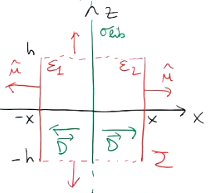
\includegraphics[width=0.3\linewidth]{lastra_piana_dielettrico}
\caption{Lastra piana carica}
\end{figure}
I due semipiani avranno costanti dielettriche differenti $\varepsilon_1$ 
ed $\varepsilon_2$.
Si studia il campo utilizzando la legge di Gauss:
$$
\oiint_{\Sigma} \vec{D}\cdot\hat{n}dS = Q_{lib}
$$
In questo caso si prende un parallelepipedo parallelo alle facce. La 
simmetria della distribuzione rispetto agli assi $y$ e $z$ fanno sì
che $\vec{D} = D_x(x)\vec{e}_x$ (in seguito $D_x$ sarà semplicemente $D$).

Applicando la legge di Gauss alla superficie $\Sigma$ si evince subito
che le superfici ortogonali ad $x$ non contribuiscono al flusso.
$$
\frac{\oiint_\Sigma \vec{D} \cdot \hat{n} dS }{hL}= -2\cancel{hL} D(-x) + 2\cancel{hL}D(x) = 
\sigma_{lib}\cancel{hL}
$$
Si evince la simmetria dispari del campo rispetto alla coordinata $x$ 
ossia $D(-x) = -D(x)$, sostituendo nella precedente si ottiene
$$
2D(x) = \sigma_{lib} \Rightarrow D(x) = \frac{\sigma_{lib}}{2}
$$
Il campo $\vec{D}$ è quindi pari in modulo e diretto in versi opposti
nei due semipiani. Per calcolare il campo $\vec{E}$ si potrà usare
la relazione costitutiva
$$
\vec{E} = \frac{\vec{D}}{\varepsilon}\Rightarrow
\begin{cases}
x > 0, & \vec{E}=\frac{\sigma_{lib}}{2\varepsilon_2} \vec{e}_x \\
x < 0, & \vec{E} = -\frac{\sigma_{lib}}{2\varepsilon_1} \vec{e}_x
\end{cases}\qquad
\begin{aligned}
\hat{n}\cdot(\vec{D}_2-\vec{D}_1) &= \sigma_{lib}\\
\hat{n}\cdot (\vec{E}_2-\vec{E}_1) &= \frac{\sigma_{lib}+\sigma_{pol}}{\varepsilon_0}
\end{aligned}
$$
Vale la continuità della componente normale di $\vec{D}$ ed $\vec{E}$.

\subsection{Condensatore piano con dielettrico}
Utilizzando il PSE, si prendono due strati indefiniti di carica $-\sigma_{lib}$ e $\sigma_{lib}$ mentre all'ascissa $x_0$ si trova un
cambio di dielettrico, come rappresentato in figura
\begin{figure}[H]
\centering
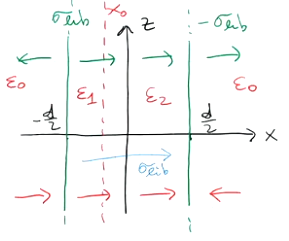
\includegraphics[width = 0.4\linewidth]{condensatore_dielettrici}
\caption{Lastre piane indefinite con dielettrici}
\end{figure}
Il campo $\vec{D}$ prodotto dall'armatura carica di sinistra sarà un campo uniforme
e diretto in verso uscente dalla lastra. Viceversa il campo prodotto
dalla lastra di destra sarà entrante nella lastra a causa del segno
opposto della carica.

La sovrapposizione degli effetti permette di calcolare il campo
totale eseguendo la somma dei due, all'esterno delle armature
il campo sarà quindi nullo mentre all'interno sarà di valore pari
a $\sigma_{lib}$
$$
\vec{D}(x) = \begin{cases}
\sigma_{lib} \vec{e}_x, & |x|<\frac{d}{2}\\
0 & \text{altrimenti}
\end{cases}
$$
È ora necessario calcolare il campo $\vec{E}$ e la capacità del 
condensatore, utilizzando i differenti valori di $\varepsilon$:
$$
\varepsilon = \begin{cases}
\varepsilon_0, & x< -\frac{d}{2}\\
\varepsilon_1, & -\frac{d}{2} < x < x_0 \\
\varepsilon_2, & x_0 < x < \frac{d}{2}\\
\varepsilon_0, & x>\frac{d}{2}
\end{cases}
$$
Sfruttando le relazioni costitutive si può ora calcolare
il campo $\vec{E}$
$$
E(x) = \begin{cases}
0, & x < -\frac{d}{2} \\
\frac{\sigma_{lib}}{\varepsilon_1}, & -\frac{d}{2} < x < x_0\\
\frac{\sigma_{lib}}{\varepsilon_2}, & x_0 < x < \frac{d}{2}\\
0, & x > \frac{d}{2}
\end{cases}
$$
Per calcolare la differenza di potenziale è sufficiente calcolare la 
differenza tra la funzione potenziale all'ascissa $-\frac{d}{2}$ e un 
punto $x$ generico
\begin{align*}
&V\left(-\frac{d}{2}\right) - V(x) = \int_{-\frac{d}{2}}^{x} \frac{\sigma_{lib}}{\varepsilon_1} d\xi = \frac{\sigma_{lib}}{\varepsilon_1}\left(x+\frac{d}{2}\right), -\frac{d}{2} < x < x_0 \Rightarrow V(x) = V^+ - \frac{\sigma_{lib}}{\varepsilon_1}\left(x + \frac{d}{2}\right)\\
&V(x_0 )- V(x) = \int_{x_0}^{x} \frac{\sigma_{lib}}{\varepsilon_2} d\xi = \frac{\sigma_{lib}}{\varepsilon_2} (x-x_0), x_0<x<\frac{d}{2}  \Rightarrow V(x) = V^+ - \frac{\sigma_{lib}}{\varepsilon_1}\left(x_0+\frac{d}{2}\right) - \frac{\sigma_{lib}}{\varepsilon_2}(x-x_0)
\end{align*}
Eseguendo quindi la differenza tra i potenziali sulle due armature si ottiene:
$$
V\left(-\frac{d}{2}\right) - V\left(\frac{d}{2}\right) = \cancel{V^+} - \left[ \cancel{V^+} -\frac{\sigma_{lib}}{\varepsilon_1}\left(x_0+\frac{d}{2}\right) - \frac{\sigma_{lib}}{\varepsilon_2} (x-x_0)\right] = \sigma_{lib} \left[\frac{1}{\varepsilon_1}\left(x_0+\frac{d}{2}\right) + \frac{1}{\varepsilon_2}\left(\frac{d}{2}-x_0\right)\right]
$$

La capacità sarà quindi 
$$
C = \frac{Q_{lib}}{V\left(-\frac{d}{2}\right) - V\left(\frac{d}{2}\right)} = 
\frac{\cancel{\sigma_{lib}}S}{\cancel{\sigma_{lib}} \left[ \frac{1}{\varepsilon_1}\left(x_0+\frac{d}{2}\right) + \frac{1}{\varepsilon_2}\left(\frac{d}{2}-x_0\right) \right] }
$$
Semplificando:
\begin{equation}
C = \frac{1}{ \frac{1}{\varepsilon_1S} \left(x_0 + \frac{d}{2} \right) + \frac{1}{\varepsilon_2S} \left( \frac{d}{2} - x_0 \right) } = \frac{1}{\frac{1}{C_1}+\frac{1}{C_2}}
\label{eq:condensatore_dielettrico}
\end{equation}
Nel condensatore vuoto la capacità era
$$
C_{\text{vuoto}} = \varepsilon_0\frac{S}{d}
$$
Si nota quindi che al denominatore della \ref{eq:condensatore_dielettrico} c'è la somma di due
reciproci di capacità $\frac{1}{C_1}$ e $\frac{1}{C_2}$ dove $C_1$ e $C_2$ sono appunto
$$
C_1 = \varepsilon_1 \frac{S}{x_0 + \frac{d}{2}} \qquad C_2 = \varepsilon_2 \frac{S}{\frac{d}{2}-x_0}
$$
Si vede quindi che la formula ottenuta è identica a quella di due condensatori in serie,
il primo di spessore $x_0 + \frac{d}{2}$ e il secondo $\frac{d}{2}-x_0$ adiacenti sulla faccia
$x_0$ e ciascuno con la propria costante dielettrica.

Lo stesso risultato si sarebbe potuto ottenere utilizzando il \textit{principio di metallizzazione delle 
superfici equipotenziali}.

Siccome la funzione potenziale è anch'essa funzione della sola coordinata $x$,  le superfici 
equipotenziali sono del tipo $x=a$, qualunque piano perpendicolare all'asse $x$ è una superficie
equipotenziale.

In virtù dell'unicità dei problemi dei valori al contorno dell'equazione di Laplace (o Poisson)
si può sostituire alla superficie di interfaccia tra i dielettrici, nel punto $x_0$ un conduttore
metallico stratiforme.
Fatto ciò è evidente vedere i due condensatori, la superficie metallica funge proprio
da armatura per entrambi i condensatori, disposti in serie.
\newpage
\subsection{Richiami su condensatori in serie e in parallelo}
\paragraph{Sistema serie}
\begin{figure}[H]
\centering
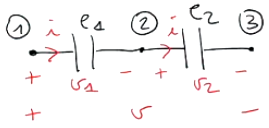
\includegraphics[width = 0.3\linewidth]{condensatori_serie}
\end{figure}
Presi due condensatori $C_1$ e $C_2$ disposti in serie, saranno attraversati dalla stessa corrente
$i$ e nel circuito saranno presenti tre potenziali sui nodi (1), (2) e (3).

Le equazioni caratteristiche sono:
\begin{align*}
&i = C_1 \frac{dv_1}{dt}\\
&v_1(t_0) = V_{10}\\
&i = C_2 \frac{dv_2}{dt} \\
&v_2(t_0) = V_{20}
\end{align*}
\begin{align}
v(t) = v_1(t) + v_2(t)
\label{eq:relazione_serie}
\end{align}
Integrando la prima e la terza relazione tra $t_0$ e $t$ si ottiene
\begin{align*}
&\int_{t_0}^t i(\tau) d\tau = C_1 \left[v_1(t) - V_{10}\right] \\
&\int_{t_0}^t i(\tau)d\tau = C_2 \left[v_2(t) - V_{20}\right]
\end{align*}
e sottraendo membro a membro
$$
C_1 \left[v_1(t) -V_{10}\right] = C_2\left[v_2(t) - V_{20}\right]
$$
Ricaviamo $v_2$ dalla precedente
$$
v_2(t) = V_{20} + \frac{C_1}{C_2} \left[v_1(t) - V_{10} \right]
$$
Utilizzando la relazione \ref{eq:relazione_serie} e sostituendo $v_2$ si ottiene
$$
v_1(t) = v(t) - V_{20} - \frac{C_1}{C_2} \left[v_1(t) - V_{10}\right]
$$
$$
v_1(t)\left(1+\frac{C_1}{C_2}\right) = v(t) - V_{20} + V_{10}\frac{C_1}{C_2}
$$
$$
v_1(t) = \frac{C_2}{C_1+C_2} v(t) + \frac{C_2}{C_1+C_2}\left[\frac{C_1}{C_2}V_{10}-V_{20}\right]
$$
$$
v_2(t) = \frac{C_1}{C_1+C_2} v(t) + \frac{C_1}{C_1+C_2}\left[\frac{C_2}{C_1}V_{20}-V_{10}\right]
$$
Sostituendo l'equazione di $v_1(t)$ nella caratteristica $i = C_1\frac{dv_1}{dt}$ si 
ottiene 
$$
i = \frac{C_1C_2}{C_1+C_2}\frac{dv}{dt}
$$
dato che il secondo termine di $v_1(t)$ è costante e la sua derivata è nulla. Il 
coefficiente ottenuto è proprio la capacità equivalente della serie.

\paragraph{Condensatori in parallelo}
\begin{figure}[H]
\centering
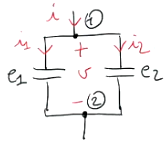
\includegraphics[width = 0.3\linewidth]{condensatori_parallelo}
\end{figure}

I due condensatori sono sottoposti alla stessa tensione $v$ ma attraversati da due
differenti correnti.
\begin{align*}
&i_1 = C_1 \frac{dv}{dt} \\
& i _2 = C_2 \frac{dv}{dt} \\
& v(t_0) = V_0
\end{align*}
In questo caso, a differenza del precedente si ha una sola grandezza di stato.
Sfruttando la legge di Kirchhoff delle correnti al nodo (1) si ottiene
$$
i = i_1 + i_2 = (C_1+C_2) \frac{dv}{dt}
$$
quindi
$$
\frac{dv}{dt} = \frac{i}{C_{eq}} \Rightarrow \begin{cases}
i_1 = \frac{C_1}{C_{eq}}i = \frac{C_1}{C_1+C_2}i\\
i_2 = \frac{C_2}{C_{eq}}i = \frac{C_2}{C_1 + C_2}i
\end{cases}
$$

\subsection{BVP per condensatore a due dielettrici}
\begin{figure}[H]
\centering
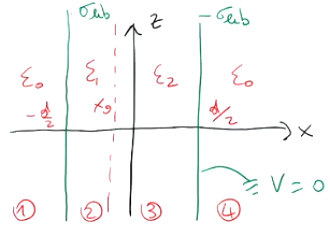
\includegraphics[width = 0.3\linewidth]{condensatore_dielettrici_2}
\end{figure}
Rappresentiamo graficamente il condensatore, applichiamo le equazioni
di Laplace alle diverse regioni
\begin{align*}
\nabla^2 V_1 = 0 \qquad & x< -\frac{d}{2} & V_1(x) = Ax + B\\
\nabla^2 V_2 = 0 \qquad & -\frac{d}{2} < x < x_0 & V_2(x) = Cx + D\\
\nabla^2 V_3 = 0 \qquad & x_0 < x < \frac{d}{2} & V_3(x) = Ex + F \\
\nabla^2 V_4 = 0 \qquad & x > \frac{d}{2} & V_4(x) = Gx + H
\end{align*}
Ricordando che in un problema monodimensionale
$$
\nabla^2 V = \frac{d^2 V}{dx^2} = 0 \Rightarrow V(x) = k_1x + k_2
$$
Si impostano due costanti per ogni regione, per un totale di 8
determinabili mediante le condizioni al contorno e di raccordo.

Le condizioni sono:
\begin{align*}
1) \qquad &V_1\left(-\frac{d}{2}\right) = V_2\left(-\frac{d}{2}\right)\\
2) \qquad &V_2\left(x_0\right) = V_3\left(x_0\right)\\
3) \qquad &V_3\left(\frac{d}{2}\right) = V_4\left(\frac{d}{2}\right)\\
4) \qquad  &
-\varepsilon_1 \left.\frac{\partial V_2}{\partial x}\right|_{-\frac{d}{2}} +
\varepsilon_0 \left.\frac{\partial V_1}{\partial x}\right|_{-\frac{d}{2}} = 
\sigma_{lib}\\
5) \qquad &-\varepsilon_2 \left.\frac{\partial V_3}{\partial x}\right|_{x_0} +
\varepsilon_1 \left.\frac{\partial V_2}{\partial x}\right|_{x_0} = 
0\\
6) \qquad &-\varepsilon_0 \left.\frac{\partial V_4}{\partial x}\right|_{\frac{d}{2}} +
\varepsilon_2 \left.\frac{\partial V_3}{\partial x}\right|_{\frac{d}{2}} = 
-\sigma_{lib}\\
7) \qquad &V_3\left(\frac{d}{2}\right) = 0 \qquad \text{pot. di riferimento}\\
8-9) \qquad& -\frac{\partial V_1}{\partial x} ,\ -\frac{\partial V_4}{\partial x} = 0\ \ |x| > \frac{d}{2}\ \ \text{campo esterno nullo}
\end{align*}
Il potenziale di riferimento è necessario dato che essendo le superfici cariche 
infinite, non si ha un potenziale normale all'infinito, questo
viola il teorema di unicità della soluzione rendendo necessario il riferimento.
Non conta il valore di riferimento assegnato dato che la grandezza di interesse
è il campo elettrico, ossia il gradiente del potenziale che non dipende
dal suo riferimento.

L'ultima condizione (8-9) deriva dall'estensione all'infinito dei modelli al 
finito che prevedono un campo elettrico concentrato al centro. Anche i modelli
all'infinito devono rispettare quindi la normalità all'infinito, ossia il
campo deve essere nullo al di fuori delle armature.

Riscrivendo le equazioni con le costanti incognite si ottiene:
\begin{align*}
1)   \qquad & A\left(-\frac{d}{2}\right) + B = C\left(-\frac{d}{2}\right) + D \\
2)   \qquad & Cx_0 + D = Ex_0 + F \\
3)   \qquad &E\frac{d}{2} + F = G \frac{d}{2} + H \\
4)   \qquad &- \varepsilon_1 C + \varepsilon_0 A = \sigma_{lib} \\
5)   \qquad &- \varepsilon_2 E + \varepsilon_1 C = 0 \\
6)   \qquad &-\varepsilon_0G = \varepsilon_2 E = -\sigma_{lib} \\
7)   \qquad & E\frac{d}{2} + F = 0 \\
8-9) \qquad & A = G = 0
\end{align*}

Ci sono quindi 9 equazioni in 8 incognite e si può vedere che il sistema 
ha rango 8.
Si può porre il sistema lineare con notazione matriciale nel seguente modo:
\begin{align*}
\underline{\underline{A}}\ \underline{x} &= \underline{b}\\
\underline{x} &= \left(A,B,C,D,E,F,G\right)^T \\
\underline{b} &= \left(0,0,0,\sigma_{lib},0,-\sigma_{lib},0,0\right)^T 
\end{align*}
Mentre la matrice $\underline{\underline{A}}$ si deduce dall'analisi delle 
equazioni. 
\newpage
Di seguito è riportato un esempio per risolvere numericamente
il problema.
\begin{lstlisting}[style=Matlab-editor,language = Matlab]
syms d Vp x0 ep0 ep1 ep2 slib x real

A = [ -d/2   1   d/2   -1   0   0   0   0;
        0    0    x0    1  -x0 -1   0   0;
        0    0    0     0  d/2  1 -d/2 -1;
       ep0   0  -ep1    0   0   0   0   0;
        0    0   ep1    0 -ep2  0   0   0;
        0    0    0     0  ep2  0 -ep0  0;
        0    0    0     0  d/2  1   0   0;
        1    0    0     0   0   0   0   0;
        0    0    0     0   0   0   1   0];

b=[0;0;0;slib;0;-slib;0;0;0];

%K Vettore delle costanti incognite "equivale" a inv(A)*b anche se e' preferibile questa forma
K=A\b;

%Si ricavano le diverse tensioni
V1=K(1)*x+K(2);
V2=K(3)*x+K(4);
V3=K(5)*x+K(6);
V4=K(7)*x+K(8);

%Vettore delle tensioni risolte
V=[V1;V2;V3;V4] 

%derivata di V rispetto a x
E=-diff(V,x) 

%Componenti del campo D ottenute con le differenti epsilon
D=diag([ep0,ep1,ep2,ep0])*E 
\end{lstlisting}
La matrice $\underline{\underline{A}}\ [9\times 8]$ rappresenta quindi i coefficienti delle
costanti delle equazioni che moltiplicati per il vettore delle incognite
forniscono il vettore dei termini noti $\underline{b}$.
Analizzando i risultati si vede che questi sono coerenti con quelli ottenuti
analiticamente dall'analisi precedente.
È possibile visualizzare un laboratorio virtuale di campi elettrostatici al seguente link:
\href{http://falstad.com/vector3de/vector3de.html?f=InverseSquaredRadialDipole&d=equip&sl=y&p=1&a1=29&rx=92&ry=0&rz=-1&zm=1.2}{www.falstad.com/vector3de}, sullo stesso sito è possibile visualizzare diversi applet riguardanti ambiti
diversi della fisica.

\subsection{Formulazione debole dell'equazione di Poisson (FEM)}
\begin{equation*}
\begin{cases}
\nabla^2u = f & \text{in }\Omega\\
\left. u \right|_{\partial\Omega} = g
\end{cases}
\end{equation*}
$$
u \in C^2(\Omega),\ f \in C^0(\Omega),\ g\in C^0(\partial\Omega)
$$
In queste condizione la soluzione esiste ed è unica.
La soluzione di classe $C^2$ viene chiamata \textbf{forte} in termini di regolarità
ossia è molto regolare.

Normalmente quando si applica il \textit{metodo degli elementi finiti} (FEM) 
i requisiti sulla funzione incognita $u$ sono meno stringenti e si
parla di soluzione \textbf{debole}.

Si considera uno spazio di funzioni \textit{test} chiamate funzioni
``peso''  $p \in C^1_0\ : \ p(\partial\Omega) = 0$

Moltiplicando ambi i membri dell'equazione di Poisson e integrando si ottiene:
$$
\iiint_\Omega p\nabla^2 u dV = \iiint_\Omega p f dV
$$
Ricordando l'identità vettoriale $p\nabla^2 u = \nabla\cdot \left(p\nabla u\right) - \nabla p\cdot \nabla u $

Sostituendo si ottiene:
$$
\iiint_\Omega p f dV = \iiint_{\Omega} \left(\nabla\cdot\left(p\nabla u\right)-\nabla p\cdot\nabla u\right)dV
$$
Applicando il teorema della divergenza
$$
\iiint_\Omega p f dV = \cancel{\iint_{\partial\Omega} p \frac{\partial u}{\partial n}dS} - \iiint_\Omega \nabla p\cdot\nabla u\ dV
$$
Siccome la funzione $p$ test scelta è nulla sulla frontiera, il primo termine della differenza si azzera:
$$
\iiint_\Omega p f dV = \iiint_\Omega -\nabla p\cdot\nabla u\ dV\ \ \forall\ p\in C^1_0(\Omega)
$$
Quella appena ottenuta è proprio la formazione debole del BVP iniziale.

Introducendo $u_\partial : u_\partial = g\ \text{su } \partial\Omega\ : \ u = \hat{u} + u_\partial$ ossia prolungando
la funzione $g$ all'interno del dominio, si può ricavare la funzione $\hat{u}$ differenza tra le due.

Si vede dunque che $\hat{u}$ è soluzione di un BVP per la stessa equazioni con condizioni di
Dirichlet omogenee, ossia $\hat{u} = 0\ \text{su } \partial\Omega$.

Sostituendo la funzione $u$ estesa nell'integrale precedente si ottiene
$$
-\iiint_\Omega \nabla p \cdot \nabla\hat{u}\  dV = \iiint_\Omega p f dV +
\iiint_\Omega \nabla p \cdot \nabla u_\partial\ dV\ \forall\ p\in C^1_0(\Omega)
$$
I due integrali a destra dell'uguaglianza sono termini noti, l'espressione rappresenta
una famiglia di equazioni integrali nell'incognita $\hat{u}$ al variare
di $p$ nello spazio delle funzioni test.

\newpage
\subparagraph{\href{https://it.wikipedia.org/wiki/Metodo_di_Gal\%C3\%ABrkin}{Metodo di Galërkin}}
Consiste nel ricercare una soluzione espressa mediante la base di uno spazio
a dimensione finita chiamato ad esempio $W^0_M$ dove $M$ è il numero di
gradi di libertà da utilizzare ossia quanto più accurata sarà la soluzione,
se al limite $M$ fosse infinito avrei una soluzione identica al continuo.

Supposta una base $\hat{u}_M$ per questo spazio di funzioni che si 
annullano sulla frontiera a dimensione finita $M$
$$
\hat{u}_M = \sum_{k = 1}^{M} a_k w_k \ \ \text{ con } w_k \text{ funzioni di base di } W_m^0
$$
Sostituendo nell'integrale del paragrafo precedente
$$
-\iiint_\Omega \nabla w_h \cdot \nabla \left(\sum_{k=1}^{M} a_k w_k \right) dV = 
\iiint_\Omega w_h f dV + \iiint_\Omega \nabla w_h \cdot \nabla u_\partial\ dV\ \ h=1,...,M
$$
I coefficienti $a_k$ per linearità si possono tirar fuori dall'integrale
$$
-\sum_{k=1}^M \left(\iiint_\Omega \nabla w_h \cdot \nabla w_k\ dV \right) a_k = 
\iiint_\Omega w_h f dV + \iiint_\Omega \nabla w_h \cdot \nabla u_\partial\ dV
$$
Svolgendo l'integrale tra parentesi e risolvendo gli integrali a destra
$$
-\sum_{k=1}^M L_{hk} a_k = b_h\ \ h=1,...,M
$$
L'equazione ottenuta si trasforma in un sistema lineare algebrico del tipo:
$$
\underline{L}_M \cdot \underline{a}_M = \underline{b}_M
$$
Se si ipotizza una forma per le funzioni test è possibile calcolare i coefficienti
$L_{hk}$ e risolvere il sistema.

\newpage
\subparagraph{Metodo degli elementi finiti}
\begin{figure}[H]
\centering
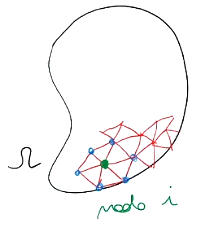
\includegraphics[width = 0.2\linewidth]{esempio_dominio_mesh}
\caption{Esempio dominio con MESH}
\end{figure}
Consiste nel partizionare ad esempio con strutture triangolari o tetraediche un dominio.
Si definisce su ogni nodo $i$ della griglia una funzione test $w_i$

$$
w_i(\underline{x}) = \begin{cases}
1 & \text{se } \underline{x} = \underline{x}_i\\
0 & \text{se } \underline{x} \neq \underline{x}_i\\
&\text{lineare intorno al nodo }\underline{x}_i
\end{cases}
$$
Vengono definite funzioni ``a tenda'' data la loro somiglianza ad una tenda canadese.
È possibile calcolare tutti i coefficienti una volta ottenuta la \textit{MESH} del
dominio, ossia la sua completa triangolazione.
Una volta nota è possibile assegnare facilmente le funzioni tenda e calcolare i
coefficienti $L_{hk}$ e $b_h$ note le funzioni $f$ e $g$.
All'aumentare di $M$ ossia del numero di nodi migliora la descrizione
della geometria.

In MATLAB è possibile usare la \textit{Partial Differential Equation Toolbox}, per 
gli amici ``pdetool'' per accedere ad un'interfaccia grafica che permette
di impostare una geometria e risolvere questo genere di problemi.


\subparagraph{Calcolo della capacità di un condensatore con MATLAB}
Si ricorda il modello dell'elettrostatica
$$
\begin{cases}
\nabla \times \vec{E} = 0 &\text{in } \Omega \Rightarrow \vec{E} = -\nabla u\\
\nabla\cdot\vec{D} = 0 &\text{in }\Omega\text{ non ci sono cariche libere}\\
\vec{D} = \varepsilon\vec{E} &\text{in } \Omega\text{ materiale omogeneo ed isotropo}
\end{cases}
$$
Il modello si trasforma in questo caso nel problema dei valori al contorno
per l'equazione di Laplace con condizioni di Dirichlet sugli elettrodi
e condizione alla Neumann su una frontiera abbastanza lontana da approssimare
l'infinito.
$$
\begin{cases}
\nabla^2 u = 0 & \text{in } \Omega\\
\left.u\right|_{l_1} = V_1\\
\left.u\right|_{l_2} = 0\\
\left.\frac{\partial u}{\partial n}\right|_{\partial\Omega e} = 0
\end{cases}
$$
Le funzioni ``tenda'' solitamente utilizzate nei metodi agli elementi finiti
sono lineari a tratti, ad esempio la funzione $w_i$ vale $1$ nel nodo
in cui è valutata e decresce linearmente a $0$ nei nodi adiacenti.
Il grado del polinomio della funzione test può essere incrementato ma
si incrementano anche i problemi analitici dovuti al rispetto
delle condizioni al contorno e di raccordo, per questo motivo sono solitamente
utilizzati polinomi di grado 1.
\begin{figure}[H]
\centering
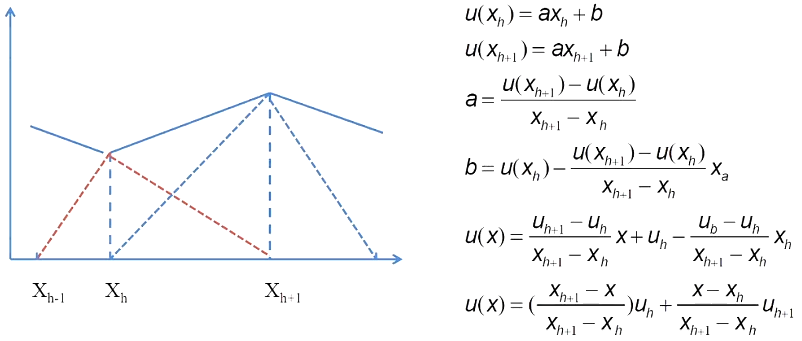
\includegraphics[width=0.7\linewidth]{funzione_tenda}
\caption{Espressione analitica funzione tenda di grado 1}
\end{figure}
Per ricostruire la funzione si esegue una combinazione lineare delle
funzioni tenda nei vari punti.

Per domini bidimensionali è ancora possibile eseguire una discretizzazione
in elementi triangolari, con funzioni lineari in due variabili,
la matrice dei coefficienti risultante è simmetrica e semidefinita
positiva, inoltre è una matrice sparsa, ossia i coefficienti pari a zero sono 
molto maggiori rispetto a quelli diversi da zero, ciò è vantaggioso
durante il calcolo del prodotto matriciale, necessario alla risoluzione
del problema.
\begin{figure}[H]
\centering
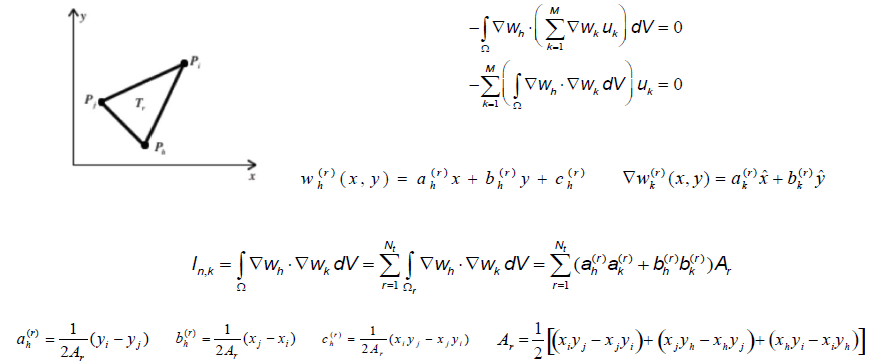
\includegraphics[width=0.7\linewidth]{tenda_bidimensionale}
\caption{Espressione funzione tenda bidimensionale}
\end{figure}

Per impostare un problema con il \textit{pdetool} è necessario
seguire i seguenti passaggi:
\begin{enumerate}
\item Definizione del problema fisico e del suo modello matematico
\item Definizione della geometria con ausilio di CAD
\item Imposizione delle condizioni al contorno
\item Discretizzazione del dominio (\textit{meshing}), l'errore aumenta
all'aumentare dell'irregolarità dei triangoli
\item Si assegnano le matrici dei termini noti e si risolve il sistema lineare
\end{enumerate}

\subparagraph{Dominio bucato con pdetool}
Si riassumono brevemente gli step da eseguire per studiare un dominio quadrato
al quale vengono sottratte due circonferenze ad esso interne.

Si piazzano e si disegnano il rettangolo e le circonferenze, è poi
fondamentale impostare la ``formula'' del dominio, ossia la pseudo-equazione
che descrive logicamente il dominio da analizzare; in questo caso si sta
trattando un quadrato bucato, chiamato $R1$ il rettangolo e $E1$ ed $E2$ 
le due circonferenze, la ``formula'' sarà quindi $R1-E1-E2$.

Definita la geometria vanno assegnate le condizioni al contorno mediante il menù ``Boundary'' e impostare le condizioni di Dirichlet per specificare
ad esempio il potenziale di quel lato a 0 oppure 1 e -1 sugli elettrodi
sferici.

In ``PDE'' è possibile specificare la costante dielettrica relativa del
dominio e la densità di carica libera al suo interno, questi due valori
nell'esempio sono stati posti rispettivamente a 1 e 0.

Si può ora procedere al meshing del dominio eseguendo successivamente
un numero appropriato di ``raffinamenti'' ossia di riduzioni delle
dimensioni degli elementi.

Premendo sul pulsante '$=$' è possibile risolvere il problema, il risolutore
mostrerà di default il potenziale con una scala di colori. Cambiando le 
impostazioni è possibile rappresentare diverse grandezze, aggiungere 
isolinee del potenziale o linee di forza del campo.
\newpage
Si ottiene un risultato simile:
\begin{figure}[H]
\centering
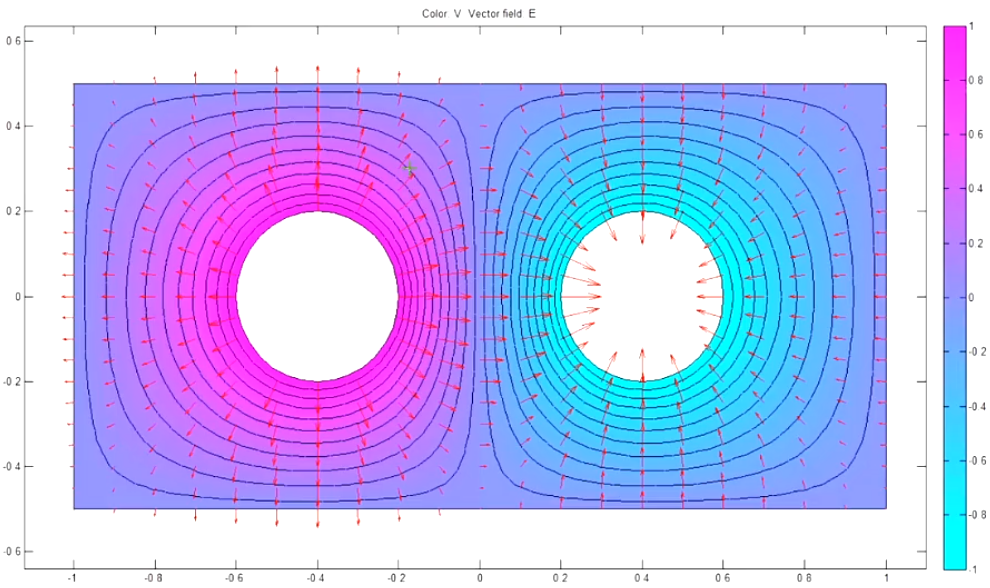
\includegraphics[width=0.8\linewidth]{potenziale_due_conduttori_FEM}
\caption{Potenziale e vettori forza prodotti da due conduttori carichi}
\end{figure}

È possibile utilizzare il \textit{pdetool} mediante la riga di comando
o uno script MATLAB
\begin{lstlisting}[style=Matlab-editor,language = Matlab]
%Definizione del rettangolo
pderect([xmin xmax ymin ymax],'R1');
%Definizione della circonferenza
pdecirc(xc,yc,r,'E1');
%Impostazione della set formula
set(findobj(get(pde_fig,'Children'),'Tag','PDEEval'),'String','R1-E1');
%Esportazione della geometria
bl=get(findobj(get(pde_fig,'Children'),'flat','Tag','PDEBoundMenu'),'UserData');
%Impostazioned elle boundary
%Neumann
pdesetbd(5,'neu',1,'0','0');
%Dirichlet, V e' la variabile stringa del potenziale num2str(10)
pdesetbd(4,'dir',1,'1',V);
%Generazione della MESH
[p1,e1,t1]=initmesh(dl,'Hmax',0.01,'init','off');
%rifinitura
[p,e,t]=refinemesh(dl,p1,e1,t1,'regular');
%Plot della MESH
pdeplot(p,e,t);
\end{lstlisting}
I numeri indicati nel comando ``pdesetbd'' si possono ricavare dal menù
Boundary $>$ Show Edge Labels, corrispondono all'identificativo del lato
del dominio.

La matrice $p$ contiene le coordinate dei nodi della mesh.

La matrice $e$
contiene i nodi del contorno, le prime due righe contengono gli indici
dei nodi iniziali e finali dei segmenti del contorno, la terza e la quarta
contengono i valori iniziali e finali del parametro, la quinta contiene
il numero identificativo del segmento di frontiera, la sesta e la settima
contengono i numeri dei sottodomini a destra e sinistra del segmento.

La matrice $t$ o matrice dei triangoli fornisce la relazione di appartenenza tra 
nodi e triangoli, la n-esima colonna coincide con l'n-esimo triangolo e contiene
la terna antioraria degli indici dei nodi dei suoi vertici.

Verificata la coerenza della mesh è possibile assemblare il problema e risolverlo
\begin{lstlisting}[style=Matlab-editor,language = Matlab]
u=assempde(bl,p,e,t,c,a,f);
\end{lstlisting}

\subsection{Capacità di un condensatore con FEM}
Si definiscono le equazioni del problema
$$
\begin{cases}
\nabla^2u = 0\\
\left. u\right|_{l_1} = 10\\
\left. u\right|_{l_2} = 0\\
\left.\frac{\partial u}{\partial n}\right|_{\text{inf}} = 0
\end{cases}
\Rightarrow
\begin{cases}
\frac{1}{\rho}\left(\frac{\partial}{\partial \rho}\left(\rho\frac{\partial}{\partial\rho}u\right)+
\frac{\partial}{\partial z}\left(\rho\frac{\partial}{\partial z}u\right)\right)=0\\
\left. u\right|_{l_1} = 10\\
\left. u\right|_{l_2} = 0 \\
\rho\left.\frac{\partial u}{\partial n}\right|_{\text{inf}} = 0
\end{cases}
$$
\begin{figure}[H]
\centering
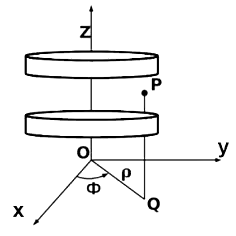
\includegraphics[width = 0.25\linewidth]{geom_condensatore_FEM}
\caption{Geometria condensatore con armature cilindriche}
\end{figure}
Il sistema è simmetrico rispetto all'asse $z$ e il problema
viene formulato mediante coordinate polari.
All'aumentare del raggio dei dischi, il condensatore si comporta come
un condensatore piano indefinito, trascurando gli effetti di bordo,
allontanandosi dal dispositivo invece si vede come il campo prodotto
all'esterno sia simile a quello di un dipolo.
\newpage
Sfruttando la simmetria della struttura è possibile analizzare il problema
studiandone metà, questo permette di ridurre i costi computazionali data la
dimensione ridotta della mesh.
\begin{lstlisting}[style=Matlab-editor,language = Matlab]
%definizione coordinate
xmin=0;
xmax=0.1;
ymin=-0.1;
ymax=0.1;
%Spessore dielettrico
dh=7.5e-4;
%Costante dielettrica relativa
epsr=2.9;
%Definizione rettangoli rappresentanti le armature
pderect([xmin xmax dh/2 ymax],'R1');
pderect([xmin xmax -dh/2 ymin],'R2');
%Dominio esterno
pderect([1.5*xmin 1.5*xmax 5*ymin 5*ymax],'R3');
%Impostazione regola dominio (set string)
set(findobj(get(pde_fig,'Children'),'Tag','PDEEval'),'String','R3-R2-R1');
%Esportazione dominio
dl=get(findobj(get(pde_fig,'Children'),'flat','Tag','PDEBoundMenu'),'UserData');
\end{lstlisting}
Si impongono le condizioni di Neumann sul dominio esterno, mentre quelle di 
Dirichlet sulle due armature, impostando due potenziali arbitrari.

Si esegue il meshing
\begin{lstlisting}[style=Matlab-editor,language = Matlab]
[p1,e1,t1]=initmesh(dl,'Hmax',0.1,'init','off');
[p,e,t]=refinemesh(dl,p1,e1,t1,'regular');
%Coordinata rho del baricentro dei triangoli
x=pdeinterp(p,t,p(1,:)');
%Calcolo soluzione
u=assempde(dl,p,e,t,x,'0','0');
\end{lstlisting}
Si vede che la mesh è molto disuniforme, molto fitta tra le armature e meno
all'esterno e verso i bordi. Per calcolare la capacità si valuta l'energia
immagazzinata, ricordando che in questo caso $v=Ed$
$$
w_e(t) = \frac{1}{2}Cv(t)^2 = \frac{1}{2}\varepsilon\frac{S}{d}v(t)^2 = 
\frac{1}{2}\varepsilon SdE^2
$$
Conoscendo il campo elettrico nel volume tra le due armature
$$
\frac{1}{2}Cv^2 = \iiint_{\mathbb{R}^3}\varepsilon \frac{E^2}{2}dV
$$
Conoscendo il secondo termine dalle simulazioni e la tensione imposta, si ricava
facilmente la capacità.
$$
\text{Energia } = \frac{1}{2}\varepsilon\cdot\int_0^{2\pi} d\theta 
\int_{zmin}^{zmax}\int_0^{\rho max} \left|E(r,z)\right|^2\cdot \rho\ d\rho\ dz =
\frac{1}{2}C\Delta V^2
$$
$$
C = \frac{\varepsilon\cdot \int_0^{2\pi} d\theta 
\int_{zmin}^{zmax}\int_0^{\rho max} \left|E(r,z)\right|^2\cdot \rho\ d\rho\ dz}{\Delta V^2}
$$
Risolvendo il calcolo su MATLAB
\begin{lstlisting}[style=Matlab-editor,language = Matlab]
[UX,UY] = pdegrad(p,t,u);
%Numero dei triangoli
Nt = size(t,2);
%area di ogni triangolo
area = abs(pdetrg(p,t));    

Energia = 0;
for n = 1:Nt     
    E2 = (UX(n)^2+UY(n)^2);  %norm(E)^2
    Energia = Energia+0.5*eps0*E2*area(n)*1;
end

%Capacita' teorica e numerica
Cteor = eps0*height*1/dist
Cnum = 2*Energia/(v1-v2)

%Errore relativo
e_rel = (Cnum-Cteor)/Cteor
\end{lstlisting}
È possibile visualizzare analoghe simulazioni negli appunti in pdf
su questa lezione.

\subparagraph{Risolutore circuiti simbolico}
Al seguente link \href{http://143.225.92.177:54323/}{tinyurl.com/ss2lcsmda}
è possibile vedere un solutore di circuiti simbolico che sfrutta la 
trasformata di Laplace e fornisce la soluzione nel dominio del tempo.
Il seguente circuito d'esempio deve essere trasformato in \textit{netlist} per 
essere risolto con il software.
\begin{figure}[H]
\centering
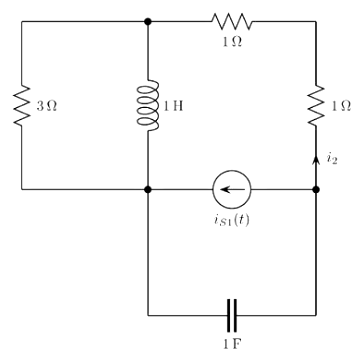
\includegraphics[width = 0.3\linewidth]{circuito_risolutore_simbolico}
\caption{Esempio circuito da risolvere con il risolutore}
\end{figure}
La netlist è una tabella contenente in ordine
il tipo di bipolo, il nodo iniziale e il
nodo finale, il valore della sua grandezza caratteristica.
La netlist dell'esempio si può generare in questo modo:

\begin{lstlisting}[frame = single]
J 0 1 delta(t)
C 1 0 1
L 1 2 1
R1 1 2 3
R2 2 3 1
ZO 0 3 1
\end{lstlisting}
Selezionando la voce ``Laplace pre/post processing'' è possibile ottenere
la soluzione calcolata mediante la trasformata di Laplace.
Si ottengono tutte le funzioni di trasferimento delle grandezze caratteristiche.
È possibile calcolare l'antitrasformata su ``Wolfram Alpha'' seguendo
i link appropriati e confrontarli con i risultati nel dominio del tempo
forniti sulla stessa pagina o con MATLAB mediante il seguente codice:
\begin{lstlisting}[style=Matlab-editor,language = Matlab]
syms s;
H = - (s+3)/(5*s^2+7*s+3);
ilaplace(H)
pretty(ans)
\end{lstlisting}




\section{Esercizio}
Determinare 
\begin{enumerate}
\item Equazioni di stato
\item Risposta impulsiva
\begin{enumerate}
\item[2.a] Con il metodo delle condizioni iniziali con generatore impulsivo
\item[2.b] Con la risposta al gradino
\end{enumerate}
\item Funzione di trasferimento (L-trasformata e antitrasformata)
\end{enumerate}
\begin{figure}[H]
\centering
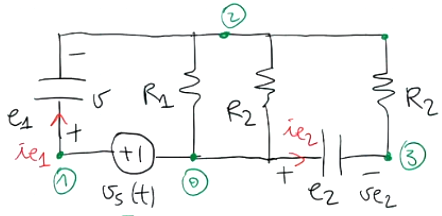
\includegraphics[width = 0.4\linewidth]{circuito_esercizio_1}
\end{figure}
$$
R_1 = \SI{2}{\ohm}\ \ R_2 = \SI{3}{\ohm}\ \ C_1 = \SI{3}{\farad}\ \ C_2 = \SI{1}{\farad}
$$
Per determinare le equazioni di stato si sostituisce il circuito con il circuito
resistivo associato, sostituendo ad ogni condensatore un generatore di tensione
equivalente e calcolando in seguito le correnti $i_{C_1}$ e $i_{C_2}$.
Sostituiti i condensatori si calcolano le correnti con il PSE.

Il primo circuito chiamato $C'$ ha solo la tensione $v_{C_1}$ diversa da zero
mentre gli altri generatori sono spenti (cortocircuiti), il circuito $C''$ ha il generatore $v_{C_2}$ attivo, il circuito $C'''$ ha il generatore $v_s$ attivo.

$$
\begin{aligned}
C' & \\
R_{eq} &= (R_1//R_2)//R_2\\
i_{C_1'} &= - \frac{V_{C_1}}{R_{eq}} \\
i_{C_2'} &= \frac{V_{C_1}}{R_2}
\end{aligned}
\qquad
\begin{aligned}
C'' & \\
i_{C_1'} &= \frac{V_{C_2}}{R_2}\\
i_{C_2'} &= -\frac{V_{C_2}}{R_2}
\end{aligned}
\qquad
\begin{aligned}
C''' & \\
i_{C_1'''} &= \frac{V_s}{R_{eq}} \\
i_{C_2'''} &= -\frac{V_s}{R_2}
\end{aligned}
$$
Si può ora applicare il principio di sovrapposizione degli effetti
sommando i vari contributi
$$
\begin{aligned}
i_{C_1} & = -\frac{V_{C_1}}{R_{eq}} + \frac{V_{C_2}}{R_2} + \frac{V_s}{R_{eq}} =
C_1\frac{dv_{C_1}}{dt}\\
i_{C_2} & = -\frac{V_{C_1}}{R_2} - \frac{V_{C_2}}{R_2} - \frac{V_s}{R_2} =
C_2\frac{dv_{C_2}}{dt}
\end{aligned}
$$
\subparagraph{2.a) Risposta all'impulso con C.I.}
Si determina ora la risposta impulsiva con il metodo delle condizioni iniziali con 
generatore impulsivo.
Si sostituiscono ancora una volta i bipoli dinamici con corto circuiti o circuiti
aperti (nel caso in cui siano condensatori o induttori) e si impone il generatore
$V_s(t) = \delta(t)$ ricordando che $R_{eq}=\frac{6}{7}\si{\ohm}$
\begin{align*}
i_{C_1} &= \frac{\delta(t)}{R_{eq}} = \frac{7}{6}\delta(t)\\
i_{C_2} &= -\frac{\delta(t)}{R_2} = -\frac{1}{3}\delta(t)
\end{align*}

Sostituendo con la caratteristica del condensatore e integrando si ha
\begin{align*}
\left(V_{C_1}(0^-) = \SI{0}{\volt}\right)\ \ C_1V_{C_1}(0^+) &=\int_{0^-}^{0^+}C_1\frac{dV_{C_1}}{dt}dt = \int_{0^-}^{0^+}\frac{7}{6}\delta(t)dt = \frac{7}{6} \Rightarrow V_{C_1}(0^+) = \frac{7}{18}\si{\volt}\\
\left(V_{C_2}(0^-) = \SI{0}{\volt}\right)\ \ C_2V_{C_2}(0^+) & = \int_{0^-}^{0^+} C_2 \frac{dV_{C_2}}{dt}dt =
\int_{0^-}^{0^+} -\frac{1}{3}\delta(t) dt = -\frac{1}{3} \Rightarrow V_{C_2}(0^+) = -\frac{1}{3}\si{\volt}
\end{align*}
Determinate le condizioni iniziali si sa che la soluzione del circuito è proprio
l'evoluzione libera, con generatore spento a partire da queste condizioni iniziali.

Si vuole ricavare la $V_{C_1}$, si ricava quindi $V_{C_2}$ dalla prima equazione di stato in funzione della $V_{C_1}$ e la si sostituisce nella seconda.
$$
V_{C_2} = R_2 \left( \frac{V_{C_1}}{R_{eq}} + C_1\frac{dV_{C_1}}{dt} \right)
$$
$$
\frac{V_{C_1}}{R_2} - \frac{V_{C_1}}{R_{eq}} - C_1\frac{dV_{C_1}}{dt} - \cancel{\frac{V_s}{R_2}} = 
C_2\left(\frac{R_2}{R_{eq}}\frac{dV_{C_1}}{dt} + R_2C_1\frac{d^2V_{C_1}}{dt^2}\right)
$$
$$
C_2C_1R_2\frac{d^2V_{C_1}}{dt^2} + \left(\frac{C_2R_2}{R_{eq}}+C_1\right)\frac{dV_{C_1}}{dt} +
\left(\frac{1}{R_{eq}}-\frac{1}{R_2}\right)V_{C_1} = 0
$$
Per verificare la correttezza dei calcoli si nota che dimensionalmente tutti i termini 
hanno sono la stessa grandezza (in questo caso la corrente) e che il segno dei coefficienti
sia concorde affinché la grandezza in esame nel circuito dissipativo si smorzi nel tempo.

Per trovare le radici del polinomio caratteristico è utile rendere unitario il coefficiente del
termine di grado più elevato.
$$
\lambda^2 + \left(\frac{1}{R_{eq}C_1} + \frac{1}{R_2C_2}\right)\lambda + \left(\frac{1}{R_{eq}}-\frac{1}{R_2}\right)\frac{1}{C_2C_1R_2} = 0
$$
$$
\lambda^2+\frac{13}{18}\lambda + \frac{5}{54} = 0
$$
Si calcolano dunque le radici:
$$
\lambda_{1,2} = -\frac{13}{36} \pm \sqrt{\left(\frac{13}{36}\right)^2-\frac{5}{54}} = 
\begin{cases}
\lambda_1 = -0.556\\
\lambda_2 = -0.167
\end{cases}
$$
La soluzione sarà del tipo
$$
V_{C_1}(t) = K_1 e^{-0.556 t} + K_2 e^{-0.167 t}
$$
\newpage
Si ricavano le costanti $K_1$ e $K_2$ mediante le condizioni iniziali prima ricavate.

$$
\begin{aligned}
V_{C_1}(0^+) &= \frac{7}{18} = K_1 + K_2 \\
\frac{dV_{C_1}}{dt}(0^+) &= -0.188 = \lambda_1K_1 + \lambda_2K_2
\end{aligned}
\Rightarrow
\begin{cases}
K_2 = 0.0714\\
K_1 = 0.3175
\end{cases}
$$
Assemblando il risultato si ottiene:
$$
V_{C_1}(t) = h(t) = 0.3175e^{-0.556 t} + 0.0714 e ^{-0.617 t}, \ \ t\geq 0
$$

\subparagraph{2.b) Modo alternativo con risposta al gradino}
Ricordando che nei punti regolari o nel senso delle distribuzioni $h(t) = \frac{dg}{dt}$.
Il gradino è una soluzione a regime, quindi si può recuperare il risultato precedente
e aggiungere la soluzione di regime.
Si sostituiscono nel circuito i condensatori con circuiti aperti
\begin{figure}[H]
\centering
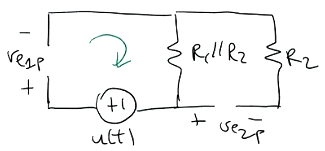
\includegraphics[width=0.6\linewidth]{circuito_esercizio_1_regime}
\end{figure}
$$
V_{C_{1p}} = u(t)
$$
$$
g(t) = K_1'e^{-0.556t} + K_2'e^{-0.167 t} + u(t)
$$
Ricordando che $u(t)=1,\ t>0$ si ricavano le nuove condizioni iniziali per determinare
i coefficienti $K_1'$ e $K_2'$
$$
\begin{aligned}
g(0^+) &= K_1' + K_2' + 1 = 0\\
\frac{dg}{dt}(0^+) &= \frac{1}{R_{eq}C_1} = \frac{7}{18}
\end{aligned}
\Rightarrow
\begin{aligned}
K_1' = -0.5704 \\
K_2' = -0.4296
\end{aligned}
$$
La risposta al gradino è dunque:
$$
g(t) = V_{C_1}(t) = -0.5704 e^{-0.556t} - 0.4296e^{-0.167t} + 1,\ t\geq 0
$$
$$
h(t) = \frac{dg}{dt} = 0.3175e^{-0.556t}+0.0714e^{-0.167 t},\ t\geq 0
$$
\newpage
\subparagraph{3) Funzione di trasferimento}
È utile per risolvere il problema nel dominio di Laplace.
Si trasforma il circuito in un circuito di ``impedenze operatoriali'',
si sostituisce ai condensatori un'impedenza $Z_c(s)$, il generatore viene sostituito
con la trasformata della $\delta(t)$ quindi un generatore di tensione di valore unitario.
\begin{figure}[H]
\centering
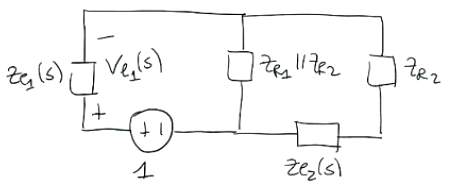
\includegraphics[width = 0.5\linewidth]{circuito_esercizio_1_Laplace}
\end{figure}
$$
Z_{C_1} = \frac{1}{C_1s}\ \ Z_{C_2} = \frac{1}{C_2s}\ \ Z_{R_1}//Z_{R_2} = \frac{6}{7}\ \ Z_{R_2} = 3
$$
Si deve quindi risolvere un circuito adinamico lineare con le normali tecniche di riduzione
sfruttando le equivalenze serie e parallelo.
$$
\begin{aligned}
Z_{eq}^{(1)} &= \frac{1}{C_2s} + R_2 = \frac{1}{s} + 3 \\
Z_{eq}^{(2)} & = \frac{Z_{eq}^{(1)}(Z_{R_1}//Z_{R_2})}{Z_{eq}^{(1)}+Z_{R_1}//Z_{R_2}} = 
\frac{\left(\frac{1}{s}+3\right)\frac{6}{7}}{\left(\frac{1}{s}+3\right)+\frac{6}{7}} =
\frac{18s + 6}{21s + 5}
\end{aligned}
$$
Sfruttando la formula del partitore di tensione
$$
V_{C_1}(s) = \frac{\frac{1}{C_1s}}{\frac{1}{C_1s}+Z_{eq}^{(2)}}\cdot 1 =
\frac{\frac{1}{3s}}{\frac{1}{3s} + \frac{18s + 6}{21s + 5}} = \frac{21s + 5}{54s^2 + 39s + 5} = H(s) =
L[h(t)]
$$
Per risolvere il problema va antitrasformata la funzione di trasferimento appena ottenuta,
in questo caso mediante la scomposizione in fratti semplici
$$
V_{C_1}(s) = \frac{\frac{21}{54}s + \frac{5}{54}}{s^2 + \frac{39}{54}s + \frac{5}{54}}
= \frac{K_1}{s + 0.556} + \frac{K_2}{s+0.167}
$$
$K_1$ e $K_2$ sono i residui dei fratti, ricavabili con la formula
$$
K_1 = \lim_{s\to p_1} [(s-p_1)H(s)] = \frac{\frac{21}{54}(-0.556) + \frac{5}{54}}{-0.556 + 0.167} = 
0.3175
$$
$$
K_2 = \lim_{s\to p_2}[(s-p_2)H(s)] = 0.0714
$$
Il risultato della risposta all'impulso si ottiene antitrasformando
$$
L^{-1}[V_{C_1}(s)] = \left(0.3175 e ^{-0.556 t } + 0.0714 e^{-0.167 t}\right)u(t)
$$
\newpage
\subparagraph{Metodo bonus con risolutore elettronico}
Si genera la netlist del circuito
\begin{lstlisting}[frame = single]
E  1 0 delta(t)
C1 1 2 3
C2 3 0 1
R1 2 0 2
R2 2 0 3
R3 2 3 3
\end{lstlisting}
può essere inserita nel risolutore presente al seguente link \href{http://143.225.92.177:54323/}
{tinyurl.com/ss2lcsmda}

In alternativa utilizzando MATLAB
\begin{lstlisting}[style=Matlab-editor,language = Matlab]
syms s;
H = (21*s+5)/(54*s^2+39*s+5);
%Soluzione
sol = ilaplace(H);
%Mostra la soluzione in maniera 'grafica'
pretty(sol)
%Soluzione a precisione variabile, 4 cifre decimali
vpa(sol,4)
\end{lstlisting}

\section{Conduzione stazionaria}
Si ricordano le equazioni di Maxwell nel limite stazionario
considerando le leggi dell'elettrostatica unite a quella della
conservazione della carica 
$$
\oiint_{\Sigma} \vec{D}\cdot \hat{n} dS = Q_{lib}\ 
\forall\ \Sigma \ \text{Legge di Gauss}
$$
$$
\oint_{\Sigma}\vec{E}\cdot\hat{t} dl = 0 \ \forall\ \Gamma\ \ 
\text{Farady-Neumann}
$$
$$
\oiint_{\Sigma} \vec{J}\cdot\hat{n}dS = 0\ \ \forall\ \Sigma\
 \text{Principio di conservazione della carica}
$$
Si vedrà che una volta determinato il campo elettrico mediante
la sua funzione potenziale, ossia con problemi di valori al
contorno, si potranno facilmente determinare distribuzioni
di carica libera nei materiali e nei conduttori.

Dalle equazioni sopra riportate si vede che il campo
$\vec{J}$ è solenoidale mentre il campo $\vec{E}$ è 
conservativo.

\subparagraph{Conduttori ohmici}
Sia una regione $\Omega$ contenente un volumetto $\Delta\Omega$
di centro $P$, si chiama conduttore ohmico se rispetta la legge
di Ohm in forma locale 
$$
\vec{J}(P,t) = \gamma(P)\cdot\vec{E}(P,t) \Leftrightarrow \vec{E} = \eta\vec{J}
$$
$\gamma$ può essere una matrice se il materiale non è anisotropo, 
come quelli che sfruttano l'\href{https://it.wikipedia.org/wiki/Effetto_Hall}{effetto Hall}
 
È utile ricordare la conducibilità del rame pari a \SI{10e7}{\siemens\per\meter} (T $=$ \SI{20}{\celsius}). I limiti di
questo modello sono:
\begin{align*}
\text{Conduttore ideale: }& \gamma\to\infty,\eta\to 0 \Rightarrow 
\vec{J}\neq 0, \vec{E} = 0 \\
\text{Isolante ideale: }& \gamma\to 0 ,\eta\to\infty \Rightarrow
\vec{J} =0, \vec{E}\neq 0
\end{align*}

\subparagraph{Conduttori in aria} I conduttori vengono spesso rappresentati
collegati a dei morsetti o terminali ($T^+,T^-$) con resistività nulla 
mentre sono circondati da ``aria'' a resistività infinita
\begin{figure}[H]
\centering
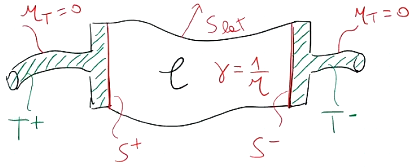
\includegraphics[width=0.5\linewidth]{modello_conduttore}
\end{figure}
Dato che il campo è necessariamente nullo in tutto il volume occupato
dai terminali, essi saranno equipotenziali.

La superficie esterna del conduttore invece, per rispettare il
principio di conservazione della carica rispetta la seguente
condizione in condizioni stazionarie
$$
\hat{n}\cdot\left(\vec{J}_2-\vec{J}_1\right) = 0
$$
Dove la regione 1 è quella del componente, la regione 2 è l'area
esterna, si può infatti porre $\vec{J}_2=0$ data la caratteristica
isolante dell'aria, ciò implica che \textbf{il vettore densità di corrente ha solo una componente tangenziale} alla superficie del conduttore
oppure che il conduttore è un tubo di flusso per il campo densità di 
corrente.

Fatta questa premessa si trova una condizione al contorno per il 
potenziale, ossia che la derivata normale sulla superficie laterale
per la funzione potenziale è nulla.
$$
\vec{J} = \gamma\vec{E} = -\gamma\nabla V \Rightarrow -\vec{J}_1\cdot
\hat{n} = \gamma \frac{\partial V_1}{\partial n} = 0
$$
Il potenziale sarà costante sulle superfici $S_1$ ed $S_2$ a causa
del potenziale sui morsetti, non varierà normalmente rispetto
alla superficie laterale, sono inoltre presenti anche due condizioni 
di Dirichlet, la soluzione esiste ed è unica.

\subparagraph{Circuito elementare con un generatore}
Si rappresentano due componenti collegati $C_1$ e $C_2$ e si 
rappresenta una linea $\Gamma$ chiusa orientata interna al circuito,
si applica la legge di Faraday-Neumann
\begin{figure}[H]
\centering
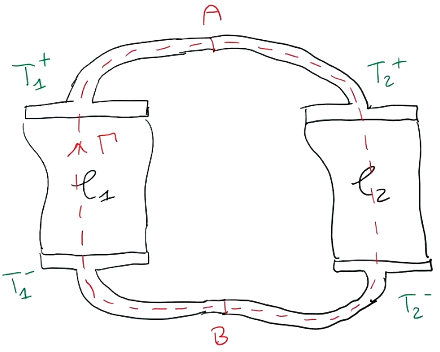
\includegraphics[width = 0.3\linewidth]{due_componenti_conduzione}
\end{figure}
$$
\oint_\Gamma\vec{E}\cdot\hat{t}dl = 0
$$
Nel caso generale ma se i materiali presenti in $C_1$ e $C_2$ sono
ohmici si avrà:
$$
\oint_\Gamma \eta\vec{J}\cdot\hat{t}dl = 0
$$
Il campo elettrico è quindi incapace di compiere lavoro affinché una 
carica di prova percorra quella linea chiusa, non ci può essere una 
corrente elettrica.

È necessario un campo ``elettromotore'' per stabilire la circolazione
di corrente, supposto per ipotesi nel conduttore $C_1$, ossia che
valga la relazione costitutiva
$$
\vec{J} = \gamma \left(\vec{E}+\vec{E}_m\right)
$$
dove $\vec{E}_m$ è il campo elettromotore di natura non puramente
elettrica (ad esempio elettro-chimica come una batteria).
Invertendo la precedente
$$
\vec{E} = \eta\vec{J} - \vec{E}_m
$$
Riscrivendo la legge di Faraday-Neumann
$$
\oint_{\Gamma}\vec{E}\cdot\hat{t}dl =  0 = \int_\Gamma \eta\vec{J}
\cdot\hat{t}dl - \int_\Gamma \vec{E}_m \cdot \hat{t}dl\Rightarrow
\int_\Gamma \vec{E}_m\cdot\hat{t}dl = \int_\Gamma \eta\vec{J}
\cdot\hat{t}dl
$$
L'integrale di linea del campo elettromotore viene indicato 
con
$\mathcal{E}$ e denominato ``forza elettromotrice'' lungo
la linea $\Gamma$, anche se dimensionalmente è un lavoro per unità
di carica e non una forza.

Se si assume il funzionamento a vuoto del circuito ossia $\vec{J} = 
0$, $C_1$ non collegato ad alcun componente 
\begin{figure}[H]
\centering
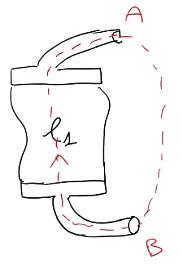
\includegraphics[width=0.3\linewidth]{generatore_a_vuoto}
\end{figure}
allora la F.E.M. è pari all'integrale 
$$
-\mathcal{E} = \oint_\Gamma \vec{E}\cdot\hat{t}dl \Rightarrow 
\mathcal{E} = \int_A^B \vec{E}\cdot\hat{t}dl = \left.v_{AB}\right|_{\Gamma_A}
$$
Dove $\Gamma_A$ è il tratto di circuitazione esterno al 
generatore.
La tensione a vuoto ai capi del generatore coincide proprio 
con la forza elettromotrice.

\subparagraph{Circuito elettrico}
Si vuole risolvere il problema di campo di corrente
stazionario nel seguente circuito
\begin{figure}[H]
\centering
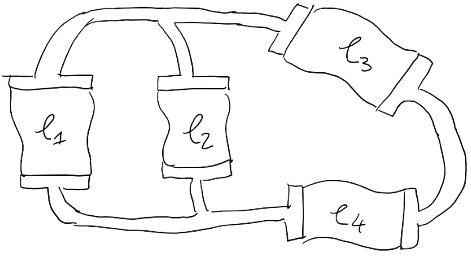
\includegraphics[width = 0.3\linewidth]{circuito_conduzione_stazionaria}
\end{figure}

Si considera il k-esimo componente $C_k$ collegato ai terminali $(r)$ ed $(s)$
detti anche nodi, essi saranno regioni equipotenziali.
\begin{figure}[H]
\centering
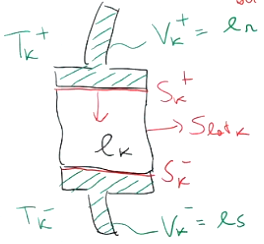
\includegraphics[width = 0.3\linewidth]{conduttore_singolo}
\end{figure}
Ricordando le equazioni della conduzione stazionaria
$$
\begin{aligned}
\nabla\cdot\vec{J} = 0 & \qquad \vec{J} = \gamma \vec{E} = -\gamma\nabla V\\
\vec{E} = -\nabla V & \qquad \nabla\cdot\left(-\gamma\nabla V\right) = 0 \Rightarrow \nabla^2 V = 0 \text{ nel materiale conduttore omogeneo}
\end{aligned}
$$
Nel conduttore il problema diventa
$$
\begin{cases}
\nabla^2 v &= 0  \text{ in } C\\
\left.V\right|_{S_k^+} &= e_r\\
\left.V\right|_{S_k^-} &= e_s\\
\left.\frac{\partial V}{\partial n}\right|_{S_{lat_k}} &= 0
\end{cases}
$$
Questo problema è ben posto e ammette soluzione unica, introduciamo una soluzione 
fondamentale 
$$
V^{(k)}: \begin{cases}
\nabla^2 V^{(k)} &= 0 \text{ in } C_k\\
V^(k) &= 1 \text{ su } S_k^+ \\
V^(k) &= 0 \text{ su } S_k^- \\
\frac{\partial V^{(k)}}{\partial n} &= 0 \text{ su } S_{lat_k}
\end{cases}
k = 1,...,l
$$
con $l$ il numero di bipoli. La soluzione del problema originario si ottiene con il
principio di sovrapposizione degli effetti:
$$
V = \sum_{k=1}^l a_kV^{(k)} \Rightarrow V(P) = (V_k^+ - V_k^-)V^{(k)}(P) + V_k^-
$$
Verifichiamo che questa sia proprio la soluzione ricordando che il Laplaciano 
di ogni singola funzione $V$ è nullo per ciascun bipolo
$$
\begin{aligned}
\nabla^2 V &= \nabla^2 V^{(k)} = 0\\
V|_{S_k^+} &= (V_k^+ - \cancel{V_K^-})\cdot 1 + \cancel{V_K^-} = V_k^+ \\
V|_{S_k^-} &= (V_k^+ - V_k^-)\cdot 0 + V_k^- = V_k^-
\end{aligned}
$$

Si considera ora una superficie $\Sigma$ composta dalla superficie $S_k^+$ e da una
superficie che taglia il terminale $(r)$ in aria, sia $S_r$ la parte di questa 
superficie che interseca il terminale, con normale entrante.
Se si applica il principio di conservazione della carica
$$
\oiint_\Sigma \vec{J}\cdot\hat{n} dS = 0 \Rightarrow i_{S_r} = i_{S_k^+} = \iint_{S_k} \vec{J}\cdot\hat{n}dS = \iint_{S_k^+}-\gamma\frac{\partial V}{\partial n} dS
$$
Sostituendo la soluzione di $V$ prima ottenuta
$$
i_{S_r} = i_k = \iint_{S_k^+} -\gamma\left(V_k^+ - V_k^-\right)\frac{\partial V}{\partial n}^{(k)} dS = \left( \iint_{S_k^+} -\gamma\frac{\partial V}{\partial n}^{(k)} dS \right)
v_k = G_k v_k
$$
dove $v_k$ è proprio la tensione ai capi del componente mentre il coefficiente $G_k$
tra parentesi è il rapporto tra una corrente e una tensione ossia una conduttanza.
Definendo $R_k = \frac{1}{G_k}$ si ottiene la legge di Ohm in forma integrale
ossia
$$
v_k = R_ki_k
$$

S si suppone che nel componente sia presente un campo elettromotore, con il PSE
si sommano le due tensioni
$$
\begin{cases}
v_k' = \mathcal{E} & \text{a vuoto}\\
v_k'' = R_ki_k 
\end{cases}\Rightarrow
v_k = v_k' + v_k'' = \mathcal{E} + R_ki_k
$$
Ossia l'equazione caratteristica di un generatore reale di tensione formato da uno ideale
con una resistenza in serie.

\subsection{Interconnessione di componenti a due terminali}
\begin{figure}[H]
\centering
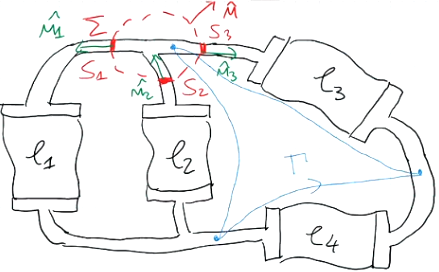
\includegraphics[width = 0.4\linewidth]{circuito_conduzione_stazionaria_nodo}
\end{figure}
\paragraph{LKC}
Si consideri una qualsiasi superficie chiusa $\Sigma$ che tagli tutti e soli i terminali
afferenti ad un nodo, tutte le superfici di questo tipo godono della proprietà di
equivalenza, si può costruire una classe di equivalenza ed applicare i risultati ottenuti
dallo studio della singola superficie a tutte le altre ad essa equivalenti.
Presa una superficie d'esempio si applica il principio di conservazione delle cariche:
$$
\oiint_\Sigma \vec{J}\cdot\hat{n}dS = 0\ \forall\ \Sigma \text{ di quella classe}
$$
Sfruttando la proprietà di additività dell'integrale
$$
\iint_{S_1}\vec{J}\cdot\hat{n}dS + \iint_{S_2}\vec{J}\cdot\hat{n}dS + \iint_{S_3}\vec{J}\cdot\hat{n}dS + \cancel{\iint_{S_{\text{aria}}} \vec{J}\cdot\hat{n}dS} =0
$$
Si può scegliere l'orientamento delle superfici $S_1,S_2,S_3$ in modo 
arbitrario come evidenziato dalle frecce in verde in figura.
Con questa configurazione vanno riscritti gli integrali
$$
\hat{n}_1 = \hat{n},\ \hat{n}_2 = -\hat{n},\ \hat{n}_3 = \hat{n}
$$
$$
\iint_{S_1}\vec{J}\cdot\hat{n}_1dS - \iint_{S_2}\vec{J}\cdot\hat{n}_2dS + \iint_{S_3}\vec{J}\cdot\hat{n}_3dS =0 \Leftrightarrow i_1 - i_2 + i_3 = 0
$$
Si ricava da questa relazione la legge di Kirchhoff per le correnti
$$
\forall\ \text{nodo }\sum_{k} (\pm) i_k = 0
$$
Valida in conduzione stazionaria o in caso di valori ``lentamente'' variabili
ossia in cui si possono trascurare i fenomeni propagativi del campo elettrico.

\paragraph{LKT}
Si considerino linee $\Gamma$ (in azzurro) ragionevoli che toccano i terminali dei 
componenti che costituiscono una maglia. Si può applicare ad una di queste linee la legge di 
Faraday-Neumann
$$
\oint_{\Gamma} \vec{E}\cdot\hat{t}dl = 0\ \forall\Gamma \text{ di quella classe}
$$
Suddividendo la linea $\Gamma$ si possono dividere gli integrali rispettando il verso
arbitrario di definizione delle tensioni sui singoli componenti ottenendo dunque
$$
v_2-v_4-v_3 = 0
$$
$$
\forall\ \text{ maglia } \sum_h (\pm) v_h = 0
$$
Anche in questo caso il limite del modello è la velocità di propagazione del campo.

\subsection{Resistori filiformi}
\begin{figure}[H]
\centering
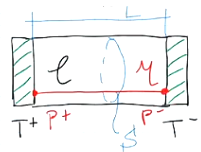
\includegraphics[width=0.4\linewidth]{conduttore_cilindrico}
\end{figure}
Si consideri un cilindro di materiale con due elettrodi, una sezione $S$ e una lunghezza 
$L$, una resistività $\eta$ assegnata e costante in $C$.
Si calcola la tensione $v$ tra i terminali considerando una linea retta tra essi
$$
v = \int_{p^+}^{p^-} \vec{E}\cdot\hat{t}dl = \int_{p^+}^{p^-} \eta\vec{J}\cdot\hat{t}dl
$$
Ricordando però che $\sqrt{S} << L \Rightarrow \vec{J} = \frac{i}{S}\hat{t}$ sostituendo
$$
v = \int_{p^+}^{p^-} \eta\frac{i}{S}dl \stackrel{(1)}{=} \eta\frac{i}{S} L = \eta\frac{L}{S}i = R\cdot i
$$
Il passaggio $(1)$ è valido se la sezione del cilindro è costante, con $R=\eta\frac{L}{S}$ 
detta anche seconda legge di Ohm.

\newpage
\subsection{Valutazione della resistenza di terra}
Si considerino due elettrodi sferici concentrici di raggio $a$ e $b$, ai quali colleghiamo 
un generatore che sostiene la tensione $v$ come in figura
\begin{figure}[H]
\centering
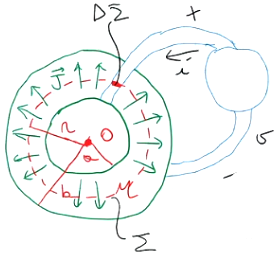
\includegraphics[width = 0.4\linewidth]{resistenza_terra}
\end{figure}
Si può determinare la corrente $i$ uscente dal generatore se supponiamo che tra i due mezzi
esista un elemento di resistività $\eta$, ci sarà un campo elettrico e di densità di 
corrente radiale dovuto alla 
distribuzione di carica positiva sull'elettrodo interno e negativa su quello esterno.
Utilizzando il metodo volt-amperometrico si ricava la resistenza del materiale
$$
R = \frac{v}{i}
$$
Si considera una superficie sferica di centro $O$ e raggio $r$ si applica ancora una volta
il principio di conservazione della carica alla superficie $\Sigma$ ottenuta
$$
\oiint_\Sigma \vec{J}\cdot\hat{n}dS = 0
$$
Per ragioni di simmetria sferica la densità di corrente ha la sola componente radiale
$\vec{J} = J_r(r)$ è quindi un problema monodimensionale.
$$
\iint_{\Sigma -\Delta\Sigma} \vec{J}\cdot\hat{n}dS + \iint_{\Delta\Sigma} \vec{J}
\cdot\hat{n}dS = 0
$$
il contributo che attraversa la superficie $\Delta\Sigma$ è $-i$ mentre l'area
dell'altra superficie si può approssimare alla superficie sferica di raggio $r$ con area
pari a $4\pi r^2$.
$$
4\pi r^2 J_r(r) - i = 0 \Rightarrow J_r(r) = \frac{i}{4\pi r^2}
$$
Il campo sarà dunque
$$
\vec{E} = \eta\vec{J} = \frac{\eta}{4\pi r^2} i
$$
\newpage
La tensione tra due punti posti sugli elettrodi sarà
$$
v = V(P_1) - V(P_2) = \int_{P_1}^{P_2} \vec{E}\cdot\hat{t}dl = \int_{r_1}^{r_2}
\eta\frac{i}{4\pi r^2} dr = \eta \frac{i}{4\pi} \left[-\frac{1}{r}\right]_a^b  = 
$$
$$
= \frac{\eta}{4\pi}\left(\frac{1}{a} -\frac{1}{b}\right) i \Rightarrow R = \frac{v}{i} = 
\frac{\eta}{4\pi}\left(\frac{1}{a} - \frac{1}{b}\right)
$$
La resistenza di terra si ottiene facendo tendere il raggio del dispersore esterno $(b)$
all'infinito come se fosse un piano, la formula per calcolare la resistenza di terra
dipende solo dal raggio del dispersore $a$ e dalla resistività del suolo
$$
R_T = \frac{\eta}{4\pi}\frac{1}{a}
$$

\subparagraph{Dispersore emisferico}
Si collega un dispersore emisferico interrato nel piano di terra, si collega un
generatore di tensione ad un punto del dispersore e un punto abbastanza
distante nel piano di terra.
\begin{figure}[H]
\centering
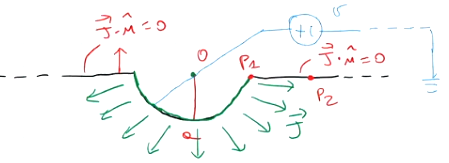
\includegraphics[width = 0.4\linewidth]{dispersore_emisferico}
\end{figure}
Analizzando le condizioni al contorno del suolo
$$
\vec{J}\cdot\hat{n} = 0
$$
la densità di corrente sarà dunque ancora radiale rispetto al dispersore,
mantenendo il vantaggio matematico della simmetria $(\vec{J} = J_r(r))$
la superficie sarà però la metà della sfera e di conseguenza 
$$
J_r(r) = \frac{i}{2\pi r^2}
$$
Presa dunque una linea che congiunge un punto tangente al dispersore e un punto a
sufficiente distanza si può calcolare la tensione
$$
V(P_1) - V(P_2) = \int_{P_1}^{P_2} \vec{E}\cdot\hat{t} dl = -\int_{r_1}^{r_2} \eta\frac{i}{2\pi r^2} dr = \frac{\eta}{2\pi} \left[-\frac{1}{r}\right]_a^{r_2}\cdot i
$$
$$
V(P_1)-V(P_2) = \frac{\eta}{2\pi}\left(\frac{1}{a}-\frac{1}{r_2}\right) i
$$
La normativa specifica il limite massimo della \textit{tensione di passo}
ossia la tensione presente a distanza di un metro (un passo) $V(r) - V(r+1)$
$$
\frac{\eta}{2\pi}\left(\frac{1}{r} - \frac{1}{r+1}\right) i = \frac{\eta}{2\pi}\left(\frac{r+1 - r}{r^2 + r}\right) i = \frac{\eta}{2\pi}\left(\frac{1}{r^2+r}\right) i
$$
L'andamento della tensione di passo è del tipo $\frac{1}{r^2}$, per questo motivo è 
necessario prevedere una zona di sicurezza nell'intorno del dispersore non calpestabile.

\subsection{Bilancio energetico in un circuito elementare}
Preso un circuito con due componenti collegati, un generatore ed un utilizzatore $C_1$ e 
$C_2$ collegati mediante gli elettrodi $T^+$ e $T^-$, si orientano le regioni dei 
terminali. 
\begin{figure}[H]
\centering
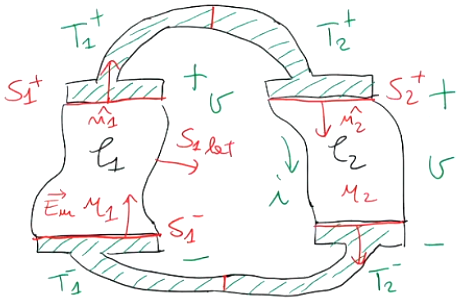
\includegraphics[width=0.6\linewidth]{generatore_utilizzatore}
\end{figure}
Si considerano le regioni dei terminali conduttori ideali
$$
\begin{aligned}
T_1^+ \cup T_2^+ &\qquad \vec{E} = 0,\ \vec{J} \neq 0\\
T_1^- \cup T_2^- &\qquad \vec{E} = 0,\ \vec{J} \neq 0
\end{aligned}
$$
mentre le regioni dei conduttori saranno caratterizzate dalle seguenti espressioni
$$
\begin{aligned}
\vec{J} &= \gamma_1 (\vec{E}+\vec{E_m}) \qquad &\text{in } C_1\\
\vec{J} &= \gamma_2\vec{E} \qquad &\text{in } C_2
\end{aligned}
$$
La potenza necessaria a muovere le cariche nel circuito è misurabile con l'integrale del lavoro per unità di tempo e per unità di carica nel volume
$$
P^{(a)}_{C_1} = \iiint_{C_1} \vec{E}\cdot\vec{J} dV = \iiint_{C_1} \left(\eta_1\vec{J} - 
\vec{E}_m\right)\cdot\vec{J} dV = \iiint_{C_1} \eta_1 |\vec{J}|^2dV - \iiint_{C_1} \vec{E}_m\cdot\vec{J}dV
$$
Il primo termine sicuramente maggiore di zero è la dissipazione per effetto Joule
della resistenza interna del generatore. Il secondo termine (negativo) è l'energia 
assorbita dal generatore, il segno opposto indica che è erogata.

Ricordando che $nabla\cdot(f\vec{v}) = f\nabla \cdot\vec{v} + \nabla f \cdot\vec{v}$ e che
nelle ipotesi di conduzione stazionaria $\vec{E} = -\nabla V $ e $\nabla\cdot\vec{J}= 0$

allora
$$
\nabla\cdot(V\vec{J}) = \cancel{V\nabla\cdot\vec{J}} + \nabla V \cdot \vec{J} = -\vec{E}\cdot\vec{J}
$$
sostituendo nell'integrale
$$
\iiint_{C_1} - \nabla\cdot(V\vec{J}) dV \stackrel{\text{T. divergenza}}{=} \iint_{\partial C_1} - V\vec{J}\cdot\hat{n}dS = \iint_{S_1^+}-V_1^+\vec{J}\cdot\hat{n}_1dS - \iint_{S_1^-}-V_1^-\vec{J}\cdot\hat{n}_1dS
$$
$$
-V_1^+ i + V_1^-i = -(V_1^+-V_1^-)\cdot i = - v\cdot i = \iiint_{C_1} \eta_1 |\vec{J}|^2dV - \iiint_{C_1} \vec{E}_m\cdot\vec{J}dV
$$
che è proprio la potenza assorbita dal generatore.

Si calcola ora la potenza assorbita dal carico $(C_2)$
$$
P_{C_2}^{(a)} = \iiint_{C_2} \vec{E}\cdot\vec{J} dV = \iiint_{C_2} \eta_2 |\vec{J}|^2 dV = v\cdot i
$$
utilizzando la stessa identità vettoriale, in conclusione
$$
P_{C_1}^{(e)} = -P_{C_1}^{(a)} =  \iiint_{C_1} \vec{E}_m\cdot\vec{J}dV - \iiint_{C_1} \eta_1 |\vec{J}|^2dV = v\cdot i = \iiint_{C_2} \eta_2 |\vec{J}|^2 dV = P_{C_2}^{(a)}
$$
ossia si è dimostrato mediante la formulazione campistica che la potenza erogata
dal generatore è pari a quella assorbita dal resistore.
Il modello circuitale equivalente è pari a quello del generatore reale con resistenza
interna $R_i$ collegato al carico $R$.
$$
P_{gen}^{(e)} = v\cdot i = (E_0 -R_i i ) = E_0 i - R_i i^2 = P_R^{(a)} = Ri^2
$$

\subsection{Analisi FEM conduzione stazionaria}
Si misura la resistenza di un fluido attraversato da corrente.
\begin{figure}[H]
\centering
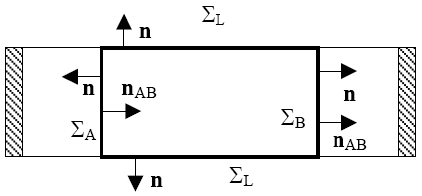
\includegraphics[width=0.4\linewidth]{conduzione_FEM}
\end{figure}
Si ricordano le ipotesi di solenoidalità di $\vec{J}$ e conservatività di $\vec{E}$
\begin{align*}
\oint_\gamma \vec{E}\cdot\hat{t} dl = 0 &\qquad \forall\ \gamma \\
\oiint_\Sigma \vec{J}\cdot\hat{n} dS = 0 &\qquad \forall\ \Sigma
\end{align*}
Si consideri una linea che unisca i due elettrodi, la scelta non è importante
essendo il campo $\vec{E}$ conservativo.
La componente normale alla superficie laterale è nulla a causa dell'isolamento
dell'aria mentre i flussi attraverso le superfici $\Sigma_A$ e $\Sigma_B$ sono 
uguali e opposti, o identici a seconda di come si considerano le normali alle 
superfici, in conclusione si può dire che la corrente che attraversa la superficie $A$
è identica a quella che attraversa la superficie $B$.

Il modello differenziale in analisi è il seguente
\begin{align*}
&\nabla\times\vec{E} = 0 \Rightarrow \vec{E} = -\nabla U\\
&\nabla\cdot\vec{J} = 0 \Rightarrow \nabla^2 U = 0 \quad \text{con }\vec{J} = \sigma\vec{E}\\
&U|_{l_1}  = V_1\\
&U|_{l_2} = 0 \\
&\left.\frac{\partial U}{\partial \hat{n}}\right|_{l_3 \cup l_4} =0
\end{align*}

Si esegue lo strumento \textit{pdetool} e si definisce una geometria rettangolare,
si impostano le condizioni di Dirichlet alle superfici degli elettrodi e Neumann a quelle 
laterali.
In PDE Mode si imposta l'equazione ellittica con costanti unitarie, si imposta il meshing
è si calcola la soluzione.
Per calcolare la resistenza si può esportare la mesh e calcolare l'intensità di corrente su 
una faccia.
Per calcolare l'intensità di corrente occorre dunque integrare il flusso della densità
di corrente per la superficie di frontiera.
La superficie è discretizzata, vanno quindi considerati i singoli triangoli
che compongono la superficie laterale, si approssima la derivata al rapporto incrementale,
preso un punto sull'ascissa $x=0$ e ordinata $y$, si sa con certezza che ha potenziale 
unitario perché imposto dal problema, resta quindi da stimare il potenziale nel 
punto $(x+\Delta x,y)$ per calcolarne la derivata
$$
\frac{V(x+\Delta x,y) - V (0,y)}{\Delta x}\simeq \frac{\partial V}{\partial x} (0,y) +o(\Delta x^2)
$$
Sfruttando il comando ``tri2grid'' è possibile interpolare una mesh triangolare
in una griglia rettangolare riportando i valori corretti
\begin{lstlisting}[style=Matlab-editor,language = Matlab]
%plot mesh
figure();
pdemesh(p,e,t);
%definizione ascissa di controllo
dx = 0.1;
x = dx*ones(20,1)-0.5;
y = linspace(0,0.5,20);
%Plot della linea di controllo sulla mesh, colore magenta
hold on;
plot(x,y,'m');
%Interpolazione della mesh
u_dx = tri2grid(p,t,u,x,y);
%Calcolo rapporto incrementale rispetto al potenziale 1 di partenza
du_dx = (u_dx-1)/dx;
Ex = -du_dx;
%Media del campo
mean(Ex)
%Conducibilita' e densita' di corrente
gamma = 1;
Jx = gamma*Ex
%Dimensioni conduttore
h = 0.5;
Lz = 1;
S = h * Lz;
%Stima della corrente
i = mean(mean(Jx))*S
\end{lstlisting}
È possibile ripetere l'analisi per un conduttore emisferico interrato e confrontarla
con la resistenza analitica.

Work in progress...
\subparagraph{Si ringraziano infinitamente le persone che hanno contribuito}
\begin{itemize}
\item Tommaso Pio Pergamo
\end{itemize}
\end{document}
